%\documentclass{article}
\documentclass{report}
%\usepackage[utf8]{vietnam}
\usepackage[utf8]{inputenc}
\usepackage{anyfontsize,fontsize}
\changefontsize[13pt]{13pt}	
\usepackage{commath}
\usepackage{parskip,setspace}
\usepackage{xcolor}
\usepackage{amssymb}
\usepackage[d]{esvect}
\usepackage[nottoc,notlot,notlof]{tocbibind}
\usepackage{slashed,cancel}
\usepackage{indentfirst,titlesec}
\usepackage{pdfpages}
\usepackage{graphicx,subcaption,floatrow,adjustbox,rotating}
\usepackage{nccmath}
\usepackage{mathtools}
\usepackage{amsfonts,esint}
\usepackage[printonlyused,withpage]{acronym}
\usepackage{wrapfig}
\usepackage[toc,page]{appendix}
\usepackage{amsmath,systeme}
\usepackage[thinc]{esdiff}
\usepackage{hyperref,tikz}
\usepackage{bm,physics,nicematrix}
\usepackage[numbers,comma,sort&compress]{natbib}
%footnote
\usepackage{fancyhdr}
\usepackage{array,tocbibind}
\usepackage{enumitem}
\pagestyle{empty}


\usepackage{geometry}
\geometry{
	a4paper,
	total={170mm,257mm},
	left=20mm,
	top=20mm,
}



\newcommand{\image}[1]{
	\begin{center}
		\includegraphics[width=0.5\textwidth]{pic/#1}
	\end{center}
}




\renewcommand{\l}{\ell}
\newcommand{\dps}{\displaystyle}

\newcommand{\f}[2]{\dfrac{#1}{#2}}
\newcommand{\at}[2]{\bigg\rvert_{#1}^{#2} }


\renewcommand{\baselinestretch}{1.5}



\hypersetup{
	colorlinks=true,
	linkcolor=black,
	filecolor=magenta,      
	urlcolor=cyan,
	pdftitle={UT},
	citecolor=green,
	pdfpagemode=FullScreen,
}

\urlstyle{same}

\titleformat{\chapter}[display]
{\centering\large\bfseries} 
{\textbf{\MakeUppercase{\chaptername}} \ \thechapter\vspace{15pt}}{20pt}
{\large} 

%\newcommand{\thesistitlee}{Three-band tight binding model for TMD monolayers in the presence of a magnetic field}
\newcommand{\thesistitlee}{Hofstadter butterfly in transistion metal dichalcogenide monolayers}
\newcommand{\address}{NATIONAL UNIVERSITY OF HO CHI MINH CITY UNIVERSITY OF SCIENCE}
\newcommand{\department}{FACULTY OF PHYSICS - ENGINEERING PHYSICS}
\newcommand{\thesisauthor}{Tran Khoi Nguyen}
\newcommand{\thesisadvisor}{Your Advisor's Name}
\newcommand{\graddate}{Ho Chi Minh City, 2025}
\newcommand{\thesisdedication}{To all the Ph.D. pursuing brave souls}

\newlist{abbrv}{itemize}{1}
\setlist[abbrv,1]{label=,labelwidth=1in,align=parleft,itemsep=0.1\baselineskip,leftmargin=!}
\begin{document}
\setlength{\parindent}{20pt}
\begin{titlepage}
	\begin{center}
		{\bfseries

		{\large {\bf \address}}\\
		{{\textbf{\department}}}\\
		{---------------------o0o--------------------}
		\vspace{1.5cm}
	
		{\large {\bf UNDERGRADUATE THESIS}}\\
		\vspace{3.0cm}

		}

	\end{center}
	\textit{\textbf{\underline{Thesis title:}}}\\
	\begin{center}
		{\bfseries

			{\largerrr\thesistitlee}
			\vspace{1in}

		}
	\end{center}
	\noindent
	\makebox[\textwidth]{\hfill\makebox[3in]{\hrulefill}}\\
	\begin{center}
		\makebox[\textwidth]{\hfill\makebox[3in]{\hfill \textbf{Student: Tran Khoi Nguyen}\hfill}}
		\makebox[\textwidth]{\hfill\makebox[3in]{\hfill \textbf{Supervisor: Dr. Huynh Thanh Duc}\hfill}}
	\end{center}
	\begin{tikzpicture}[remember picture, overlay]
		\draw[line width=2pt]
		([xshift=1.5cm, yshift=1.5cm] current page.south west)
		rectangle
		([xshift=-1.5cm, yshift=-1.5cm] current page.north east);
	\end{tikzpicture}
	\begin{center}
		\vspace{2.5in}
		{\graddate}
	\end{center}
\end{titlepage}
\begin{titlepage}
	\begin{center}
		{\bfseries

		{\large {\bf \address}}\\
		{{\textbf{\department}}}\\
		\vspace{2.5cm}

		{\large {\bf UNDERGRADUATE THESIS}}\\
		\vspace{3.0cm}

		}

	\end{center}
	\textit{\textbf{\underline{Thesis title:}}}\\
	\begin{center}
		{\bfseries

			{\largerrr\thesistitlee}
			\vspace{1in}

		}
	\end{center}
	\noindent
	\makebox[\textwidth]{\hfill\makebox[3in]{\hrulefill}}\\
	\begin{center}
		\makebox[\textwidth]{\hfill\makebox[3in]{\hfill \textbf{Student: Tran Khoi Nguyen}\hfill}}
		\makebox[\textwidth]{\hfill\makebox[3in]{\hfill \textbf{Supervisor: Dr. Huynh Thanh Duc}\hfill}}
	\end{center}
	\begin{center}
		\vspace{2.5in}
		{\graddate}
	\end{center}
\end{titlepage}

\newpage
\pagenumbering{roman}
\pagestyle{fancy}
\renewcommand{\headrulewidth}{0pt}
\fancyhf{}
\fancyfoot[C]{\hspace{0cm} \thepage}
\setcounter{page}{1}
\begin{center}
	{\bfseries
		
		{\large {\bf \address}}\\
		{{\textbf{\department}}}\\
		\vspace{2.5cm}
		
		{\large{\bf \thesistitlee}}\\
		\vspace{3.0cm}
		
	}
	
\end{center}
\textbf{ABSTRACT}

Hofstadter's butterfly has been studied experimentally for 50 years. It was first discovered by computer scientist Douglas Hofstadter. This thesis explores the electronic phenomena in material systems, particularly focusing on monolayer \ac{TMD}. A key focus is on understanding Hofstadter physics. We begin by studying a minimal three-band \ac{TBM} in order to describe the electronic structure of \ac{TMD} monolayer. We, then, analyze the resulting Hofstadter spectrum under an external magnetic field, reavling the rich fractal stucture. Building on this framework, we further explore related quantum phenomena including Landau levels and quantum Hall effect.

\chapter*{GUARANTEE}


\chapter*{ACKNOWLEDGMENTS}
This thesis would not have been possible without the help and support of a large number of individuals. Firstly, I would like to thank my family members, especially my beloved mother and my sister, who have totally encouraged me on my path of becoming a scientist and helped me trenmendously in all ways possible. Without them, I would not have enough much confidence to finish this. Thank you.

I am deeply greeted to my supervisor Dr. Huynh Thanh Duc from the Institute of Physics, Ho Chi Minh city, who taught me not only knowledges, gave me advise but also wholeheartedly encouraged and guided me every steps of the way. I would like to thank Master Le Minh Chau from the Institute of Physics, who helped me at the very first step of this thesis. I would also like to acknowledge with gratitude to Dr. Vu Quang Tuyen, Dr. Vo Quoc Phong and Dr. Nguyen Huu Nha from the Department of Theoretical Physics. They have trully inspired me on the way becoming a physicist. 

Finally, I would like to thank my colleagues at the University of Science including Dao Duy Tung, Le Quoc Duy, Ho Ngo Thanh Khoa, Pham Hoang Minh Quang, Truong Anh Duy, Pham Nguyen Thanh Dat.
\renewcommand{\contentsname}{TABLE OF CONTENTS}
\tableofcontents
\renewcommand{\listfigurename}{LIST OF FIGURES}
\listoffigures
\newpage
\renewcommand{\listtablename}{LIST OF TABLES}
\listoftables
\newpage
\chapter*{\MakeUppercase{List of Abbreviations}}
%\addcontentsline{toc}{chapter}{LIST OF ABBREVIATIONS}
\chaptermark{List of Abbreviations}
\begin{acronym} % Give the longest label here so that the list is nicely aligned
	\acro{TMD}{transition metal dichacolgenides}
	\acro{TB}{tight-binding}
	\acro{TBM}{tight-binding model}
	\acro{NN}{nearest-neighbor}
	\acro{2D}{two-dimensional}
	\acro{BZ}{Brillouin zone}
	\acro{GGA}{generalized-gradient approximation}
	\acro{SOC}{spin orbit coupling}
	\acro{LLs}{Landau levels}
	\acro{QHE}{Quantum Hall effect}
	\acro{IQHE}{integer Quantum Hall effect}
	\acro{FQHE}{fractional Quantum Hall effect}
	\acro{EFA}{Envelope Function Approximation}
	\acro{BCH}{Baker-Campbell-Hausdorff}
	\acro{TKNN}{Thouless-Kohmoto-Nightingale-Nijs}
	\acro{SBE}{semiconductor Bloch equations}
	\acro{LCAO}{linear combination of atomic orbitals}
	\acro{TNN}{three-band third-nearest-neighbor-model}
	\acro{LDA}{local-density approximation}
	\acro{VG}{velocity gauge}
	\acro{HHG}{high harmonic generation}
	\acro{HSG}{high-order sideband generation}
\end{acronym}
\newpage
\chapter*{Abstract}
\textbf{Keywords}:
\newpage
\pagenumbering{arabic}
\chapter{\textbf{INTRODUCTION}}

The idea behind Hofstadter’s butterfly is that you’re looking at how the band structure of electrons moves when you have the magnetic field on one axis and the electrons’ energies on the other, and plotted on that diagram, the band forms a fractal structure that looks like a butterfly

\chapter{\textbf{THEORY}}
\section{Three-band tight binding method without magnetic field}\label{Section 2}
\begin{figure}[H]
	\centering
	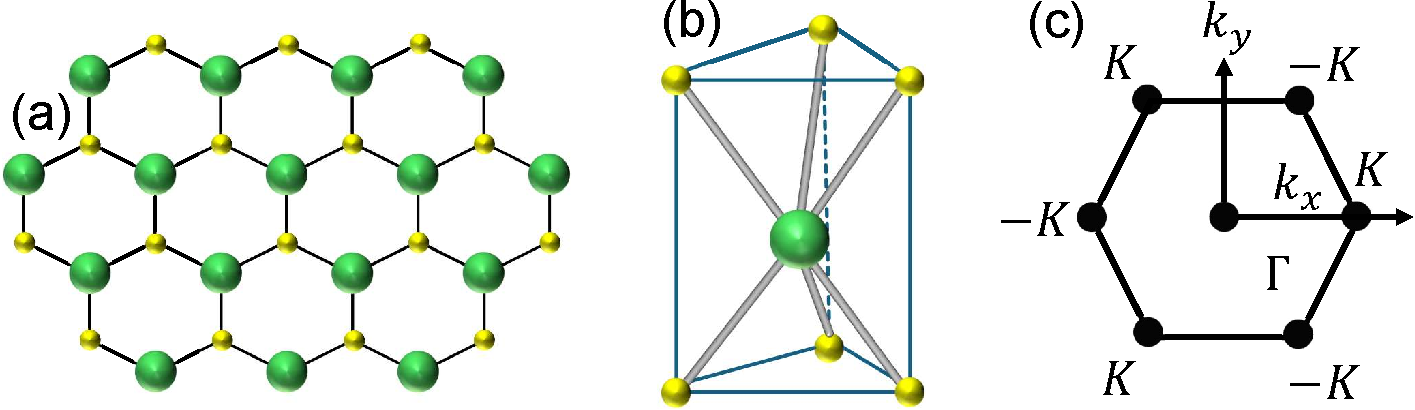
\includegraphics[width=\linewidth]{pic/lattice_crop.pdf}
	\caption[TMD structure and its first Brillouin zone.]{\label{fig:Lattice} Top view of monolayer $MX_{2}$. The large sphere is $M$ atom and the small sphere is $X$.}
\end{figure}
The time-indepentdent Schr\"{o}dinger equation for an eletron in the crystal has the form
\begin{gather}
	\left[-\f{\hbar^{2} \nabla^{2}}{2m} + U_{0}(\mathbf{r})\right] \psi_{\lambda,\mathbf{k}}(\mathbf{r}) = \varepsilon_{\lambda}(\mathbf{k}) \psi_{\lambda,\mathbf{k}}(\mathbf{r}),
\end{gather}
where $U_{0}(\mathbf{r})$ is the periodic lattice potential, $\psi_{\lambda,\mathbf{k}}(\mathbf{r})$ is the Bloch wavefunction of an electron in band $\lambda$ with wave vector $\mathbf{k}$ and $\varepsilon_{\lambda}(\mathbf{k})$ is the band structure.

In the \acf{TBM}, the single-electron Bloch wavefunction can be expressed in terms of atomic orbitals as follows
\begin{gather}
	\psi_{\lambda,\mathbf{k}}(\mathbf{r}) = \sum_{j,i} C_{ji}^{\lambda}(\mathbf{k}) \sum_{\mathbf{R}} e^{i\mathbf{k}\cdot(\mathbf{R+\mathbf{r}_{i}})} \phi_{j}(\mathbf{r} - \mathbf{R} - \mathbf{r}_{i}),
\end{gather}
where $\phi_{j}(\mathbf{r} - \mathbf{R} - \mathbf{r}_{i})$ is the orbital $j$ of an atom $i$ localized on a lattice site $\mathbf{R}$, in which $\mathbf{r}_{i}$ is the relavetive position of the atom $i$ in the unit cell, and $C_{ji}^{\lambda}(\mathbf{k})$ are the coefficents of linear expansion.

The unit cell of \ac{TMD} involve one transition metal atom $M$ and two chalcogenide atoms $X$. From the \textit{ab initio} calculations, it is shown that the electron states near the band edges of $MX_{2}$ are mainly contributed from the three $d$ orbital of $M$ atom, namely $d_{z^{2}},d_{xy},d_{x^{2}-y^{2}}$ \cite{PhysRevB.88.085433}. Since only the orbitals of atom $M$ is included, we ignore the sum over the atom $\mathbf{r}_{i}$ in the unit cell in Eq. (2.2). This model is called the three-band tight binding model. The three orbitals's wave function of $M$ atom are denoted as
\begin{gather}
	\ket{\phi_{1}} = \ket{d_{z^{2}}} ; \quad \ket{\phi_{2}} = \ket{d_{xy}} ; \quad \ket{\phi_{3}} = \ket{d_{x^{2} - y^{2}}}.
\end{gather}
The Bloch wavefunction in this model has the form
\begin{gather}
	\psi_{\lambda,\mathbf{k}}(\mathbf{r}) = \sum_{j=1}^{3} C_{j}^{\lambda}(\mathbf{k}) \sum_{\mathbf{R}} e^{i \mathbf{k \cdot R}} \phi_{j}(\mathbf{r} - \mathbf{R}).
\end{gather}
The coefficents $C_{j}^{\lambda}(\mathbf{k})$ are the solutions of the eigenvalue equation
\begin{gather}
	\sum_{jj'}^{3} \left[H_{jj'}^{\text{TB}}(\mathbf{k}) - \varepsilon_{\lambda}(\mathbf{k}) S_{jj'}(\mathbf{k})\right] C_{j}^{\lambda}(\mathbf{k}) = 0,
\end{gather}
where
\begin{gather}
	H_{jj'}^{\text{TB}}(\mathbf{k}) = \sum_{\mathbf{R}} e^{i \mathbf{k \cdot R}} \bra{\phi_{j}(\mathbf{r})} \left[-\f{\hbar^{2} \nabla^{2}}{2m} + U_{0}(\mathbf{r})\right] \ket{\phi_{j'}(\mathbf{r - R})},
\end{gather}
and
\begin{gather}
	S_{jj'}(\mathbf{k}) = \sum_{\mathbf{R}} \bra{\phi_{j}(\mathbf{r})} \ket{\phi_{j'}(\mathbf{r - R})} \approx \delta_{jj'}.
\end{gather}

The three-band tight-binding model often called the \ac{NN} since it only includes nearest-neighbor hopping does a decent job matching \textit{ab initio} results near the band edges. However, it starts to break down in other parts of the band structure. This is because the model completely ignores the $p$ orbitals from the $X$ atoms, which stil contributions to the conduction bands at $\Gamma$ and the valence bands at $M$. The matrix elements of the \ac{TB} Hamiltonian Eq. (2.6) are
\begin{equation}
	\begin{aligned}
		H_{jj'}^{\text{NN}}(\mathbf{k})
		 & = \mathcal{E}_{jj'}(\mathbf{0}) + e^{i\mathbf{k}\cdot \mathbf{R}_{1}}\mathcal{E}_{jj'}(\mathbf{R}_{1}) + e^{i\mathbf{k}\cdot \mathbf{R}_{2}}\mathcal{E}_{jj'}(\mathbf{R}_{2}) + e^{i\mathbf{k}\cdot \mathbf{R}_{3}}\mathcal{E}_{jj'}(\mathbf{R}_{3}) \\
		 & + e^{i\mathbf{k}\cdot \mathbf{R}_{4}}\mathcal{E}_{jj'}(\mathbf{R}_{4}) + e^{i\mathbf{k}\cdot \mathbf{R}_{5}}\mathcal{E}_{jj'}(\mathbf{R}_{5}) + e^{i\mathbf{k}\cdot \mathbf{R}_{6}}\mathcal{E}_{jj'}(\mathbf{R}_{6}),
	\end{aligned}
\end{equation}
where
\begin{gather}
	\mathcal{E}_{jj'}(\mathbf{R}) = \bra{\phi_{j}(\mathbf{r})} \left[-\frac{\hbar \nabla^{2}}{2m} + U_{0} (\mathbf{r})\right] \ket{\phi_{j'}(\mathbf{r-R})},
\end{gather}
and
\begin{equation}
	\begin{aligned}
		\mathbf{R}_{1} & = (a,0), \quad \mathbf{R}_{2} = \left(\f{a}{2}, - \f{a\sqrt{3}}{2}\right), \quad \mathbf{R}_{3} = \left(-\f{a}{2},-\f{a\sqrt{3}}{2}\right), \\
		\mathbf{R}_{4} & = (-a,0), \quad \mathbf{R}_{5} = \left(-\f{a}{2}, \f{a\sqrt{3}}{2}\right), \quad \mathbf{R}_{3} = \left(\f{a}{2},\f{a\sqrt{3}}{2}\right).
	\end{aligned}
\end{equation}
Here, $\mathbf{R}_{1-6}$ are the positions of the nearest neighbors $M$ atoms, see Fig.
%%%%% Table
\begin{table}[h]
	\begin{equation*}
		\renewcommand{\arraystretch}{1.5}
		\begin{NiceArray}{c c c c c c c}
			\hline
			\hline
			g_{n}                  & x'                                   & y'                                  & z' & z'^{2} & x'y'                                               & \frac{1}{2}(x'^{2} - y'^{2})                        \\
			\hline
			E                      & x                                    & y                                   & z  & z^{2}  & xy                                                 & \frac{1}{2}(x^{2} - y^{2})                          \\
			C_{3}(\frac{-2\pi}{3}) & -\frac{1}{2}x + \frac{\sqrt{3}}{2} y & -\frac{\sqrt{3}}{2}x - \frac{1}{2}y & z  & z^{2}  & -\frac{1}{2}xy + \frac{\sqrt{3}}{4}(x^{2} + y^{2}) & -\frac{\sqrt{3}}{2} xy - \frac{1}{4}(x^{2} - y^{2}) \\
			C_{3}(\frac{-4\pi}{3}) & -\frac{1}{2}x - \frac{\sqrt{3}}{2} y & \frac{\sqrt{3}}{2}x + \frac{1}{2}y  & z  & z^{2}  & -\frac{1}{2}xy - \frac{\sqrt{3}}{4}(x^{2} + y^{2}) & \frac{\sqrt{3}}{2} xy - \frac{1}{4}(x^{2} - y^{2})  \\
			\sigma_{\nu}           & -x                                   & y                                   & z  & z^{2}  & -xy                                                & \frac{1}{2}(x^{2} - y^{2})                          \\
			\sigma'_{\nu}          & \frac{1}{2}x - \frac{\sqrt{3}}{2}    & -\frac{\sqrt{3}}{2}x - \frac{1}{2}y & z  & z^{2}  & \frac{1}{2}xy - \frac{\sqrt{3}}{4}(x^{2} + y^{2})  & -\frac{\sqrt{3}}{2} xy - \frac{1}{4}(x^{2} - y^{2}) \\
			\sigma''_{\nu}         & \frac{1}{2}x + \frac{\sqrt{3}}{2}    & \frac{\sqrt{3}}{2}x - \frac{1}{2}y  & z  & z^{2}  & \frac{1}{2}xy + \frac{\sqrt{3}}{4}(x^{2} + y^{2})  & \frac{\sqrt{3}}{2} xy - \frac{1}{4}(x^{2} - y^{2})  \\
			\hline
			\hline
		\end{NiceArray}
	\end{equation*}
	\caption[Symmetry operators of the D3h point group.]{Some symmetry operators of the $D_{3h}$ point group on basis functions taking $(x,y,z)$ into $(x',y',z')$. $C_{3}(\frac{-2\pi}{3})$ and $C_{3}(\frac{-4\pi}{3})$ are the rotaions by $\frac{-2\pi}{3}$ and $\frac{-4\pi}{3}$ around the $z$ axis, respectively. $\sigma_{\nu}$ is the reflection angular bisector of $R_{1}$ and $R_{6}$ in Fig. , and $\sigma'_{\nu},\sigma''_{\nu}$ are obtained through rotating $\sigma_{\nu}$ around the $z$ axis by $2\pi/3$ and $4\pi/3$, respectively.}
\end{table}\\
%%%%%%%%
One parameterizes the matrices $\mathcal{E}(\mathbf{0})$ and $\mathcal{E}(\mathbf{R}_{1})$ by
\begin{equation}
	\renewcommand{\arraystretch}{0.7}
	\begin{aligned}
		\mathcal{E}(\mathbf{0})
		 & =
		\begin{pNiceMatrix}
			\epsilon_{1} & 0            & 0            \\
			0            & \epsilon_{1} & 0            \\
			0            & 0            & \epsilon_{2}
		\end{pNiceMatrix}, \\
		\mathcal{E}(\mathbf{R}_{1})
		 & =
		\begin{pNiceMatrix}
			t_{0}  & t_{1}   & t_{2}  \\
			-t_{1} & t_{11}  & t_{12} \\
			t_{2}  & -t_{12} & t_{22}
		\end{pNiceMatrix}.
	\end{aligned}
\end{equation}
Given $\mathcal{E}(\mathbf{R}_{1})$, the matrix $\mathcal{E}(\mathbf{R}_{2-6})$ corresponding to all neighbor sites $\mathbf{R}_{2-6}$ can be generated by
\begin{gather}
	\mathcal{E}(g_{n} \mathbf{R}_{1}) = D(g_{n}) \mathcal{E} (\mathbf{R}_{1}) D^{\dagger}(g_{n}),
\end{gather}
where $D(g_{n})$ is the matrix of the irreducible representation, $g_{n}$ are symmetry operators of $D_{3h}$ point groups, $\{E,2 C_3, 3C_2, 2S_3,\sigma_{h},3\sigma_{\nu}\}$. Particularly, we have $\mathcal{E}(\mathbf{R}_{2}) = \mathcal{E}(\sigma'_{\nu}\mathbf{R}_{1})$, $\mathcal{E}(\mathbf{R}_{3}) = \mathcal{E}(C_{3}(-\frac{2\pi}{3})\mathbf{R}_{1})$,
$\mathcal{E}(\mathbf{R}_{4}) = \mathcal{E}(\sigma_{\nu}\mathbf{R}_{1})$, $\mathcal{E}(\mathbf{R}_{5}) = \mathcal{E}(C_{3}(-\frac{4\pi}{3}\mathbf{R}_{1})$,
$\mathcal{E}(\mathbf{R}_{6}) = \mathcal{E}(\sigma''_{\nu}\mathbf{R}_{1})$.
Table 2.1 depicts the transformation of the basis functions under the action of symmetry operators. Also, from Table 2.1, we obtain irreducible matrices as follows
\begin{equation}
	\renewcommand{\arraystretch}{0.8}
	\begin{aligned}
		 & D(C_{3}(-\tfrac{2\pi}{3}))
		=
		\begin{pNiceMatrix}
			1 & 0           & 0          \\
			0 & -1/2        & \sqrt{3}/2 \\
			0 & -\sqrt{3}/2 & -1/2
		\end{pNiceMatrix},
		\quad D(C_{3}(-\tfrac{4\pi}{3}))
		=
		\begin{pNiceMatrix}
			1 & 0          & 0            \\
			0 & -1/2       & - \sqrt{3}/2 \\
			0 & \sqrt{3}/2 & -1/2
		\end{pNiceMatrix}, \\
		 & D(\sigma_{\nu})
		=
		\begin{pNiceMatrix}
			1 & 0  & 0 \\
			0 & -1 & 0 \\
			0 & 0  & 0
		\end{pNiceMatrix},
		\quad D(\sigma'_{\nu})
		=
		\begin{pNiceMatrix}
			1 & 0           & 0           \\
			1 & 1/2         & -\sqrt{3}/2 \\
			0 & -\sqrt{3}/2 & -1/2
		\end{pNiceMatrix}, \\
		 & D(\sigma''_{\nu})
		=
		\begin{pNiceMatrix}
			1 & 0          & 0          \\
			0 & 1/2        & \sqrt{3}/2 \\
			0 & \sqrt{3}/2 & -1/2
		\end{pNiceMatrix}.
	\end{aligned}
\end{equation}
Therefore, we have
\begin{equation}
	\renewcommand{\arraystretch}{0.85}
	\begin{aligned}
		\mathcal{E}(\mathbf{R}_{2})
		 & = D(\sigma'_{\nu}) \mathcal{E}(\mathbf{R}_{1}) D^{\dagger}(\sigma'_{\nu}) \\
		 & =
		\begin{pNiceMatrix}
			t_{0}                                           & \tfrac{1}{2} t_{1} - \tfrac{\sqrt{3}}{2} t_{2}                    & -\tfrac{\sqrt{3}}{2} t_{1} - \tfrac{1}{2} t_{2}                   \\
			-\tfrac{1}{2} t_{1} - \tfrac{\sqrt{3}}{2} t_{2} & \tfrac{1}{4} t_{11} + \tfrac{3}{4} t_{22}                         & -\tfrac{\sqrt{3}}{4} t_{11} - t_{12} + \tfrac{\sqrt{3}}{4} t_{22} \\
			\tfrac{\sqrt{3}}{2} t_{1} - \tfrac{1}{2} t_{2}  & -\tfrac{\sqrt{3}}{4} t_{11} + t_{12} + \tfrac{\sqrt{3}}{4} t_{22} & \tfrac{3}{4} t_{11} + \tfrac{1}{4} t_{22}
		\end{pNiceMatrix},
	\end{aligned}
\end{equation}
\begin{equation}
	\renewcommand{\arraystretch}{0.85}
	\begin{aligned}
		\mathcal{E}(\mathbf{R}_{3})
		 & = D(C(-\tfrac{2\pi}{3})) \mathcal{E}(\mathbf{R}_{1}) D^{\dagger}(C(-\tfrac{2\pi}{3})) \\
		 & =
		\begin{pNiceMatrix}
			t_{0}                                          & -\tfrac{1}{2} t_{1} + \tfrac{\sqrt{3}}{2} t_{2}                  & -\tfrac{\sqrt{3}}{2} t_{1} - \tfrac{1}{2} t_{2}                  \\
			\tfrac{1}{2} t_{1} + \tfrac{\sqrt{3}}{2} t_{2} & \tfrac{1}{4}t_{11} + \tfrac{3}{4} t_{22}                         & \tfrac{\sqrt{3}}{4} t_{11} + t_{12} - \tfrac{\sqrt{3}}{4} t_{22} \\
			\tfrac{\sqrt{3}}{2} t_{1} - \tfrac{1}{2} t_{2} & \tfrac{\sqrt{3}}{4} t_{11} - t_{12} - \tfrac{\sqrt{3}}{4} t_{22} & \tfrac{3}{4} t_{11} + \tfrac{1}{4} t_{22}
		\end{pNiceMatrix},
	\end{aligned}
\end{equation}
\begin{equation}
	\renewcommand{\arraystretch}{0.85}
	\begin{aligned}
		\mathcal{E}(\mathbf{R}_{4})
		 & = D(\sigma_{\nu}) \mathcal{E}(\mathbf{R}_{1}) D^{\dagger}(\sigma_{\nu})
		=
		\begin{pNiceMatrix}
			t_{0} & -t_{1} & t_{2}   \\
			t_{1} & t_{11} & -t_{12} \\
			t_{2} & t_{12} & t_{22}
		\end{pNiceMatrix},
	\end{aligned}
\end{equation}
\begin{equation}
	\renewcommand{\arraystretch}{0.85}
	\begin{aligned}
		\mathcal{E}(\mathbf{R}_{5})
		 & = D(C(-\tfrac{4\pi}{3})) \mathcal{E}(\mathbf{R}_{1}) D^{\dagger}(C(-\tfrac{4\pi}{3})) \\
		 & =
		\begin{pNiceMatrix}
			t_{0}                                           & -\tfrac{1}{2} t_{1} - \tfrac{\sqrt{3}}{2} t_{2}                   & \tfrac{\sqrt{3}}{2} t_{1} - \tfrac{1}{2} t_{2}                    \\
			\tfrac{1}{2} t_{1} - \tfrac{\sqrt{3}}{2} t_{2}  & \tfrac{1}{4}t_{11} + \tfrac{3}{4} t_{22}                          & -\tfrac{\sqrt{3}}{4} t_{11} + t_{12} + \tfrac{\sqrt{3}}{4} t_{22} \\
			-\tfrac{\sqrt{3}}{2} t_{1} - \tfrac{1}{2} t_{2} & -\tfrac{\sqrt{3}}{4} t_{11} - t_{12} + \tfrac{\sqrt{3}}{4} t_{22} & \tfrac{3}{4} t_{11} + \tfrac{1}{4} t_{22}
		\end{pNiceMatrix},
	\end{aligned}
\end{equation}
\begin{equation}
	\renewcommand{\arraystretch}{0.85}
	\begin{aligned}
		\mathcal{E}(\mathbf{R}_{6})
		 & = D(\sigma''_{\nu}) \mathcal{E}(\mathbf{R}_{1}) D^{\dagger}(\sigma''_{\nu}) \\
		 & =
		\begin{pNiceMatrix}
			t_{0}                                           & \tfrac{1}{2} t_{1} + \tfrac{\sqrt{3}}{2} t_{2}                   & \tfrac{\sqrt{3}}{2} t_{1} - \tfrac{1}{2} t_{2}                   \\
			-\tfrac{1}{2} t_{1} + \tfrac{\sqrt{3}}{2} t_{2} & \tfrac{1}{4}t_{11} + \tfrac{3}{4} t_{22}                         & \tfrac{\sqrt{3}}{4} t_{11} - t_{12} - \tfrac{\sqrt{3}}{4} t_{22} \\
			-\tfrac{\sqrt{3}}{2} t_{1} - \tfrac{1}{2} t_{2} & \tfrac{\sqrt{3}}{4} t_{11} - t_{12} - \tfrac{\sqrt{3}}{4} t_{22} & \tfrac{3}{4} t_{11} + \tfrac{1}{4} t_{22}
		\end{pNiceMatrix},
	\end{aligned}
\end{equation}
The nearest-neighbor tight-binding Hamiltonian now can be written as
\begin{equation}
	\renewcommand{\arraystretch}{0.85}
	\begin{aligned}
		H^{\text{NN}}(\mathbf{k})
		=
		\begin{pNiceMatrix}
			h_{0}     & h_{1}      & h_{2}  \\
			h_{1}^{*} & h_{11}     & h_{12} \\
			h_{2}^{*} & h_{12}^{*} & h_{22}
		\end{pNiceMatrix}
	\end{aligned}
\end{equation}
where
\begin{equation}
	\begin{aligned}
		h_0    =    & 2 t_0 \left( \cos 2\alpha + 2\cos\alpha\cos\beta \right) +   \epsilon_1,                              \\
		h_1=        & 2 i t_1 (\sin 2\alpha + \sin\alpha\cos\beta )
		- 2\sqrt{3}t_{2}\sin\alpha\sin\beta,                                                                                \\
		h_2       = & 2t_2 (\cos 2\alpha - \cos\alpha\cos\beta )
		+ 2i\sqrt{3}t_1\cos\alpha\sin\beta,                                                                                 \\
		h_{11}=     & (t_{11} + 3t_{22}) \cos\alpha\cos\beta + 2t_{11}\cos2\alpha + \epsilon_2 ,                            \\
		h_{22}=     & (3t_{11} + t_{22}) \cos\alpha\cos\beta + 2t_{22}\cos2\alpha + \epsilon_2,                             \\
		h_{12} =    & \sqrt{3} (t_{22} - t_{11}) \sin \alpha \sin \beta + 4i t_{12} \sin \alpha (\cos \alpha - \cos \beta),
	\end{aligned}
\end{equation}
\begin{equation}
	\begin{aligned}
		(\alpha,\beta) = \left(\tfrac{1}{2}k_{x}a,\tfrac{\sqrt{3}}{2}k_{y}a\right).
	\end{aligned}
\end{equation}

Eight additional parameters depicted in Table 2.2 are obtained by fitting the band with \textit{ab initio} calculation results.
\begin{table}[h]
	\begin{equation*}
		\renewcommand{\arraystretch}{1.5}
		\begin{NiceArray}{c  c  c  c  c  c  c  c  c  c}
			\hline
			\hline
			                & a(\text{\AA}) & \epsilon_{1} & \epsilon_{2} & t_{0}  & t_{1} & t_{2} & t_{11} & t_{12} & t_{22} \\
			\hline
			\text{MoS}_{2}  & 3.190         & 1.046        & 2.104        & -0.184 & 0.401 & 0.507 & 0.218  & 0.338  & 0.057  \\
			\text{WS}_{2}   & 3.191         & 1.130        & 2.275        & -0.206 & 0.567 & 0.536 & 0.286  & 0.384  & -0.061 \\
			\text{MoSe}_{2} & 3.326         & 0.919        & 2.065        & -0.188 & 0.317 & 0.456 & 0.211  & 0.290  & 0.130  \\
			\text{WSe}_{2}  & 3.325         & 0.943        & 2.179        & -0.207 & 0.457 & 0.486 & 0.263  & 0.329  & 0.034  \\
			\text{MoTe}_{2} & 3.557         & 0.605        & 1.972        & -0.169 & 0.228 & 0.390 & 0.207  & 0.239  & 0.252  \\
			\text{WTe}_{2}  & 3.560         & 0.606        & 2.102        & -0.175 & 0.342 & 0.410 & 0.233  & 0.270  & 0.190  \\
			\hline
			\hline
		\end{NiceArray}
	\end{equation*}
	\caption[Fitted parameters]{Fitted parameters in three-band \ac{NN} \ac{TBM} for \ac{GGA} cases for MX$_{2}$ \cite{PhysRevB.88.085433}.}
\end{table}

\begin{figure*}[htb]
	\centering
	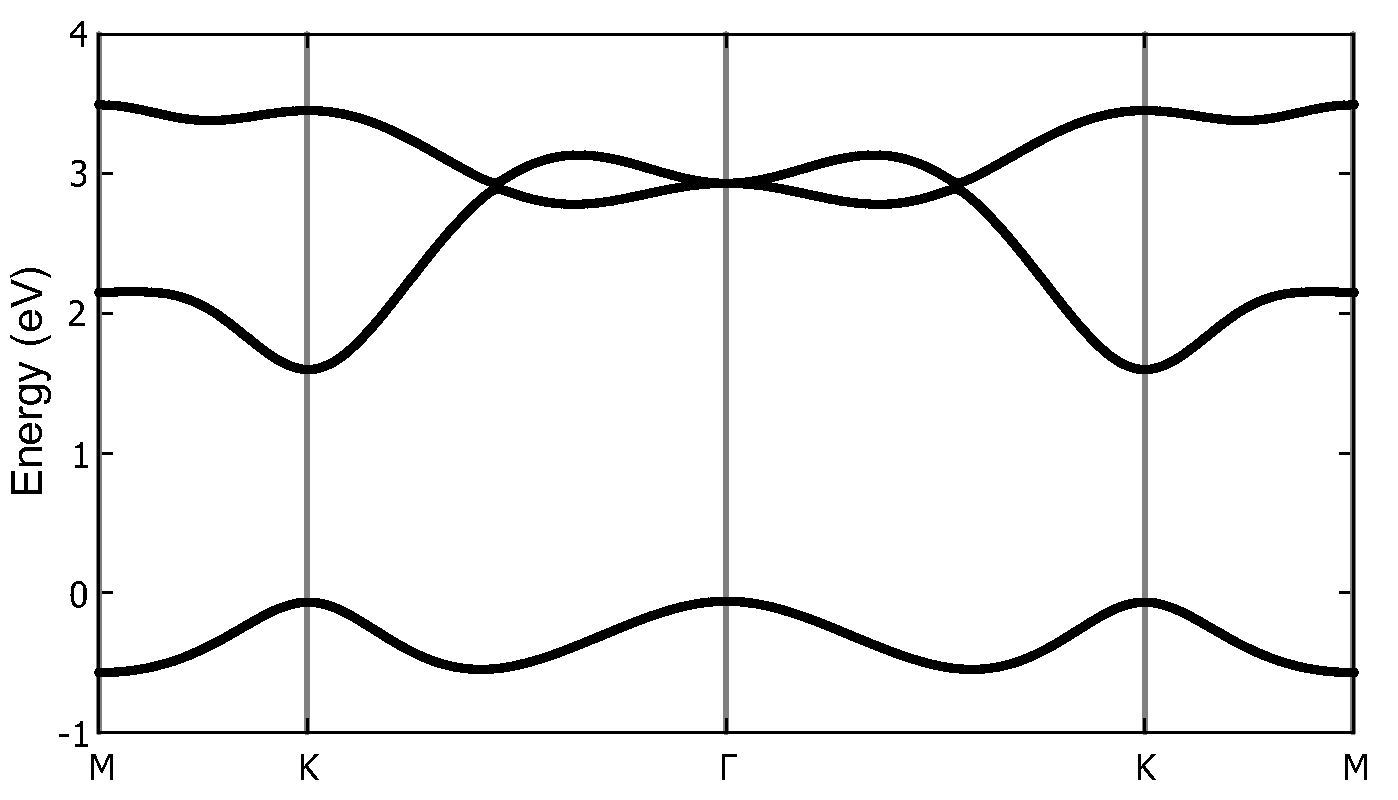
\includegraphics[width=0.75\linewidth]{pic/bandstructure.pdf}
	\caption[Band structure of $\mathrm{MoS}_2$ material along $\Gamma$-K direction]{\label{band structure}To obtain the band structure of monolayer MoS$_{2}$, the eigenvalue of the Hamiltonian needs to be found at each $k$ point across the entire the \ac{BZ}. This figure illustrates the band structure along $\Gamma$-K direction using (GGA) fitting parameters.}
\end{figure*}
\section{Three-band tight binding method under a magnetic field}\label{Section 2.2}
Under a uniform magnetic field given by a vector potential $\mathbf{A}(\mathbf{r})$ the single electron Hamiltonian changes into
\begin{gather}
	H = \f{\left(-i\hbar \boldsymbol{\nabla} + e \mathbf{A(r)}\right)^{2}}{2m} + U_{0}(\mathbf{r}) + g^{*} \mu_{B} \mathbf{B} \cdot \mathbf{L},
\end{gather}
where $\mu_{B} = \f{e\hbar}{2m}$ is Bohr magneton, $g^{*}$ is an effective Landé g-factor, $\mathbf{B} = \boldsymbol{\nabla} \times  \mathbf{A}$ is the uniform magnetic field, and $\mathbf{L}$ is the angular momentum. It is possible to add a phase factor to the tight binding wavefunction
\begin{align}
	\psi_{\lambda,\mathbf{k}} (\mathbf{r}) = \sum_{j=1}^{3} C_{j}^{\lambda}(\mathbf{k}) \sum_{\mathbf{R}} e^{i\mathbf{k \cdot R}} e^{ \theta_{\mathbf{R}}(\mathbf{r})} \phi_{j}(\mathbf{r} - \mathbf{R}).
\end{align}
We now have
\begin{align}
	H_{j j'} (\mathbf{k}) = H_{jj'}^{\text{NN}}(\mathbf{k}) + H_{jj'}^{Z}(\mathbf{k}),
\end{align}
where
\begin{equation}
	\begin{aligned}
		H_{jj'}^{\text{NN}}(\mathbf{k})
		 & = \sum_{\mathbf{R}} \bra{\phi_{j}(\mathbf{r})} e^{-i \theta_{\mathbf{0}}(\mathbf{r})} \left[\f{(-i\hbar \boldsymbol{\nabla} + e \mathbf{A}(\mathbf{r}))^{2}}{2m} + U_{0}(\mathbf{r}) \right] e^{i\mathbf{k \cdot R}} e^{ \theta_{\mathbf{R}}(\mathbf{r})} \ket{\phi_{j'}(\mathbf{r - R})}                        \\
		 & = \sum_{\mathbf{R}} \bra{\phi_{j}(\mathbf{r})} e^{i(\mathbf{k \cdot R} +\theta_{\mathbf{R}} - \theta_{\mathbf{0}} )} \left[ \f{ \left( -i\hbar \boldsymbol{\nabla} + e \mathbf{A} + \hbar \boldsymbol{\nabla} \theta_{\mathbf{R}} \right)^{2} }{2m} + U_{0}(\mathbf{r}) \right] \ket{\phi_{j'}(\mathbf{r - R})},
	\end{aligned}
\end{equation}
and
\begin{align}
	H_{jj'}^{Z}(\mathbf{k})
	 & = g^{*} \mu_{B} \mathbf{B} \cdot \sum_{\mathbf{R}} \bra{\phi_{j}(\mathbf{r})} e^{i(\mathbf{k \cdot R} + \theta_{\mathbf{R}} - \theta_{\mathbf{0}} )} \mathbf{L} \ket{\phi_{j'}(\mathbf{r - R})}.
\end{align}
By choosing $\theta_{\mathbf{R}} = - \f{e}{\hbar} \int_{\mathbf{R}}^{\mathbf{r}} \mathbf{A(\mathbf{r'})} \cdot d\mathbf{r'}$ as Peierls substitution, the Hamiltonian in Eq. (2.25) now reads
\begin{equation}
	\begin{aligned}
		H_{jj'}^{\text{NN}}(\mathbf{k})
		 & = \sum_{\mathbf{R}} \bra{\phi_{j}(\mathbf{r})} e^{i\mathbf{k \cdot R} - \frac{ie}{\hbar} \int_{\mathbf{R}}^{\mathbf{r}} \mathbf{A}(\mathbf{r'}) \cdot d\mathbf{r'} + \frac{ie}{\hbar}\int_{\mathbf{0}}^{\mathbf{r}}\mathbf{A(\mathbf{r'})}\cdot d\mathbf{r'} } \left[- \f{\hbar^{2} \boldsymbol{\nabla}^{2}}{2m} + U_{0} (\mathbf{r}) \right] \ket{\phi_{j'}(\mathbf{r - R})} \nonumber \\
		 & = \sum_{\mathbf{R}}  e^{i\mathbf{k \cdot R}} e^{\frac{ie}{\hbar} \int_{\mathbf{0}}^{\mathbf{R}} \mathbf{A(\mathbf{r'})} \cdot d \mathbf{r'} } \bra{\phi_{j}(\mathbf{r})} e^{-\frac{ie}{\hbar} \Phi_{\mathbf{R,r,0}}} \left[ -\f{\hbar^{2} \boldsymbol{\nabla}^{2}}{2m} + U_{0} (\mathbf{r}) \right] \ket{\phi_{j'}(\mathbf{r - R})},
	\end{aligned}
\end{equation}
where $\Phi_{\mathbf{R,r,0}} = \oint_{\mathbf{R,r,0}} \mathbf{A(\mathbf{r'})} \cdot d\mathbf{r'} $ is the closed loop line integral of $\mathbf{A}$ along the triangle points $\mathbf{R,r,0}$, and $\int_{\mathbf{0}}^{\mathbf{R}} \mathbf{A(\mathbf{r'})} \cdot d \mathbf{r'}$ is the path integral along the two points $\mathbf{R,0}$. Besides that, we have used the fact that
\begin{align}
	\int_{\mathbf{R}}^{\mathbf{r}} \mathbf{A(\mathbf{r'})} \cdot d\mathbf{r'} + \int_{\mathbf{r}}^{\mathbf{0}} \mathbf{A(r')} \cdot \mathbf{r'} = \Phi_{\mathbf{R,r,0}} - \int_{\mathbf{0}}^{\mathbf{R}} \mathbf{A(\mathbf{r'})} \cdot d \mathbf{r'}.
\end{align}
We can show that the flux term $\Phi_{\mathbf{R,r,0}}$ is negligibly small \cite{yalcin_2019} by two observations. When $\mathbf{r}$ is far away from the lattice points $\mathbf{R}$ and $\mathbf{0}$, the flux is large but since the atomic orbitals are highly localized at these two lattice points, the value of the hopping term is very small and the whole hopping term goes to zero. While $\mathbf{r}$ is at or near any of these lattice points, the triangle formed is small, and assuming small magnetic field, the flux term $\Phi_{\mathbf{R,r,0}}$ goes to zero, which giving us the Hamiltonian as
\begin{gather}
	H_{jj'}^{\text{NN}}(\mathbf{k})
	= \sum_{\mathbf{R}} e^{i\mathbf{k \cdot R}}e^{\frac{ie}{\hbar} \int_{\mathbf{0}}^{\mathbf{R}} \mathbf{A(\mathbf{r'})} \cdot d \mathbf{r'} } \bra{\phi_{j}(\mathbf{r})} \left[ -\f{\hbar^{2} \boldsymbol{\nabla}^{2}}{2m} + U_{0} (\mathbf{r}) \right] \ket{\phi_{j'}(\mathbf{r - R})},\\
	H_{jj'}^{Z}(\mathbf{k})
	= g^{*} \mu_{B} \mathbf{B} \cdot \sum_{\mathbf{R}} e^{i\mathbf{k \cdot R}}e^{\frac{ie}{\hbar} \int_{\mathbf{0}}^{\mathbf{R}} \mathbf{A(\mathbf{r'})} \cdot d \mathbf{r'}} \bra{\phi_{j}(\mathbf{r})} \mathbf{L} \ket{\phi_{j'}(\mathbf{r - R})}.
\end{gather}
Considering only \ac{NN} hopping, Eq (2.29) becomes
\begin{equation}
	\begin{aligned}
		H_{jj'}^{\text{NN}}(\mathbf{k})
		 & = \sum_{\mathbf{R}} e^{i\mathbf{k\cdot R}} e^{\frac{e}{\hbar}\int_{0}^{\mathbf{R}}A(\mathbf{r'})d\mathbf{r'}} \mathcal{E}_{jj'}(\mathbf{R})                                                                                                                                                 \\
		 & = \mathcal{E}_{jj'}(\mathbf{0}) + e^{i\mathbf{k\cdot}\mathbf{R}_{1} }e^{\frac{e}{\hbar}\int_{0}^{\mathbf{R}_{1}}A(\mathbf{r'})d\mathbf{r'}} \mathcal{E}_{jj'}(\mathbf{R}_{1})                                                                                                               \\
		 & + e^{i\mathbf{k\cdot}\mathbf{R}_{2} }e^{\frac{e}{\hbar}\int_{0}^{\mathbf{R}_{2}}A(\mathbf{r'})d\mathbf{r'}} \mathcal{E}_{jj'}(\mathbf{R}_{2}) + e^{i\mathbf{k\cdot}\mathbf{R}_{3} }e^{\frac{e}{\hbar}\int_{0}^{\mathbf{R}_{3}}A(\mathbf{r'})d\mathbf{r'}} \mathcal{E}_{jj'}(\mathbf{R}_{3}) \\
		 & + e^{i\mathbf{k\cdot}\mathbf{R}_{3} }e^{\frac{e}{\hbar}\int_{0}^{\mathbf{R}_{3}}A(\mathbf{r'})d\mathbf{r'}} \mathcal{E}_{jj'}(\mathbf{R}_{4}) + e^{i\mathbf{k\cdot}\mathbf{R}_{5} }e^{\frac{e}{\hbar}\int_{0}^{\mathbf{R}_{5}}A(\mathbf{r'})d\mathbf{r'}} \mathcal{E}_{jj'}(\mathbf{R}_{5}) \\
		 & + e^{i\mathbf{k\cdot}\mathbf{R}_{6} }e^{\frac{e}{\hbar}\int_{0}^{\mathbf{R}_{6}}A(\mathbf{r'})d\mathbf{r'}} \mathcal{E}_{jj'}(\mathbf{R}_{6}).
	\end{aligned}
\end{equation}

In the presence of a perpendicular magnetic field $\mathbf{B} \hat{z}$ applied to the plane of \ac{TMD}, we choose the vector potential in the Landau gauge as $\mathbf{A} = (0, Bx, 0)$. For convenience, let us define a shorthand notation for these extra terms 
\begin{equation}
	\begin{aligned}
		\theta_{m,n}^{m',n'}
		 & = \frac{e}{\hbar} \int_{m,n}^{m',n'} \mathbf{A}(\mathbf{r}) \cdot d\mathbf{r} \\
		 & = \frac{eB}{2\hbar}(x_{m} + x_{m'})(y_{n'} - y_{n}),
	\end{aligned}
\end{equation}
in which $x_{m} = \frac{ma}{2}(m = \pm 1, \pm 2)$ and $y_{n} = \frac{na\sqrt{3}}{2}(n = 0,\pm 1)$ are the \ac{NN} coordinates and $a$ being the lattice constant, are shown in \hyperref[fig:site index]{Fig.(2.3)}. Details of this calculation is given in \hyperref[appendix a]{Appendix A}.
\begin{figure}[H]
	\centering
	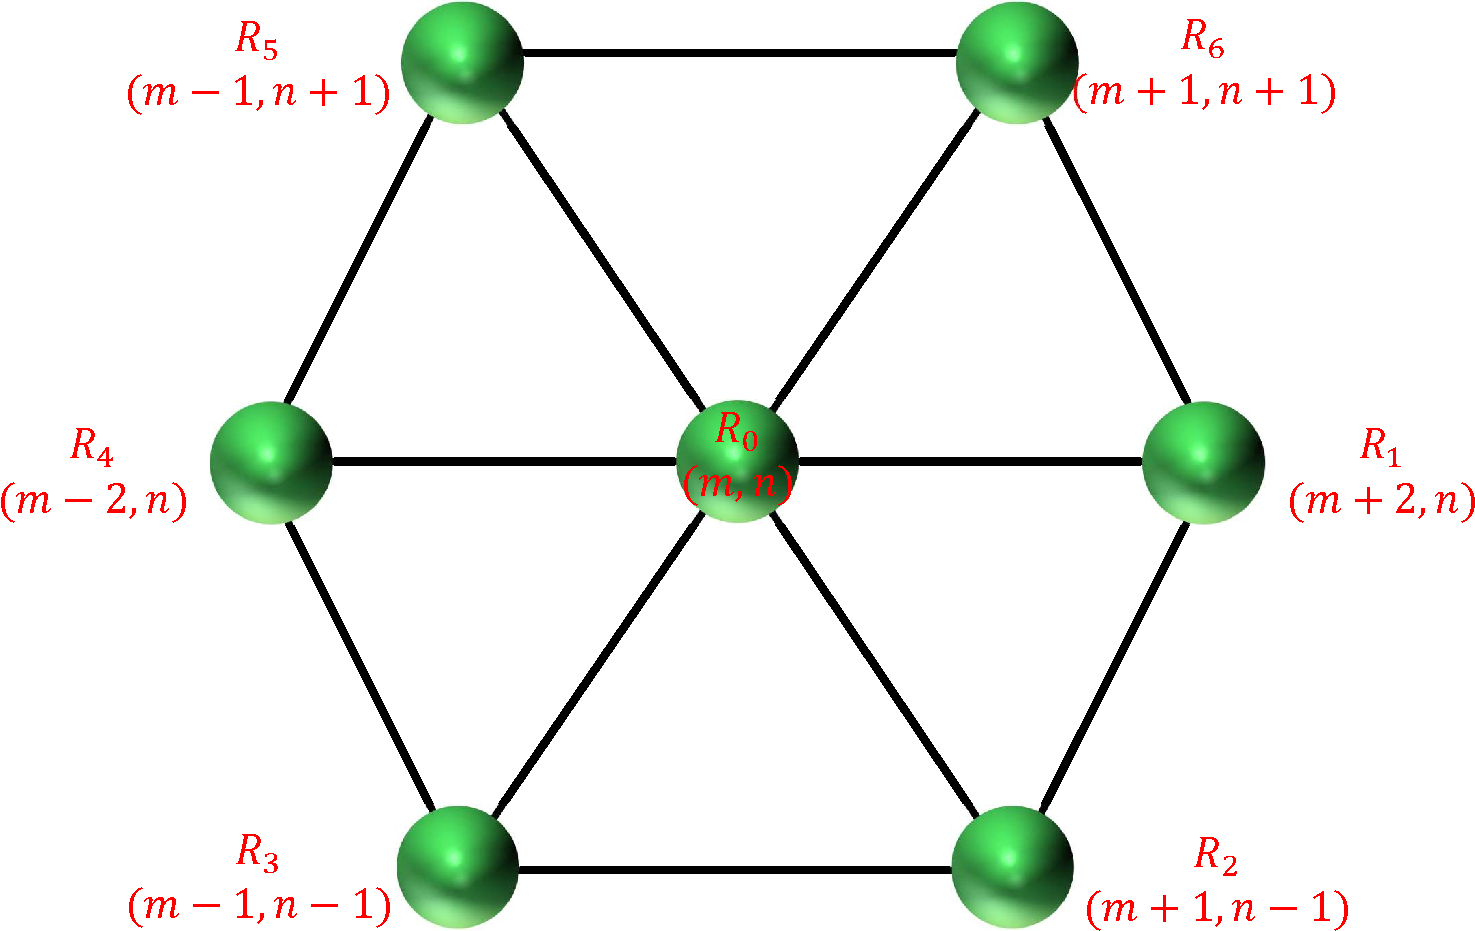
\includegraphics[width=0.85\linewidth]{pic/siteindex_crop.pdf}
	\caption{\label{fig:site index} The \ac{TBM} of \ac{TMD} with six neighbors atom $M$ rewrite with the site index.}
\end{figure}

%In this system, hopping integral of $y$-direction does not change, but hopping integral of $y$-direction change and it depends on the $x$ position.
%Let us now express the Hamiltonian from the zero-field are given by Eq. (2.31) with the transform hopping parameters, noting that the \ac{NN} coordinates are $x = \frac{ma}{2}(m = \pm 1, \pm 2)$ and $y = \frac{na\sqrt{3}}{2}(n = 0,\pm 1)$, $a$ being the lattice constant, are shown in \hyperref[fig:site index]{Fig (2.2)}. 
\noindent Since $dy = 0$ along the $x$ direction, $\theta_{m,n}^{m \pm 2, n} = 0$, and using \ac{NN} coordinates given for lattice site, the $\theta_{m,n}^{m',n'}$ can be written as
\begin{gather}
	\theta_{m,n}^{m',n'} =
	\begin{cases}
		0                                                         & \quad m' = m \pm 2, n' = n  ,    \\
		\pm \frac{e}{\hbar} \frac{B a^{2} \sqrt{3}}{4} (m + 1 /2) & \quad m' = m + 1, n' = n \pm 1 , \\
		\pm \frac{e}{\hbar} \frac{B a^{2} \sqrt{3}}{4} (m - 1 /2) & \quad m' = m - 1, n' = n \pm 1.  \\
	\end{cases}
\end{gather}
Identifying $\frac{B a^{2} \sqrt{3}}{4}$ as the magnetic flux $\Phi$ passing through per unit cell and $\frac{h}{e}$ corresponds to the magnetic flux quantum $\Phi_{0}$, we obtain the following relation:
\begin{equation}
	\begin{aligned}
		H_{jj'}(\mathbf{k})
		 & = E_{jj'}(\mathbf{0}) + e^{i \mathbf{k} \cdot \mathbf{R}_{1}} E_{jj'}(\mathbf{R}_{1}) + e^{-2i\pi(m + 1/2)\Phi / \Phi_{0}} e^{i \mathbf{k} \cdot \mathbf{R}_{2}} E_{jj'}(\mathbf{R}_{2})             \\
		 & + e^{-2i\pi(m - 1/2)\Phi / \Phi_{0}} e^{i \mathbf{k} \cdot \mathbf{R}_{3}} E_{jj'}(\mathbf{R}_{3}) + e^{i \mathbf{k} \cdot \mathbf{R}_{4}} E_{jj'}(\mathbf{R}_{4})                                   \\
		 & + e^{2i\pi(m - 1/2)\Phi / \Phi_{0}} e^{i \mathbf{k} \cdot \mathbf{R}_{5}} E_{jj'}(\mathbf{R}_{5}) + e^{2i\pi(m + 1/2)\Phi / \Phi_{0}} e^{i \mathbf{k} \cdot \mathbf{R}_{6}} E_{jj'}(\mathbf{R}_{6}).
	\end{aligned}
\end{equation}

The Hamiltonian depends only on the site index $m$ and does not invariant under the expansion of a lattice vector along the $x$ axis. In order to restore this invariance, we can look at the case where the ratio of magnetic flux and flux quanta is a rational number $\Phi / \Phi_{0} = p / q$. The crucial advantage of the Peierls phase approach is alowed the lattice periodicity can be restored provided a suitable ``magnetic supercell'' containing several original unit cells is constructed. One might ask what actually happens inside the magnetic unit cells? Do the \ac{NN} still interact in the same way as they did in the tight-binding model? We will focus in this after we get the Hamiltonian for the magnetic unit cell.

The magnetic unit cell has lattice vectors $q\mathbf{a}_{1}$ and $\mathbf{a}_{2}$ is illustrated in Fig.
\begin{figure}[H]
	\centering
	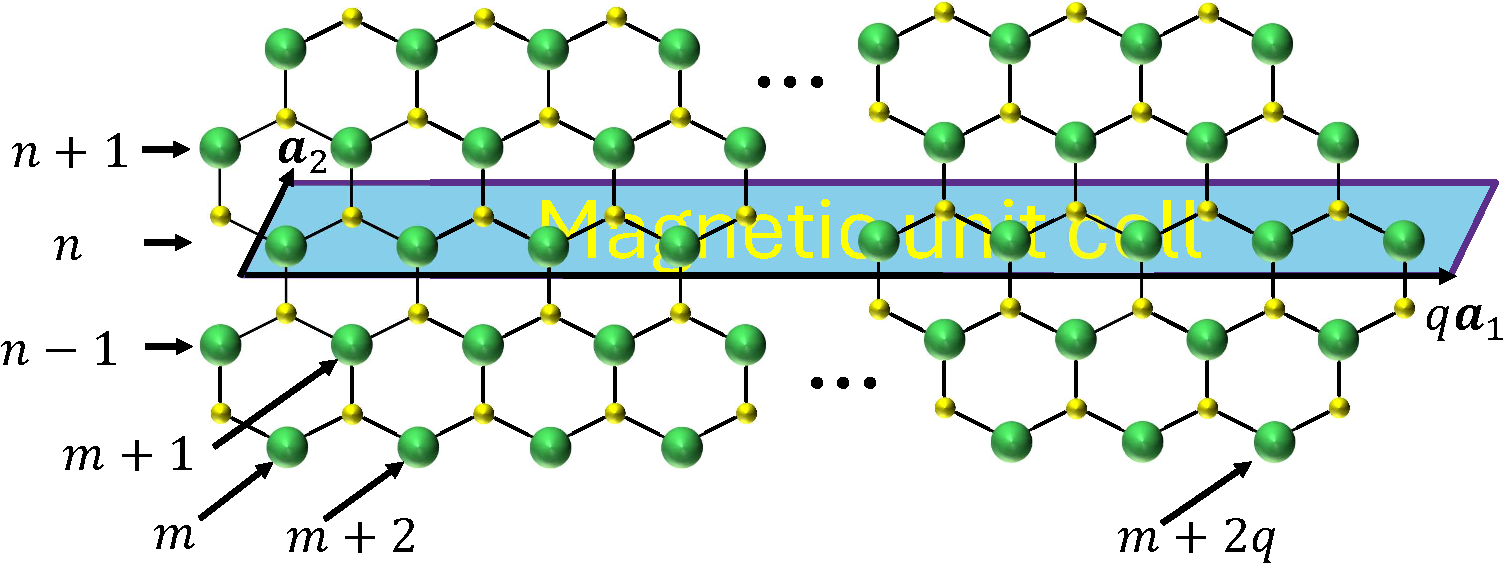
\includegraphics[width=\linewidth]{pic/magneticUC_cut.pdf}
	\caption[Magnetic unit cell for TMD monolayers.]{\label{fig:Mag UC}Magnetic unit cell for TMD monolayers.}
\end{figure}
%Hinh. 

In Section 2.1, we have ignore the sum over of relative positions $\mathbf{r}_{c}$ in Eq (2.2) due to ignore the orbitals of $X$ atoms. While, the magnetic unit cell consits $2q$ atom $M$. We, now, define a new basis set of $6q$ atomic orbitals $\{ \phi_{j}(\mathbf{r} - \mathbf{r}_{i}) \}$ where $j=1,2,3$ and $i = 1,2,...,2q$.
%Here, $\mathbf{r}_{i} = (x_{i},y_{i}) = \frac{ma}{2}\hat{x} + \frac{na\sqrt{3}}{2}\hat{y}$. 
The new basis function now is
\begin{gather}
	\psi_{\lambda,\mathbf{k}}(\mathbf{r}) = \sum_{j,i} C_{ji}^{\lambda}(\mathbf{k}) \sum_{{\alpha}}^{N_{\text{UC}}} e^{i\mathbf{k}\cdot(\mathbf{R}_{\alpha} + \mathbf{r}_{i})} \phi_{j}(\mathbf{r} - \mathbf{R}_{\alpha} - \mathbf{r}_{i}).
\end{gather}
Here, we set $\mathbf{r}_{i}$ refers to the position of an atom in a unit cell, while $\mathbf{R}_{\alpha}$ denotes the position of different unit cells.
The Hamiltonian matrix elements in the new basis is written as
\begin{gather}
	H_{jj'}^{ii'}(\mathbf{k})
	= \sum_{{\alpha}}^{N_\text{UC}}\sum_{{\beta}}^{N_\text{UC}} e^{i \mathbf{k} \cdot (\mathbf{R}_{\beta} - \mathbf{R}_{\alpha} + \mathbf{r}_{i'} - \mathbf{r}_{i})}  \bra{\phi_{j}(\mathbf{r} - \mathbf{R}_{\alpha} - \mathbf{r}_{i})} \left[-\tfrac{\hbar^{2} \boldsymbol{\nabla}^{2}}{2m} + U_{0}\right] \ket{\phi_{j}(\mathbf{r} - \mathbf{R}_{\beta} - \mathbf{r}_{i'})}.
\end{gather}
Now we center our system at $\mathbf{r}'=\mathbf{r} - \mathbf{R}_{\alpha} - \mathbf{r}_{i}$ and define $\mathbf{R}_{\gamma} = \mathbf{R}_{\alpha} - \mathbf{R}_{\beta}$. This leads to
\begin{gather}
	H_{jj'}^{ii'}(\mathbf{k})
	= \sum_{{\alpha}}^{N_\text{UC}}\sum_{{\gamma}}^{N_\text{UC}} e^{-i \mathbf{k} \cdot (\mathbf{R}_{\gamma} + \mathbf{r}_{i} - \mathbf{r}_{i'})}  \bra{\phi_{j}(\mathbf{r})} \left[-\tfrac{\hbar^{2} \boldsymbol{\nabla}^{2}}{2m} + U_{0}\right] \ket{\phi_{j}(\mathbf{r} + \mathbf{R}_{\gamma} + \mathbf{r}_{i} - \mathbf{r}_{i'})}.
\end{gather}
Taking the sum over $\mathbf{R}$ and replacing $\mathbf{r}_{i} = m \mathbf{a}_{1} + n\mathbf{a}_{2} $, $\mathbf{r}_{i'} = m' \mathbf{a}_{1} + n' \mathbf{a}_{2}$, notice that $i = (m,n)$ with only considering the nearest-neighbors, we define our hopping terms in the new basis is given by
\begin{gather}
	H_{ii'}^{jj'}(\mathbf{k}) = \sum_{{\alpha}}^{N_\text{UC}}\sum_{{\gamma}}^{N_\text{UC}} e^{-i \mathbf{k}\cdot \mathbf{R}_{\gamma}} \bra{\phi_{j}(\mathbf{r})} \left[-\f{\hbar^{2} \boldsymbol{\nabla}^{2}}{2m} + U_{0}(\mathbf{r})\right] \ket{\phi_{j'}(\mathbf{r}+\mathbf{R}_{\gamma})}\delta_{i,i'}.
\end{gather}
One can regconize that Eq. (2.37) resembles Eq. (2.6). Additionally, the equation not only describes the hopping between magnetic unit cells but also accounts for hopping between sites within magnetic unit cells. To address the previous question, it is important to note that we have enlarged the original unit cell into a magnetic unit cell, which now contains $2q$ atoms $M$. The \ac{NN} interactions are preserved inside the ``supercell'', but they now involve neighboring magnetic unit cells due to the enlarged cell structure. The Hamiltonian has a discrete tranlastional invariance with a unit cell carrying $2q$ unit cells along the $x$ axis. \\
%e^{\frac{ie}{\hbar} \int_{0}^{r_{i'}+\mathbf{R}} \mathbf{A}(\mathbf{r}')\cdot d\mathbf{r}'}
We can choose $\mathbf{R}_{\beta} = \mathbf{0}$, this will not affect the Hamiltonian because the sum over $\mathbf{R}$ is only considering the \ac{NN} atoms, Hamiltonian with the Peierls phase now is
\begin{equation}
	\begin{aligned}
		& H_{jj'}^{ii'}(\mathbf{k})
		= e^{i\theta_{m,n}^{m,n}}e^{i\mathbf{k} \cdot (\mathbf{0} - \mathbf{0})} \bra{\phi_{j}(\mathbf{r})} \left[-\f{\hbar^{2} \boldsymbol{\nabla}^{2}}{2m} + U_{0}(\mathbf{r})\right] \ket{\phi_{j'}(\mathbf{r})}\delta_{m',m}^{n',n}                               \\
		& + e^{i\theta_{m,n}^{m+2,n}}e^{i\mathbf{k} \cdot (\mathbf{0} - \mathbf{R}_{1})} \bra{\phi_{j}(\mathbf{r})} \left[-\f{\hbar^{2} \boldsymbol{\nabla}^{2}}{2m} + U_{0}(\mathbf{r})\right] \ket{\phi_{j'}(\mathbf{r}-\mathbf{R}_{1})}\delta_{m,m+2}^{n',n}     \\
		& + e^{i\theta_{m,n}^{m-2,n}}e^{i\mathbf{k} \cdot (\mathbf{0} - \mathbf{R}_{4})} \bra{\phi_{j}(\mathbf{r})} \left[-\f{\hbar^{2} \boldsymbol{\nabla}^{2}}{2m} + U_{0}(\mathbf{r})\right] \ket{\phi_{j'}(\mathbf{r}-\mathbf{R}_{4})}\delta_{m',m-2}^{n',n}     \\
		& + e^{i\theta_{m,n}^{m+1,n-1}}e^{i\mathbf{k} \cdot (\mathbf{0} - \mathbf{R}_{2})} \bra{\phi_{j}(\mathbf{r})} \left[-\f{\hbar^{2} \boldsymbol{\nabla}^{2}}{2m} + U_{0}(\mathbf{r})\right] \ket{\phi_{j'}(\mathbf{r}-\mathbf{R}_{2})}\delta_{m',m+1}^{n',n-1} \\
		& + e^{i\theta_{m,n}^{m-1,n-1}}e^{i\mathbf{k} \cdot (\mathbf{0} - \mathbf{R}_{3})} \bra{\phi_{j}(\mathbf{r})} \left[-\f{\hbar^{2} \boldsymbol{\nabla}^{2}}{2m} + U_{0}(\mathbf{r})\right] \ket{\phi_{j'}(\mathbf{r}-\mathbf{R}_{3})}\delta_{m',m-1}^{n',n-1} \\
		& + e^{i\theta_{m,n}^{m-1,n+1}}e^{i\mathbf{k} \cdot (\mathbf{0} - \mathbf{R}_{5})} \bra{\phi_{j}(\mathbf{r})} \left[-\f{\hbar^{2} \boldsymbol{\nabla}^{2}}{2m} + U_{0}(\mathbf{r})\right] \ket{\phi_{j'}(\mathbf{r}-\mathbf{R}_{5})}\delta_{m',m-1}^{n',n+1} \\
		& + e^{i\theta_{m,n}^{m+1,n+1}}e^{i\mathbf{k} \cdot (\mathbf{0} - \mathbf{R}_{6})} \bra{\phi_{j}(\mathbf{r})} \left[-\f{\hbar^{2} \boldsymbol{\nabla}^{2}}{2m} + U_{0}(\mathbf{r})\right] \ket{\phi_{j'}(\mathbf{r}-\mathbf{R}_{6})}\delta_{m',m+1}^{n',n+1}. \\
	\end{aligned}
\end{equation}
Simplizing Eq. (2.38), we get the Hamiltonian for the magnetic unit cell
%\begin{equation}
%	\begin{aligned}
%		& H_{ii'}^{jj'}(\mathbf{k})
%		= \bra{\phi_{j}(\mathbf{r},m,n)} \left[-\tfrac{\hbar^{2}\nabla^{2}}{2m} + U_{0}\right] \ket{\phi_{j}(\mathbf{r},\mathbf{0},m,n)} \delta_{m,m}\delta_{n,n}                                                                                            \\
%		+ & e^{-2i\alpha} e^{i\theta_{m,n}^{m+2,n}} \bra{\phi_{j}(\mathbf{r},m,n)} \left[-\tfrac{\hbar^{2}\nabla^{2}}{2m} + U_{0}\right] \ket{\phi_{j}(\mathbf{r},\mathbf{R}_{1},m,n)}\delta_{m+2,m}\delta_{n,n}                              \\
%		+ & e^{2i\alpha} e^{i\theta_{m,n}^{m-2,n}} \bra{\phi_{j}(\mathbf{r},m,n)} \left[-\tfrac{\hbar^{2}\nabla^{2}}{2m} + U_{0}\right] \ket{\phi_{j}(\mathbf{r},\mathbf{R}_{4},m-2,n)}  \delta_{m-2,m}\delta_{n,n}                          \\
%		+ & e^{i(\alpha - \beta)} e^{i\theta_{m,n}^{m+1,n-1}} \bra{\phi_{j}(\mathbf{r},m,n)} \left[-\tfrac{\hbar^{2}\nabla^{2}}{2m} + U_{0}\right] \ket{\phi_{j}(\mathbf{r},\mathbf{R}_{2},m+1,n-1)}                       \\
%		+ & e^{i(-\alpha - \beta)} e^{i\theta_{m,n}^{m-1,n-1}} \bra{\phi_{j}(\mathbf{r},m,n)} \left[-\tfrac{\hbar^{2}\nabla^{2}}{2m} + U_{0}\right] \ket{\phi_{j}(\mathbf{r},\mathbf{R}_{3},m-1,n-1)}     \\
%		+ & e^{i(-\alpha + \beta)} e^{i\theta_{m,n}^{m-1,n+1}} \bra{\phi_{j}(\mathbf{r},m,n)} \left[-\tfrac{\hbar^{2}\nabla^{2}}{2m} + U_{0}\right] \ket{\phi_{j}(\mathbf{r},\mathbf{R}_{5},m-1,n+1)}                       \\
%		+ & e^{i(\alpha + \beta)} e^{i\theta_{m,n}^{m+1,n+1}} \bra{\phi_{j}(\mathbf{r},m,n)} \left[-\tfrac{\hbar^{2}\nabla^{2}}{2m} + U_{0}\right] \ket{\phi_{j}(\mathbf{r},\mathbf{R}_{6},m+1,n+1)}  . \\
%	\end{aligned}
%\end{equation}
%\begin{equation}
%	\begin{aligned}
%		& H_{ii'}^{jj'}(\mathbf{k})
%		= \bra{\phi_{j}(\mathbf{r} -  m \mathbf{a}_{1} - n\mathbf{a}_{2})} \left[-\frac{\hbar^{2}\nabla^{2}}{2m} + U_{0}\right] \ket{\phi_{j}(\mathbf{r} -  m \mathbf{a}_{1} - n\mathbf{a}_{2})} \delta_{m,m'}^{n,n'}                                                                                                \\
%		+ & e^{i\mathbf{k}\cdot\mathbf{a}_{1}} e^{i\theta_{m,n}^{m',n'}} \bra{\phi_{j}(\mathbf{r} - m \mathbf{a}_{1} - n\mathbf{a}_{2})} \left[-\frac{\hbar^{2}\nabla^{2}}{2m} + U_{0}\right] \ket{\phi_{j}(\mathbf{r} - (m+2) \mathbf{a}_{1} - n\mathbf{a}_{2})} \delta_{m+2,m'}^{n,n'}                             \\
%		+ & e^{-i\mathbf{k}\cdot\mathbf{a}_{1}} e^{i\theta_{m,n}^{m',n'}} \bra{\phi_{j}(\mathbf{r} - m \mathbf{a}_{1} - n\mathbf{a}_{2})} \left[-\frac{\hbar^{2}\nabla^{2}}{2m} + U_{0}\right] \ket{\phi_{j}(\mathbf{r} - (m-2) \mathbf{a}_{1} - n'\mathbf{a}_{2})} \delta_{m-2,m'}^{n,n'}                           \\
%		+ & e^{i\mathbf{k}\cdot\mathbf{a}_{2}} e^{i\theta_{m,n}^{m',n'}} \bra{\phi_{j}(\mathbf{r} - m \mathbf{a}_{1} - n\mathbf{a}_{2})} \left[-\frac{\hbar^{2}\nabla^{2}}{2m} + U_{0}\right] \ket{\phi_{j}(\mathbf{r} - (m+1) \mathbf{a}_{1} - (n+1)\mathbf{a}_{2})} \delta_{m',m+1}^{n',n+1}                       \\
%		+ & e^{i\mathbf{k}\cdot(\mathbf{a}_{2} - \mathbf{a}_{1})} e^{i\theta_{m,n}^{m',n'}} \bra{\phi_{j}(\mathbf{r} - m \mathbf{a}_{1} - n\mathbf{a}_{2})} \left[-\frac{\hbar^{2}\nabla^{2}}{2m} + U_{0}\right] \ket{\phi_{j}(\mathbf{r} - (m-1) \mathbf{a}_{1} - (n+1)\mathbf{a}_{2})} \delta_{m',m-1}^{n',n+1}    \\
%		+ & e^{-i\mathbf{k}\cdot\mathbf{a}_{2}} e^{i\theta_{m,n}^{m',n'}} \bra{\phi_{j}(\mathbf{r} - m \mathbf{a}_{1} - n\mathbf{a}_{2})} \left[-\frac{\hbar^{2}\nabla^{2}}{2m} + U_{0}\right] \ket{\phi_{j}(\mathbf{r} - (m-1) \mathbf{a}_{1} - (n-1)\mathbf{a}_{2})} \delta_{m',m-1}^{n',n-1}                      \\
%		+ & e^{i\mathbf{k}\cdot(-\mathbf{a}_{2} + \mathbf{a}_{1})} e^{i\theta_{m,n}^{m',n'}} \bra{\phi_{j}(\mathbf{r} - m \mathbf{a}_{1} - n\mathbf{a}_{2})} \left[-\frac{\hbar^{2}\nabla^{2}}{2m} + U_{0}\right] \ket{\phi_{j}(\mathbf{r} - (m+1) \mathbf{a}_{1} - (n-1)\mathbf{a}_{2})} \delta_{m',m+1}^{n',n-1} . \\
%	\end{aligned}
%\end{equation}

%Note that $\mathbf{a}_{1} = \mathbf{R}_{1}$, $\mathbf{a}_{2} = \mathbf{R}_{6}$, $-\mathbf{a}_{2} = \mathbf{R}_{3}$, $\mathbf{a}_{2} - \mathbf{a}_{1} = \mathbf{R}_{5}$ and $-\mathbf{a}_{2}+\mathbf{a}_{1} = \mathbf{R}_{2}$.

% Note that
%\begin{gather}
%	\begin{cases}
%		e^{i k_{x} a} \phi_{j} \left(m \frac{a}{2},y\right) = \phi_{j} \left((m+2)\frac{a}{2},y\right),  \\
%		e^{-i k_{x} a} \phi_{j} \left(m\frac{a}{2},y\right) = \phi_{j} \left((m-2)\frac{a}{2},y\right) , \\
%		e^{\pm i k_{x} \frac{a}{2}} e^{\pm i k_{y} \frac{a\sqrt{3}}{2}} \phi_{j} \left(m \frac{a}{2},n \frac{a\sqrt{3}}{2}\right) = e^{\pm i k_{y} \frac{a\sqrt{3}}{2}}\phi_{j} \left((m \pm 1)\frac{a}{2},n\frac{a\sqrt{3}}{2}\right).
%	\end{cases}
%\end{gather}
%Consequently the Hamiltonian matrix in the new basis is written as
%\begin{equation}
%	\begin{aligned}
%		H_{jj'}(\mathbf{k})
%		 & = E_{jj'}(\mathbf{0}) \delta_{m,m} + e^{i\theta_{m,n}^{m',n'}} E_{jj'}(\mathbf{R}_{1}) \delta_{m,m+2} + e^{i\theta_{m,n}^{m',n'}} e^{- i k_{y} \frac{a\sqrt{3}}{2}} E_{jj'}(\mathbf{R}_{2}) \delta_{m,m+1}    \\
%		 & + e^{i\theta_{m,n}^{m',n'}} e^{- i k_{y} \frac{a\sqrt{3}}{2}} E_{jj'}(\mathbf{R}_{3}) \delta_{m,m - 1} + e^{i\theta_{m,n}^{m',n'}} E_{jj'}(\mathbf{R}_{4}) \delta_{m,m + 2}                                  \\
%		 & + e^{i\theta_{m,n}^{m',n'}} e^{i k_{y} \frac{a\sqrt{3}}{2}} E_{jj'}(\mathbf{R}_{5}) \delta_{m,m - 1} + e^{i\theta_{m,n}^{m',n'}} e^{ i k_{y} \frac{a\sqrt{3}}{2}} E_{jj'}(\mathbf{R}_{6}) \delta_{m,m + 1} .
%	\end{aligned}
%\end{equation}

%By substituting Eq (2.32) into Eq (2.35), consequently the Hamiltonian matrix in the new basis is written as
\begin{equation}
	\begin{aligned}
		H_{ii'}^{jj'}(\mathbf{k})
		 & = \mathcal{E}_{jj'}(\mathbf{0}) \delta_{m',m}^{n',n} + e^{-i\mathbf{k} \cdot \mathbf{R}_{1}}\mathcal{E}_{jj'}(\mathbf{R}_{1}) \delta_{m',m+2}^{n',n} + e^{-i\mathbf{k} \cdot \mathbf{R}_{4}}\mathcal{E}_{jj'}(\mathbf{R}_{4})  \delta_{m',m-2}^{n',n}            \\
		 & + e^{-2i\pi(m + 1/2)p / q}e^{-i\mathbf{k} \cdot \mathbf{R}_{2}} \mathcal{E}_{jj'}(\mathbf{R}_{2}) \delta_{m',m+1}^{n',n-1} + e^{-2i\pi(m - 1/2)p / q} e^{-i\mathbf{k} \cdot \mathbf{R}_{3}} \mathcal{E}_{jj'}(\mathbf{R}_{3}) \delta_{m',m-1}^{n',n-1} \\
		 & + e^{2i\pi(m - 1/2)p / q} e^{-i\mathbf{k} \cdot \mathbf{R}_{5}} \mathcal{E}_{jj'}(\mathbf{R}_{5}) \delta_{m',m-1}^{n',n+1} + e^{2i\pi(m + 1/2)p / q} e^{-i\mathbf{k} \cdot \mathbf{R}_{6}} \mathcal{E}_{jj'}(\mathbf{R}_{6}) \delta_{m',m+1}^{n',n+1}.
	\end{aligned}
\end{equation}

Now, for given flux ratio $p/q$, only the $q$ determines the periodicity of the magnetic cell assuming $p$ and $q$ are mutually prime numbers. When we plot the band energies while varying the $p$, we obtain the famous Hofstadter butterfly \cite{PhysRevB.14.2239}, a complex fractal structure as seen in Fig.(2.6). This structure is generated at the $K-$point. This fractal spectrum is a result of two competing effects, lattice periodicity and magnectic unit cell periodicity enforced by the presence of the magnetic field. Eq. (2.39) give the following matrix which must be diagonalized to obtain the energy eigenvalues
\begin{equation}
	\renewcommand{\arraystretch}{0.85}
	\begin{aligned}
		H
		 & =
		\begin{pNiceMatrix}
			h_{0}     & h_{1}      & h_{2}  \\
			h_{1}^{*} & h_{11}     & h_{12} \\
			h_{2}^{*} & h_{12}^{*} & h_{22}
		\end{pNiceMatrix},
	\end{aligned}
\end{equation}
with
\begin{equation}
	\renewcommand{\arraystretch}{0.85}
	\begin{aligned}
		H_{jj'}
		 & =
		\begin{pNiceMatrix}
			\mathcal{E}_{jj'}(\mathbf{0})     & A_{jj'}^{(1)}                     & \mathcal{E}_{jj'}(\mathbf{R}_{1}) & 0                                 & \cdots                            & 0                                 & \mathcal{E}_{jj'}(\mathbf{R}_{4}) & B_{jj'}^{(1)}                     \\
			B_{jj'}^{(2)}                     & \mathcal{E}_{jj'}(\mathbf{0})     & A_{jj'}^{(2)}                     & \mathcal{E}_{jj'}(\mathbf{R}_{1}) & 0                                 & \cdots                            & 0                                 & \mathcal{E}_{jj'}(\mathbf{R}_{4}) \\
			\mathcal{E}_{jj'}(\mathbf{R}_{4}) & B_{jj'}^{(3)}                     & \mathcal{E}_{jj'}(\mathbf{0})     & A_{jj'}^{(3)}                     & \mathcal{E}_{jj'}(\mathbf{R}_{1}) & 0                                 & \cdots                            & 0                                 \\
			\vdots                            & \vdots                            & \vdots                            & \ddots                            & \vdots                            & \vdots                            & \vdots                            & \vdots                            \\
			\mathcal{E}_{jj'}(\mathbf{R}_{1}) & 0                                 & \cdots                            & 0                                 & \mathcal{E}_{jj'}(\mathbf{R}_{4}) & B_{jj'}^{(q-2)}                   & \mathcal{E}_{jj'}(\mathbf{0})     & A_{jj'}^{(q-2)}                   \\
			A_{jj'}^{(q-1)}                   & \mathcal{E}_{jj'}(\mathbf{R}_{1}) & \cdots                            & 0                                 & 0                                 & \mathcal{E}_{jj'}(\mathbf{R}_{4}) & B_{jj'}^{(q-1)}                   & \mathcal{E}_{jj'}(\mathbf{0})     \\
		\end{pNiceMatrix},
	\end{aligned}
\end{equation}
where $A_{jj'}^{(m)} = \mathcal{E}_{jj'}(\mathbf{R}_{2})e^{-2i\pi(m+1/2)p/q}e^{-i \mathbf{k}\cdot \mathbf{R}_{2}} + \mathcal{E}_{jj'}(\mathbf{R}_{6})e^{2i\pi(m+1/2)p/q}e^{-i \mathbf{k}\cdot \mathbf{R}_{6}}$, and $B_{jj'}^{(m)} = \mathcal{E}_{jj'}(\mathbf{R}_{3})e^{-2i\pi(m-1/2)p/q}e^{-i
\mathbf{k}\cdot\mathbf{R}_{3}} + \mathcal{E}_{jj'}(\mathbf{R}_{5})e^{2i\pi(m-1/2)p/q}e^{-i\mathbf{k}\cdot \mathbf{R}_{5}}$
and $h_{0},h_{1},h_{2},h_{11},h_{12},h_{22}$ are submatrices of size $3q \times 3q$. (A visualization is shown in Fig. (2.5))
\begin{figure*}[htb]
	\centering
	\begin{subfigure}[b]{0.495\textwidth}
		\centering
		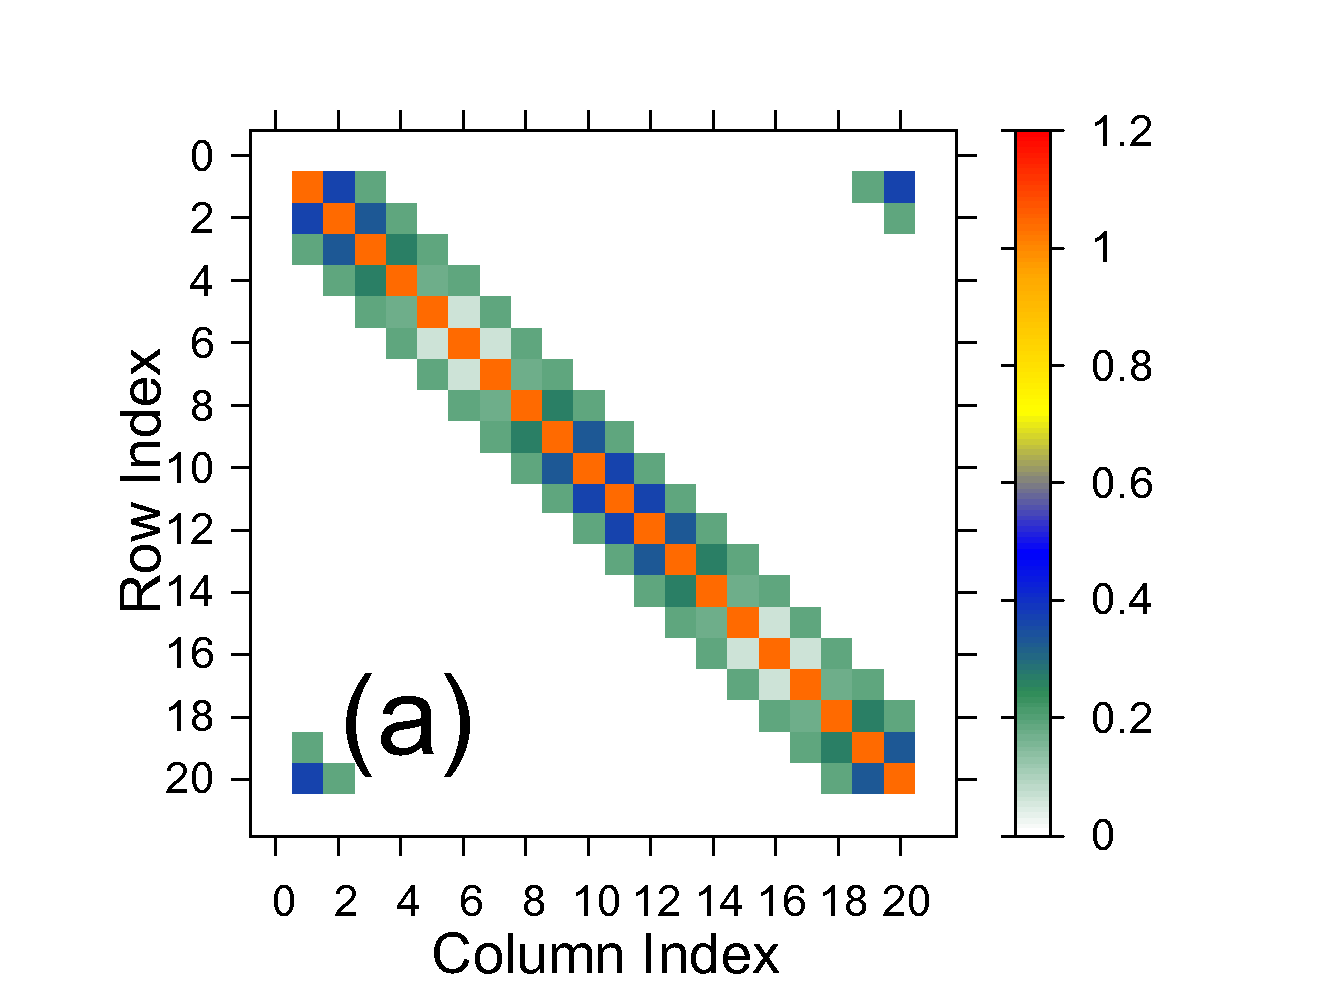
\includegraphics[width=0.9\linewidth]{pic/matrix_1band_h0_q_20.pdf}
		\label{fig:3 band matrix}
	\end{subfigure}
	\begin{subfigure}[b]{0.495\textwidth}
		\centering
		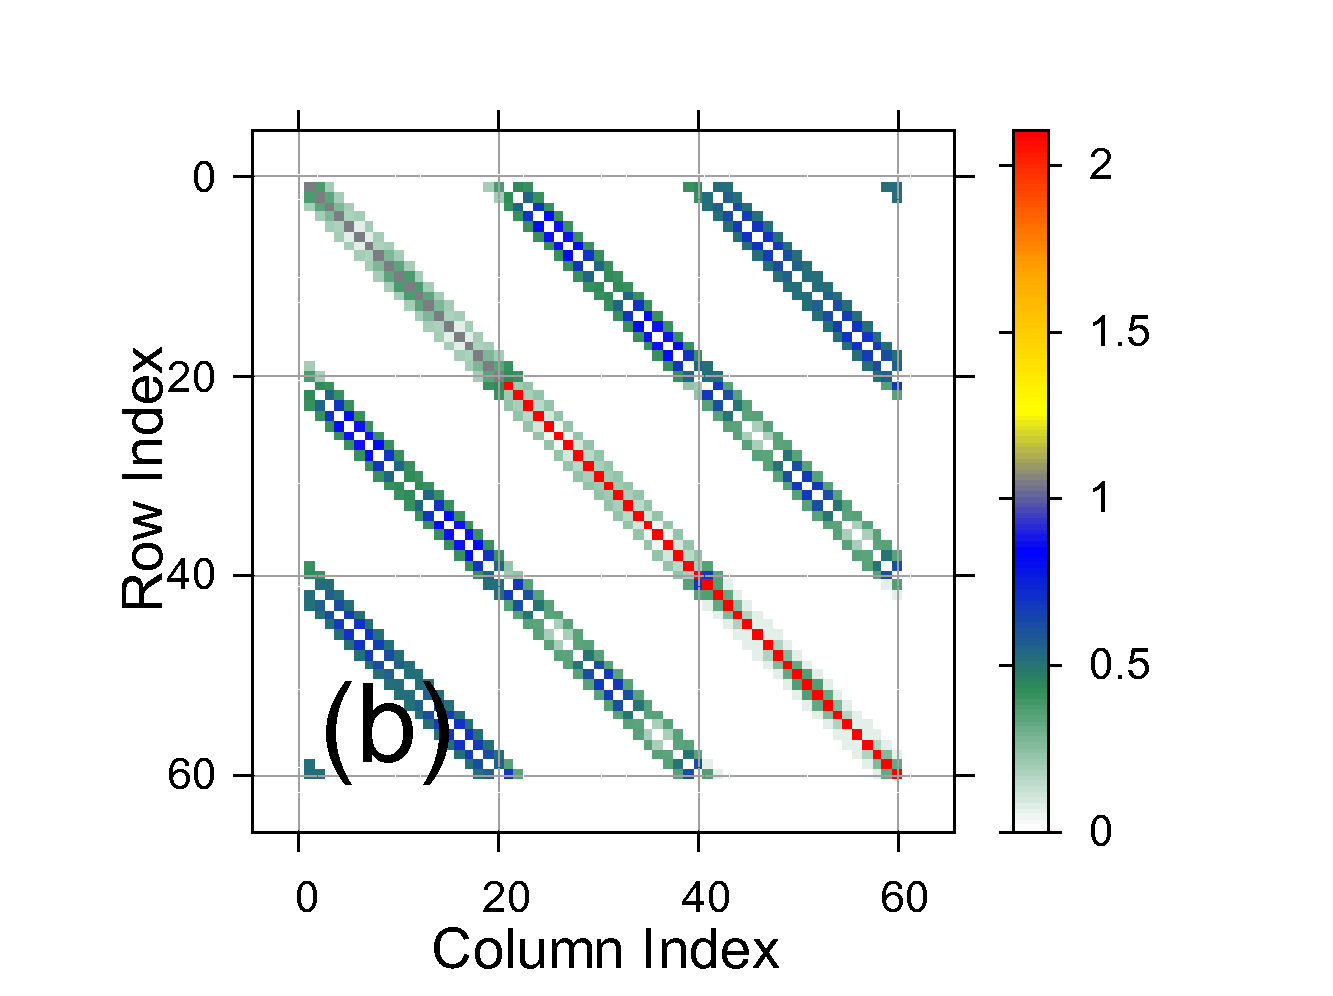
\includegraphics[width=0.9\linewidth]{pic/matrix_3band_h0_q_20.pdf}
		\label{fig:1 band matrix}
	\end{subfigure}
	\caption[A visualization of super matrix.]{
		An simple and intuitive visualization of sub-matrix $h_{0}$ for single-band(a) and matrix $H$ for three band(b) using standard plotter with $q = 20$. (a): orange squares, blue squares and green squares correspond to $\epsilon_{1}, 2 t_{0} \cos \zeta_{1}, t_{0}$, respectively.
	}
\end{figure*}
\begin{figure*}[htb]
	\centering
	\begin{subfigure}[b]{0.495\textwidth}
		\centering
		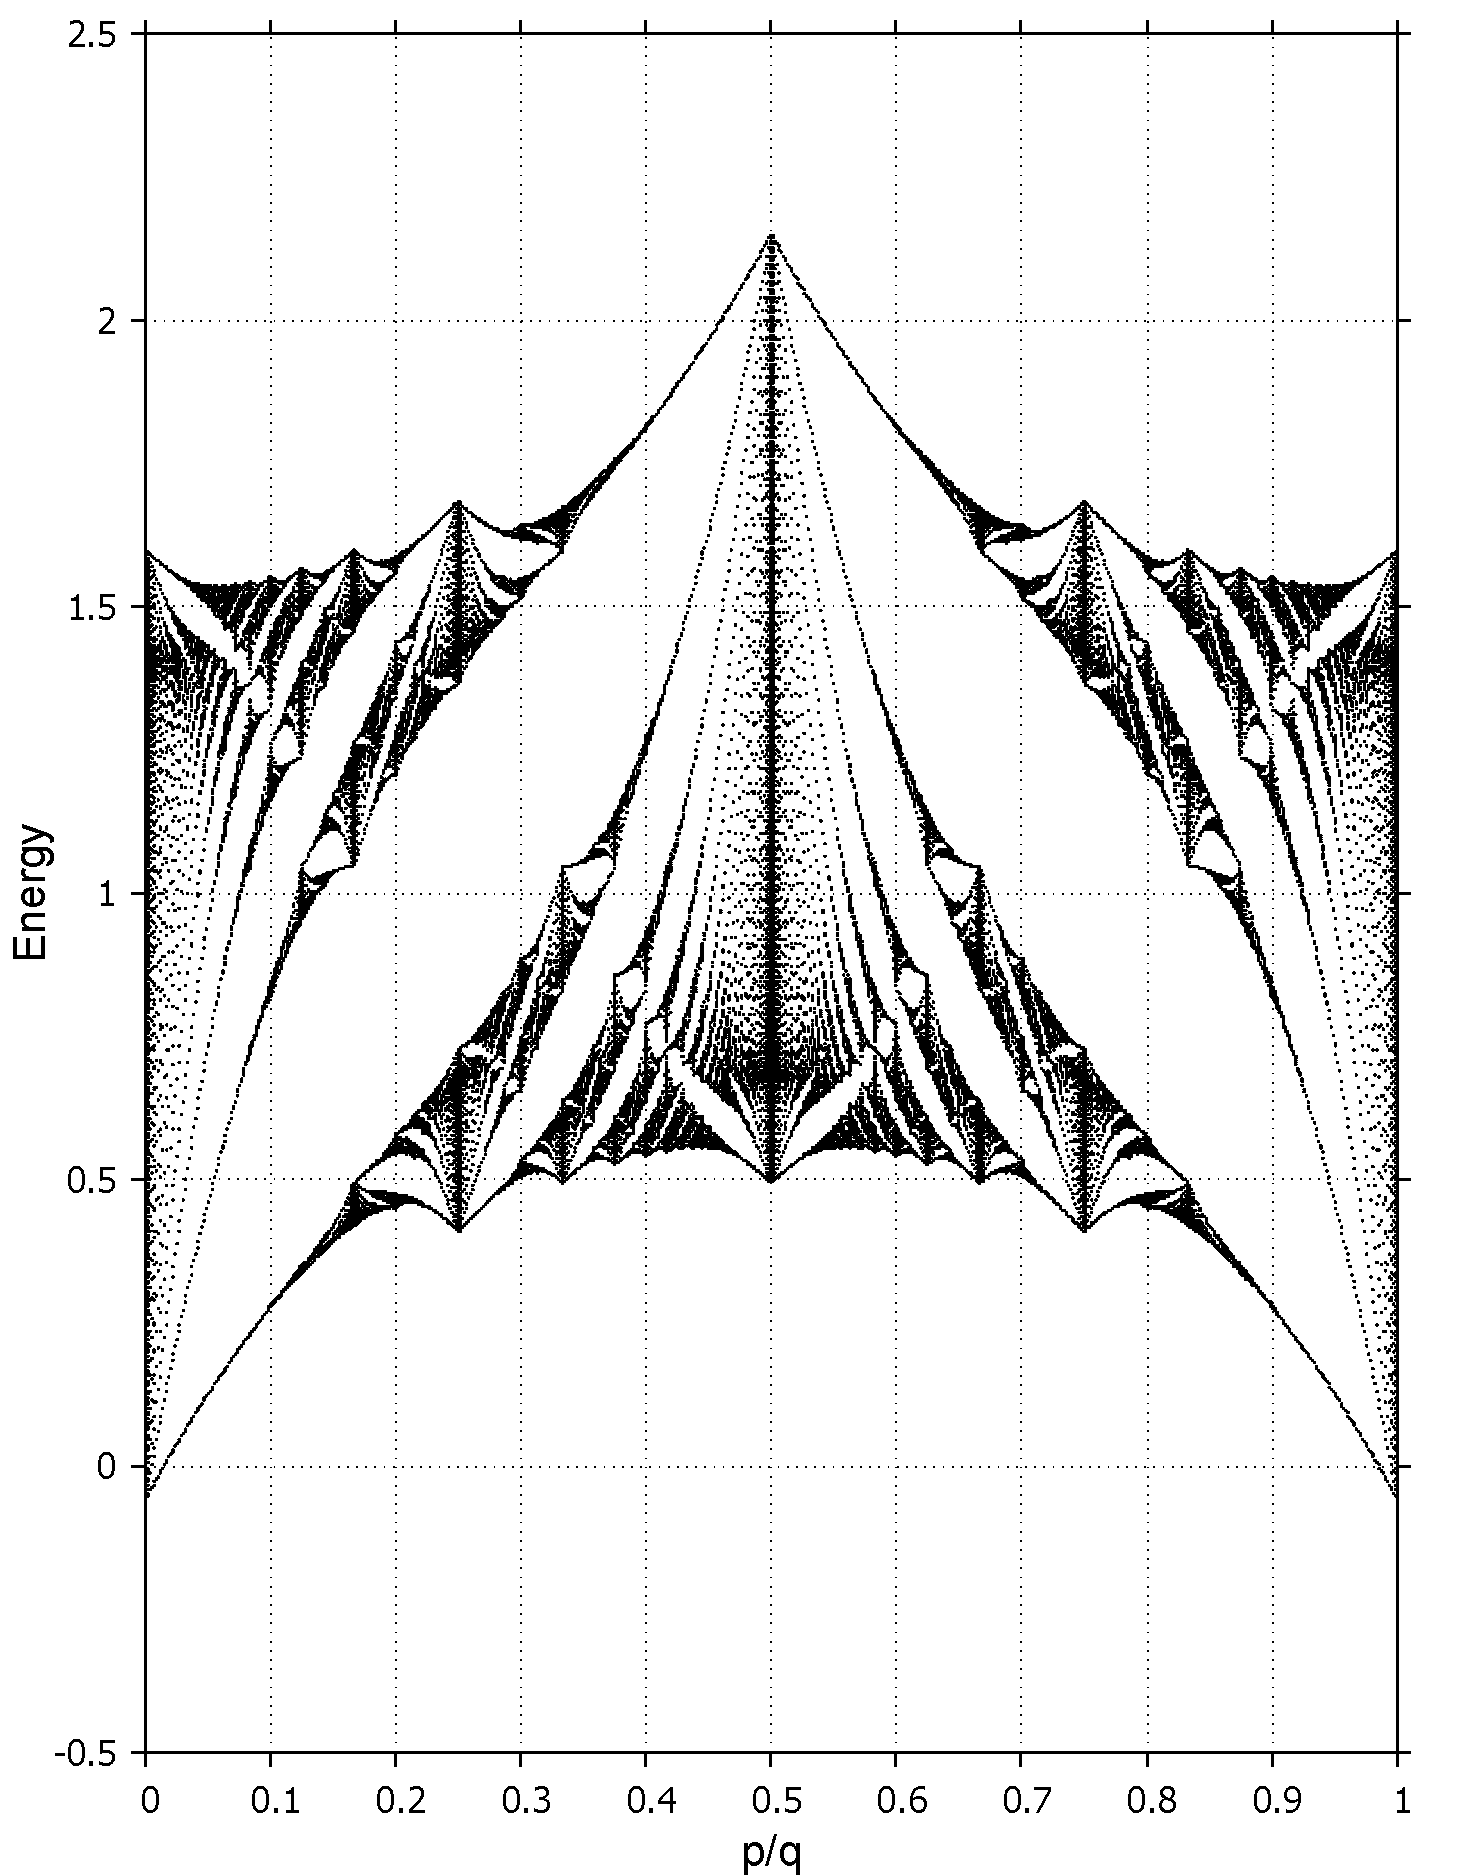
\includegraphics[width=0.85\textwidth,height=1.2\linewidth]{pic/h0_tam giac_q_797.png}
		\label{fig:3 band}
	\end{subfigure}
	\begin{subfigure}[b]{0.495\textwidth}
		\centering
		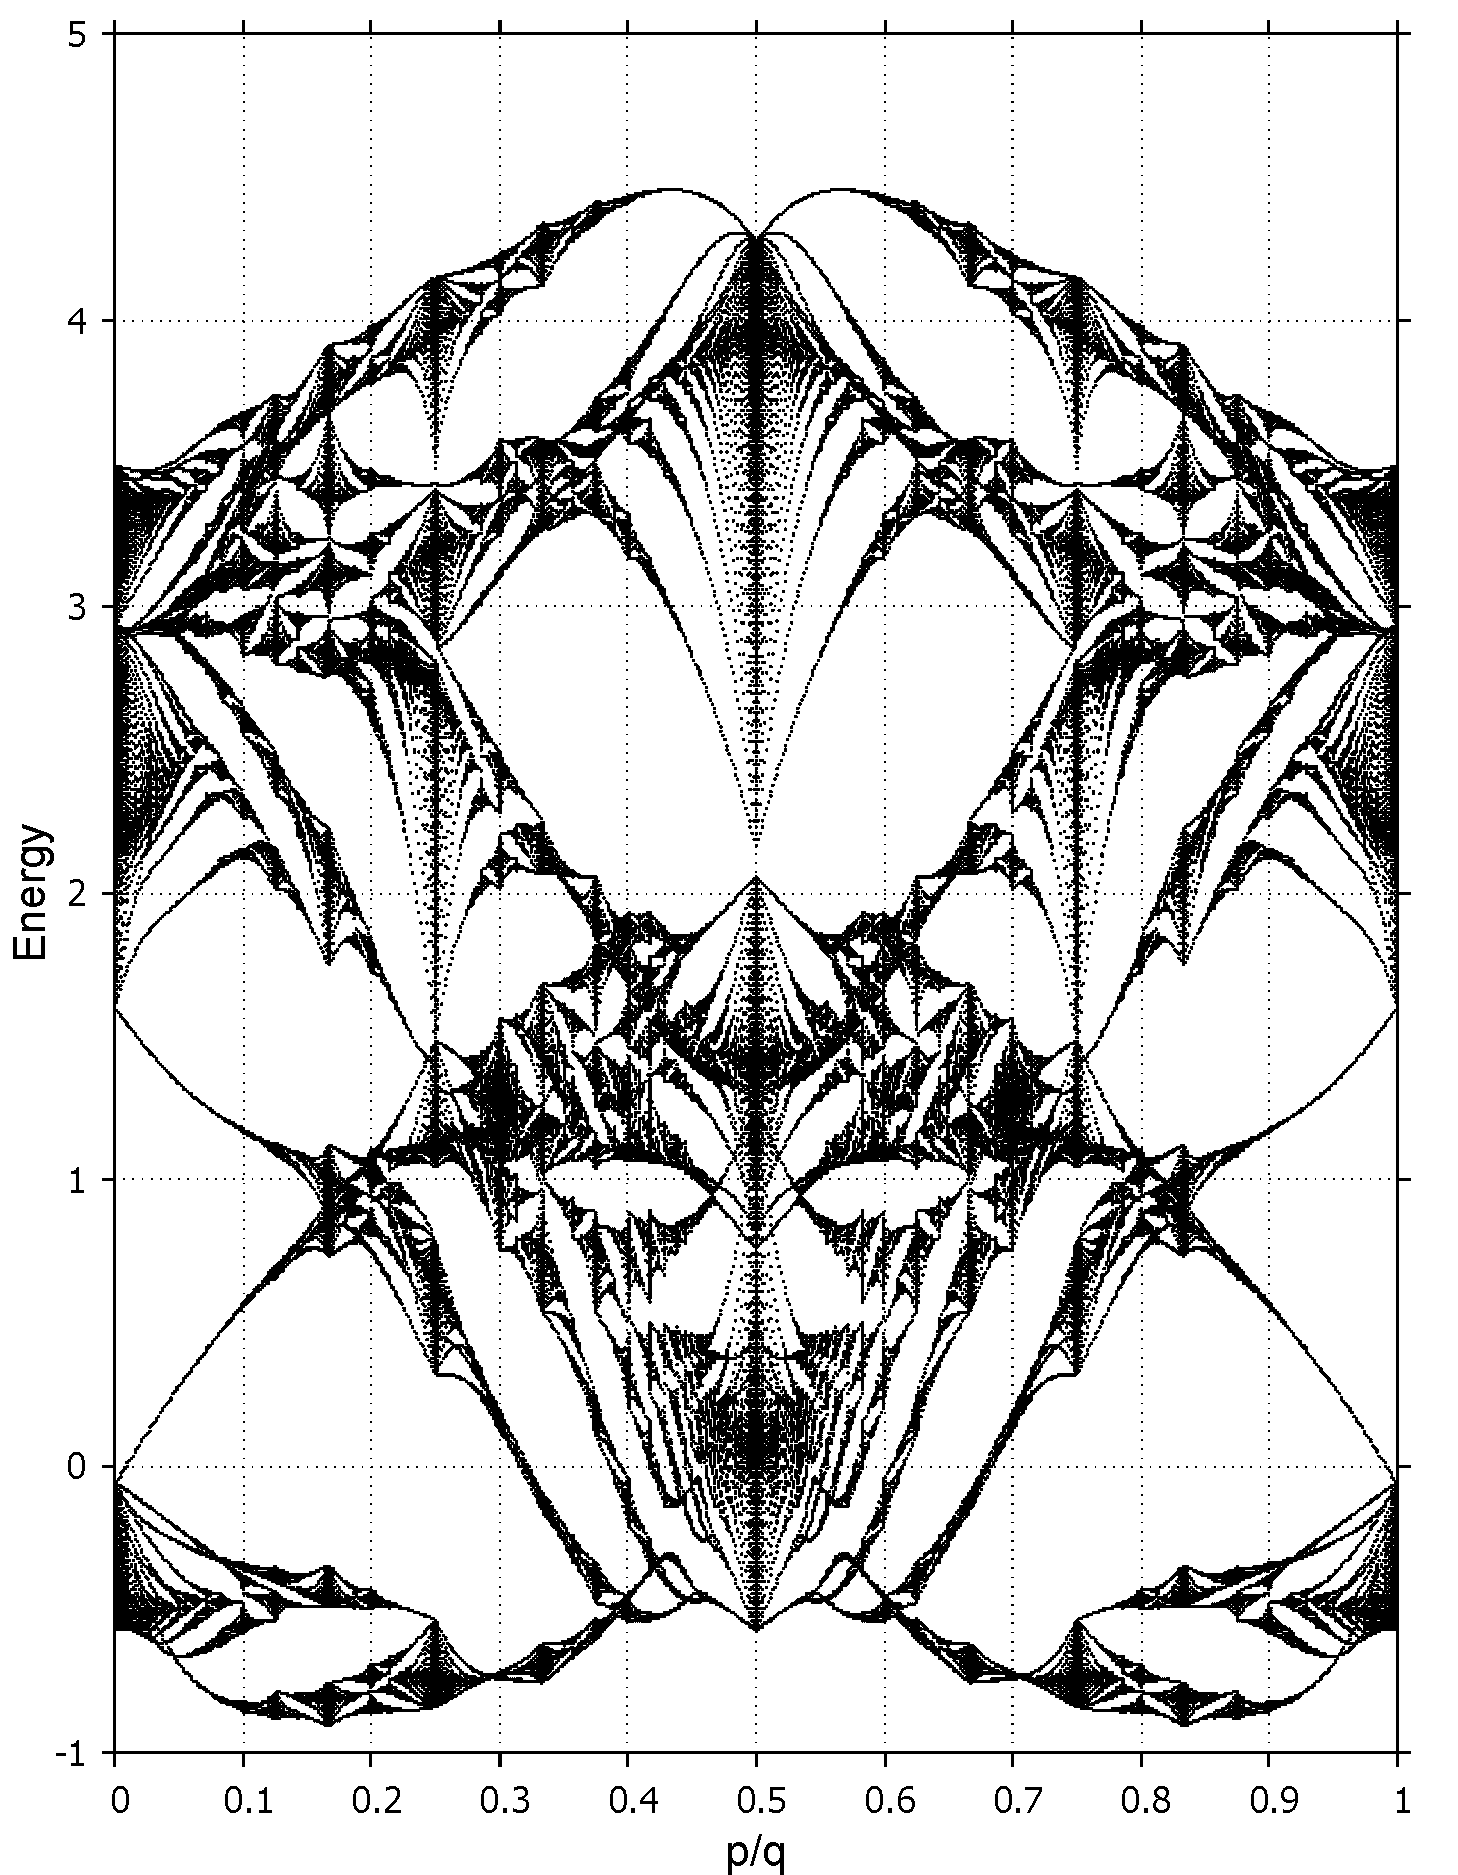
\includegraphics[width=0.85\textwidth,height=1.2\linewidth]{pic/3band_gnuplot_q_797.png}
		\label{fig:1 band}
	\end{subfigure}
	\caption[Hofstadter butterfly for \ac{TMD}.]{
		Hofstadter butterfly for single-band $\ket{dz} \equiv \ket{\phi_{1}^{1}(x,y)}$(left) and all band(right) with $q = 797$ and vary $p$ from 1 to $q$ with field strength $B_{0} = 4.6928 \times 10^{4}$ T. Here on $x-$axis represents the flux in units of quantum flux enclosed by the unit cell and $y-$axis represents the Energy.
	}
\end{figure*}

The magnetic field enters the \ac{TB} Hamiltonian only through the fraction $p/q$, which is the magnetic flux through the primitive unit cell of the lattice. In general, as the lattice geometry evolves, the area of the primitive unit cell changes $m$ times. 

Another observation is that the lattice constant $a$ and the magnetic field $B$ always appears together in an expression with the magnetic field ($\tfrac{Ba^{2}\sqrt{3}}{4}$). This quantity reflects the flux per plaquette in the super magnetic unit cell, which is relevant is the context of Aharonov-Bohm effect \cite{aharonov1959}. Since the expression involves the product $Ba^{2}$, this implies that increasing $B$ by a certain amount is mathematically equivalent to increasing $a$. In other words, for energy calculations, increasing the strength of the magnetic field is physically equivalent to increasing the lattice constant, as both affect the system in the same way through the flux per unit cell.

The spectrum exhibits several notable symmetries. First, it depends only on the flux ratio $p/q$, meaning that shifting $p/q$ by an integer $c$ (i.e., $p/q \rightarrow p/q + c$) leaves the spectrum unchanged. Additionally, the spectrum remains invariant under the transformation $p/q \rightarrow -p/q$, since if $\psi$ is an eigenstate with energy $E$ for flux $p/q$, its complex conjugate $\psi^*$ is an eigenstate with the same energy for flux $-p/q$. These two symmetries are general and not specific to the $MX_{2}$ case. The third symmetry involves changing $p/q$ to $p/q + 1/2$, which is equivalent to flipping the sign of the hopping energies $t_{i}$ (i.e., $t_{i} \rightarrow -t_{i}$), resulting in an inversion of the spectrum.

The role of the eight hopping constants $t$ is just to set an energy scale. Change the hopping constants amounts to stretching the butterfly spectrum vertically, which is an overall scaling to the energy levels. Thus it does not give rise to any interesting physical phenomenon. The three-band spectrum contains a complex and rich physics insight but it seem remains the fractal structure
\begin{figure*}[htb]
	\centering
	\begin{subfigure}[b]{0.32\linewidth}
		\centering
		\includegraphics[width=0.95\textwidth,height=1.2\linewidth]{pic/plotHofstadterButterfly_q=797_MoS2.png}
		\label{fig:matt 1}
	\end{subfigure}
	\begin{subfigure}[b]{0.32\linewidth}
		\centering
		\includegraphics[width=0.95\textwidth,height=1.2\linewidth]{pic/plotHofstadterButterfly_q=797_MoSe2.png}
		\label{fig:matt 2}
	\end{subfigure}
	\begin{subfigure}[b]{0.32\linewidth}
		\centering
		\includegraphics[width=0.95\textwidth,height=1.2\linewidth]{pic/plotHofstadterButterfly_q=797_MoTe2.png}
		\label{fig:matt 3}
	\end{subfigure}
	\begin{subfigure}[b]{0.32\linewidth}
		\centering
		\includegraphics[width=0.95\textwidth,height=1.2\linewidth]{pic/plotHofstadterButterfly_q=797_WS2.png}
		\label{fig:matt 4}
	\end{subfigure}
	\begin{subfigure}[b]{0.32\linewidth}
		\centering
		\includegraphics[width=0.95\textwidth,height=1.2\linewidth]{pic/plotHofstadterButterfly_q=797_WSe2.png}
		\label{fig:matt 5}
	\end{subfigure}
	\begin{subfigure}[b]{0.32\linewidth}
		\centering
		\includegraphics[width=0.95\textwidth,height=1.2\linewidth]{pic/plotHofstadterButterfly_q=797_WTe2.png}
		\label{fig:matt 6}
	\end{subfigure}
	\caption[Showcase Hofstadter’s butterflies of $MX_{2}$ monolayers.]{
		Hofstadter’s butterflies of $MX_{2}$ monolayers using GGA parameters from Table 1.
	}
\end{figure*}


%Using Eq (2.16), we obtain the eigenvalue equation $H \phi_{\mu}^{j} = E \phi_{\mu}^{j}$ and


% t_{0} e^{- i \left(2  \pi (m + \frac{1}{2}) \eta + k_{y} a \frac{\sqrt{3}}{2}\right) }
%An alternative approach to the derivation of the Hamiltonian under an uniform magnetic field is given in \hyperref[appendix b]{Appendix B}.
%\newpage
%\section{Spin-orbit coupling}
\newpage
Due to the significant mass of the transition-metal atom $M$, its \ac{SOC} can be large. For simplicity, we consider only the on-site contribution, which corresponds to the $\mathbf{L \cdot S}$ term originating from the $M$ atoms. Using the basis set $\left\{\ket{d_{z^{2}},\uparrow},\ket{d_{xy},\uparrow},\ket{d_{x^{2} - y^{2}},\uparrow},\ket{d_{z^{2}},\downarrow},\ket{d_{xy},\downarrow},\ket{d_{x^{2} - y^{2}},\downarrow}\right\}$, we derive the SOC term in the Hamiltonian as
\begin{gather}
	H{'}
	= \lambda \mathbf{L \cdot S}
	= \f{\lambda}{2}
	\begin{pNiceMatrix}
		L_{z}           & L_{x} - i L_{y} \\
		L_{x} + i L_{y} & -L_{z}
	\end{pNiceMatrix},
\end{gather}
in which
\begin{gather}
	L_{z}
	=
	\begin{pNiceMatrix}
		0 & 0   & 0  \\
		0 & 0   & 2i \\
		0 & -2i & 0
	\end{pNiceMatrix},
\end{gather}
is the matrix of $\hat{L}_{z}$ ($z$ component of the orbital angular momentum) in bases of $d_{z^{2}},d_{xy},d_{x^{2} - y^{2}}$ and $\lambda$ is characterized the strength of the \ac{SOC}. Noting that, under the three bases, the matrix elements of $\hat{L}_{x}$ and $\hat{L}_{y}$ are all zeros. Therefore the full \ac{TB} Hamiltonian for the magnetic unit cell with the SOC as follows
\begin{equation}
	\begin{aligned}
		H_{\text{SOC}}(\mathbf{k})
		 & = \mathbf{I}_{2} \otimes H(\mathbf{k}) + \mathbf{I}_{q} \otimes H{'} \\
		 & =
		\begin{pmatrix}
			H_{3q \times 3q}(\mathbf{k}) + \frac{\lambda}{2} L_{z} & 0                                                      \\
			0                                                      & H_{3q \times 3q}(\mathbf{k}) - \frac{\lambda}{2} L_{z}
		\end{pmatrix},
	\end{aligned}
\end{equation}
in which $\mathbf{I}_{2}$ is the $2\times 2$ identity matrix.

%To obtain the band structure, the eigenvalue of the Hamiltonian needs to be found at each


\begin{figure*}[htb]
	\begin{subfigure}[b]{0.495\textwidth}
		\centering
		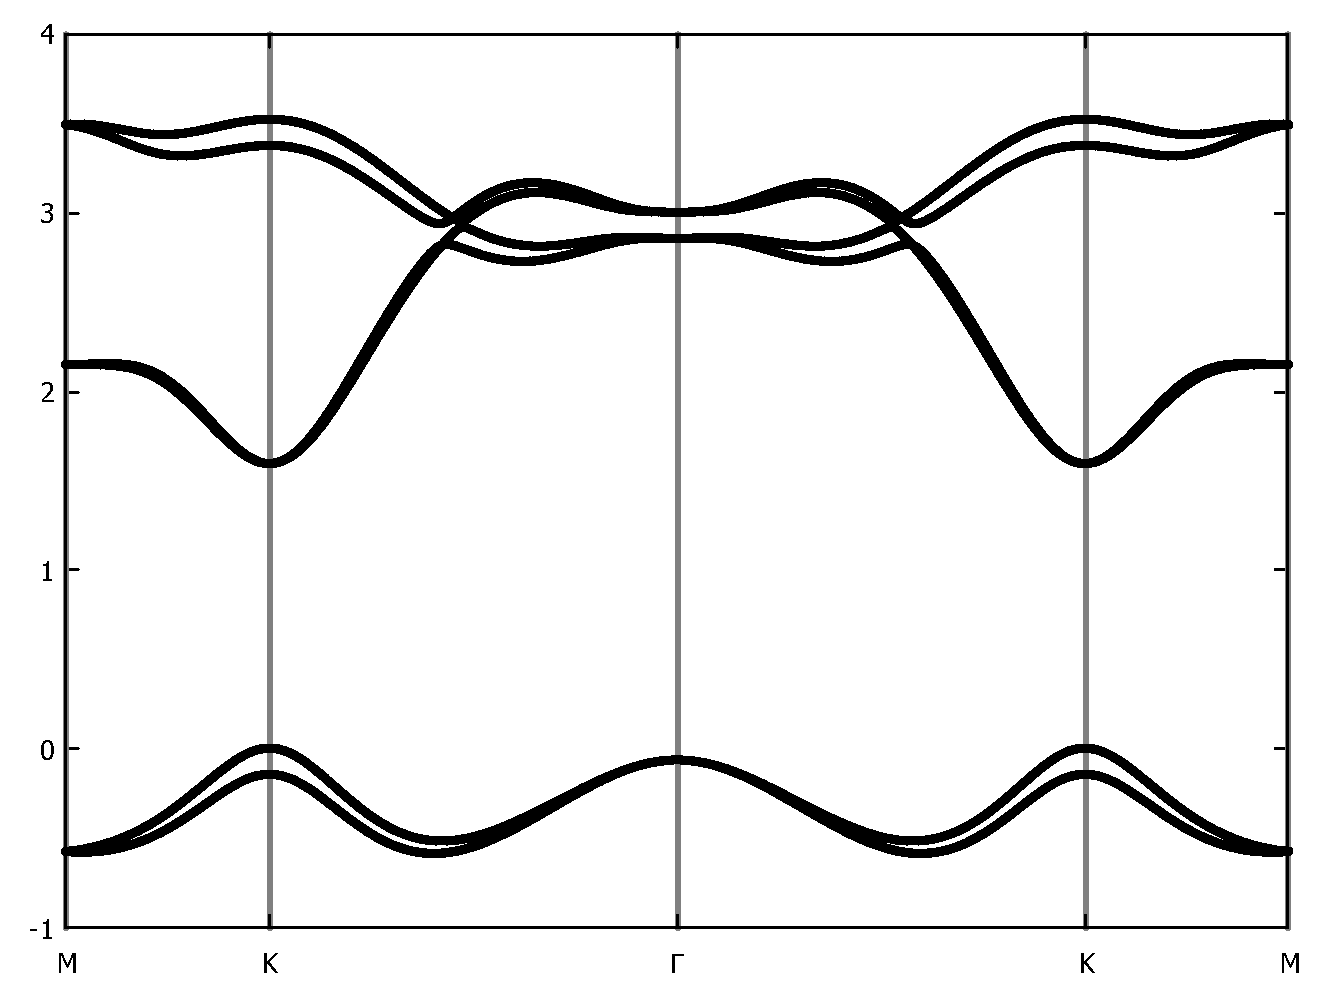
\includegraphics[width=\linewidth]{pic/bandstructureSOC.pdf}
		%\caption{\label{band structure SOC}}
	\end{subfigure}
	\begin{subfigure}[b]{0.495\textwidth}
		\centering
		\includegraphics[width=\linewidth]{pic/plotHofstadterButterfly_q=797_MoS2_SOC.png}
		%\caption{\label{HB SOC}}
	\end{subfigure}
	\caption[Hofstadter butterfly with SOC.]{Band structure of monolayer $MoS_{2}$ along $\Gamma$-K direction, SOC causes huge spin splittings in band-structure at $K$ and $-K$ points.}
\end{figure*}

An alternative approach to the derivation of the Hamiltonian under an uniform magnetic field is given in \hyperref[appendix b]{Appendix A}.

\section{Landau levels}
In solid-state physics, the behavior of electrons in magnetic fields is usually introduced by using the Hamiltonian
\begin{gather}
	H = \f{\mathbf{p} + e \mathbf{A}(\mathbf{r})^{2}}{2m} ,
\end{gather}
and the energy eigenfunctions are known as \ac{LLs}
\begin{gather}
	E_{n} = \left(n + 1/2\right) \hbar \omega_{c}.
\end{gather}

This treatment is for free electrons, but near the bottom of the two-dimensional tight-binding band of \ac{TMD} we must find a regime in which the electron behaves as a nearly one(At least with a nearly free dispersion relation). \\
Recalling the result obtained for the dispersion relation of an electron within the \ac{TBM}
\begin{gather}
	h_{0} = 2 t_{0} (\cos 2\alpha + 2 \cos \alpha \cos \beta) + \epsilon_{1},
\end{gather}
The dispersion energy is approximately free-electron-like by Taylor expansion to second order of $\mathbf{k}$
\begin{equation}
	\begin{aligned}
		h_{0}(\mathbf{k})
		 & \approx 2 t_{0} \left[1 - \frac{a^{2} k_{x}^{2}}{2} + 2\left(1 - \f{a^{2} k_{x}^{2}}{8}\right)\left(1 - \f{3a^{2} k_{y}^{2}}{8}\right)\right] \\
		 & = t_{0} \f{3}{16} \left(32 + a^{4} k_{x}^{2} k_{y}^{2}\right) - t_{0} \f{3}{2} a^{2}\left(k_{x}^{2} + k_{y}^{2}\right) + \epsilon_{1} ,
	\end{aligned}
\end{equation}
the term $a^{4}$ is negligibly small, then we have
\begin{equation}
	\begin{aligned}
		h_{0}(\mathbf{k})
		 & \approx 6 t_{0} - \f{3}{2} t_{0} a^{2} (k_{x}^{2} + k_{y}^{2}) + \epsilon_{1}.
	\end{aligned}
\end{equation}
One of the ways derivation of effective mass $m^{*}$ is substitution $\hbar\mathbf{k} \rightarrow \mathbf{\Pi} + e \mathbf{A}$, with Landau gauge $\mathbf{A} = (0,Bx,0)$
\begin{equation}
	\begin{aligned}
		h_{0}(\mathbf{\Pi})
		 & \approx 6 t_{0} - \f{3}{2} t_{0} \f{a^{2}}{\hbar^{2}} \left[ \Pi_{x}^{2} + \left(\Pi_{y} + e B x\right)^{2}\right] + \epsilon_{1}                                                           \\
		 & \approx 6 t_{0} - \f{3}{2} t_{0} \f{a^{2}}{\hbar^{2}} \Pi_{x}^{2} - \f{3}{2} t_{0} \f{a^{2}}{\hbar^{2}} (e B)^{2} \left[ x - \left(- \f{\hbar k_{y}}{eB}\right) \right]^{2} + \epsilon_{1}.
	\end{aligned}
\end{equation}
The Eq (2.50) can be rewrite in the form as
\begin{gather}
	E(\mathbf{\Pi}) = 6 t_{0} - \left[\f{1}{2m^{*}} \Pi_{x}^{2} + \f{1}{2} m^{*} \omega_{c}^{2}(x - x_{0})^{2}\right] + \epsilon_{1},
\end{gather}
where $m^{*} = \frac{\hbar^{2}}{3t_{0}a^{2}}$ is the effective mass and $x_{0} = \frac{\hbar k_{y}}{eB}$. Subsequently, the cyclotron frequency is
\begin{gather}
	\omega_{c} = \f{eB}{m^{*}} = \f{8 \pi \sqrt{3} t_{0}}{\hbar}  \f{p}{q},
\end{gather}
and therefore the Landau levels near the bottom of the band structure can be written as
\begin{equation}
	\begin{aligned}
		E_{n}
		 & = 6 t_{0} - \hbar \omega_{c} (n + 1 /2) + \epsilon_{1}                    \\
		 & = t_{0} \left(6 - 8\pi\sqrt{3} \f{p}{q}( n + 1 /2)\right) + \epsilon_{1},
	\end{aligned}
\end{equation}
in linear order of an uniform-flux, where $n$ is Landau index. These levels give rise to what is called ``the Landau fan'', being very important in the de Haas-van Alphen and Shubnikov-de Haas effects \cite{10.1119/1.1615568} which predicts oscillations of the magnetic moment of a meltal depending on an applied magnetic field.
\begin{figure*}[htb]
	\centering
	\begin{subfigure}[b]{0.49\textwidth}
		\centering
		{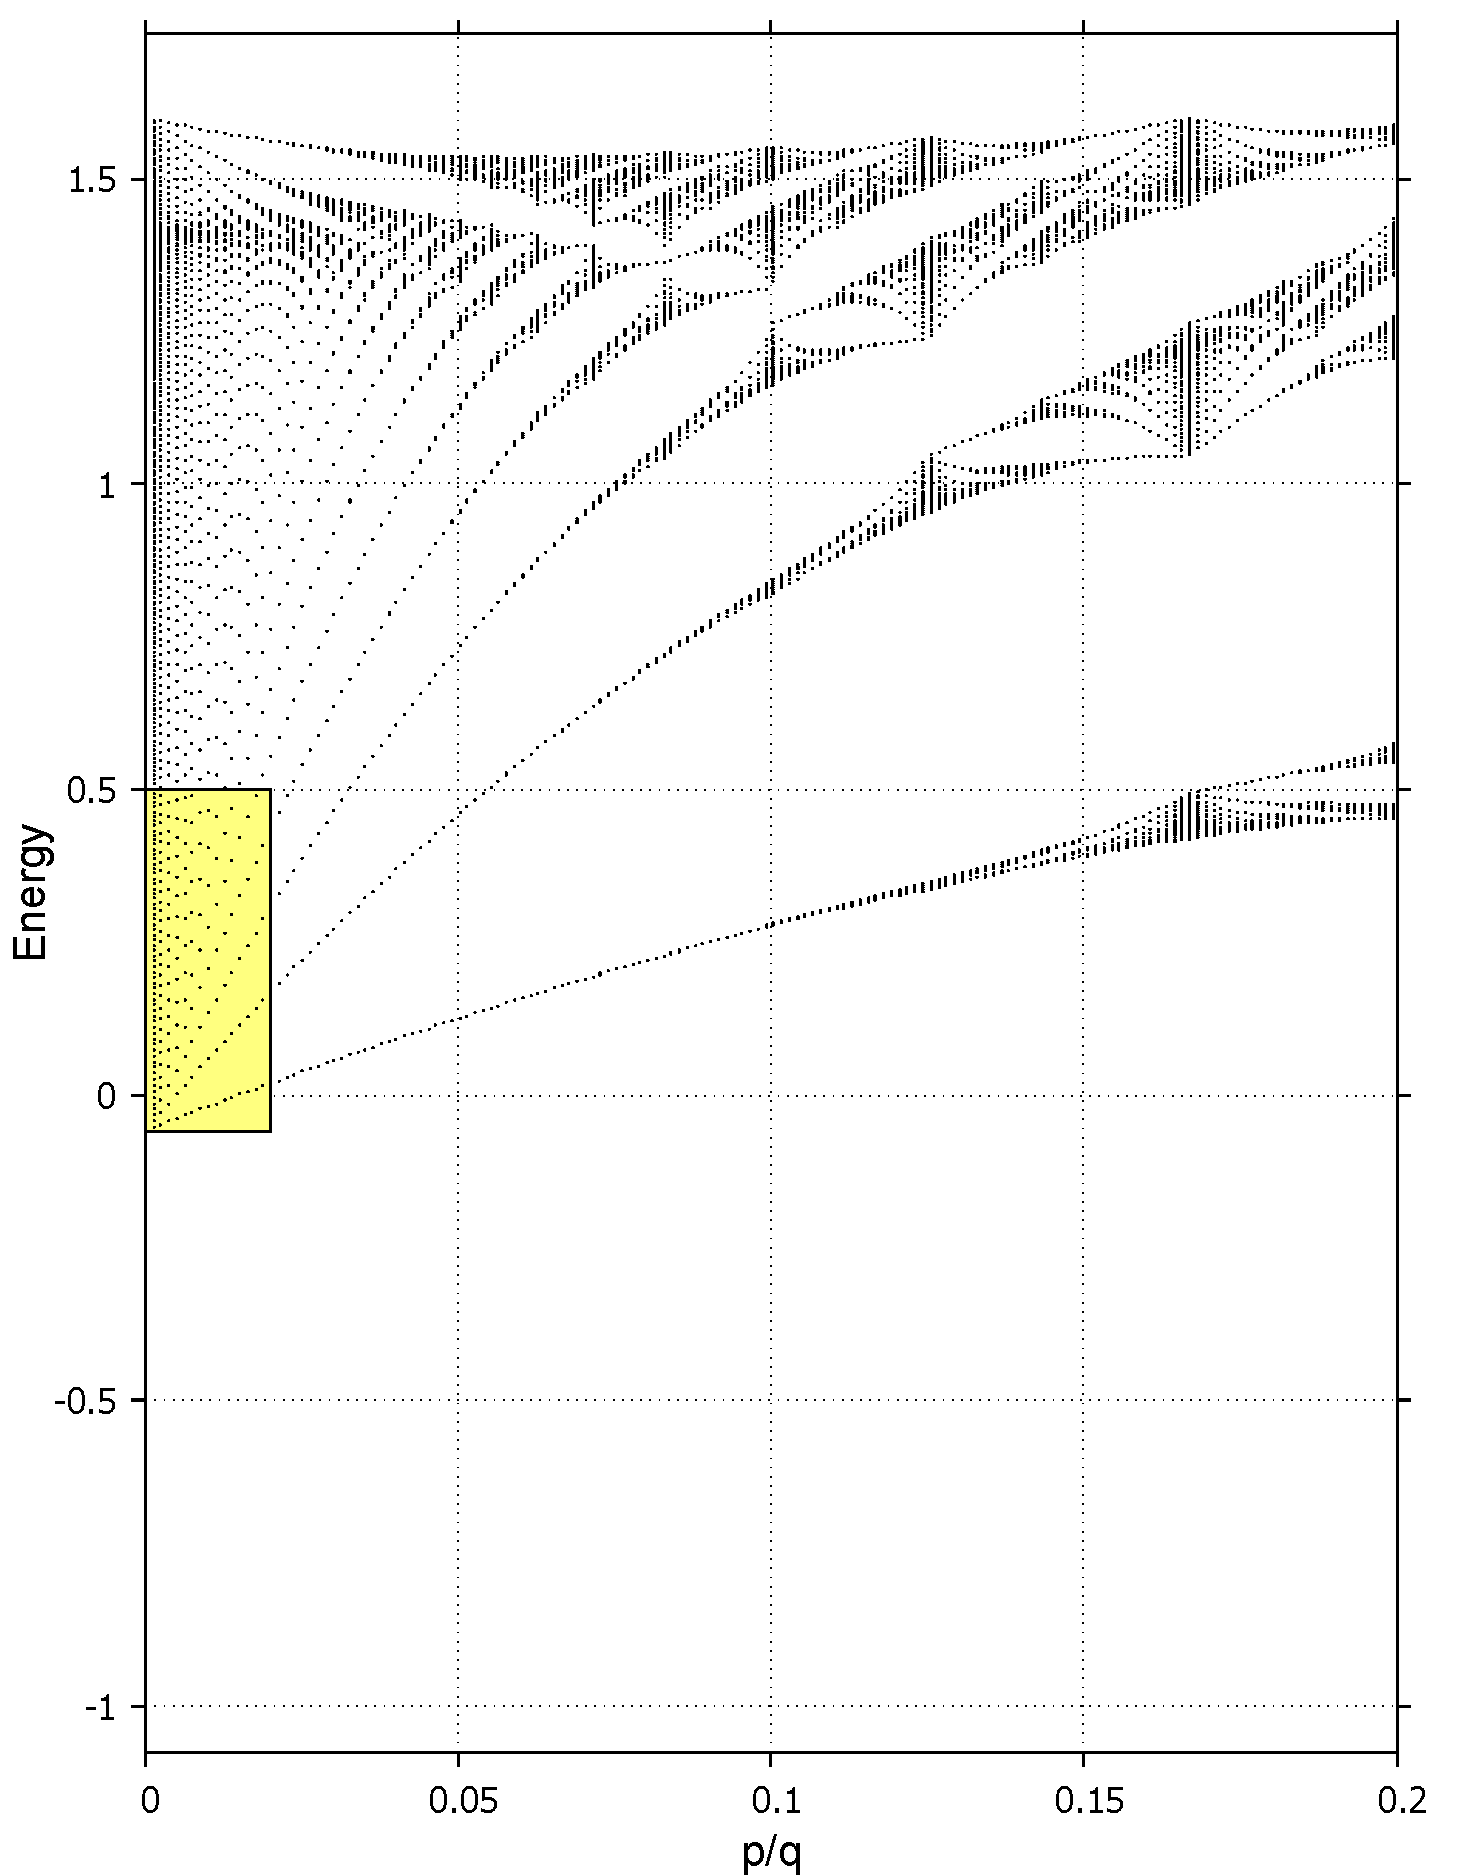
\includegraphics[width=0.85\textwidth,height=1.2\linewidth]{pic/small_area_LL.png}}
	\end{subfigure}
	\begin{subfigure}[b]{0.49\textwidth}
		\centering
		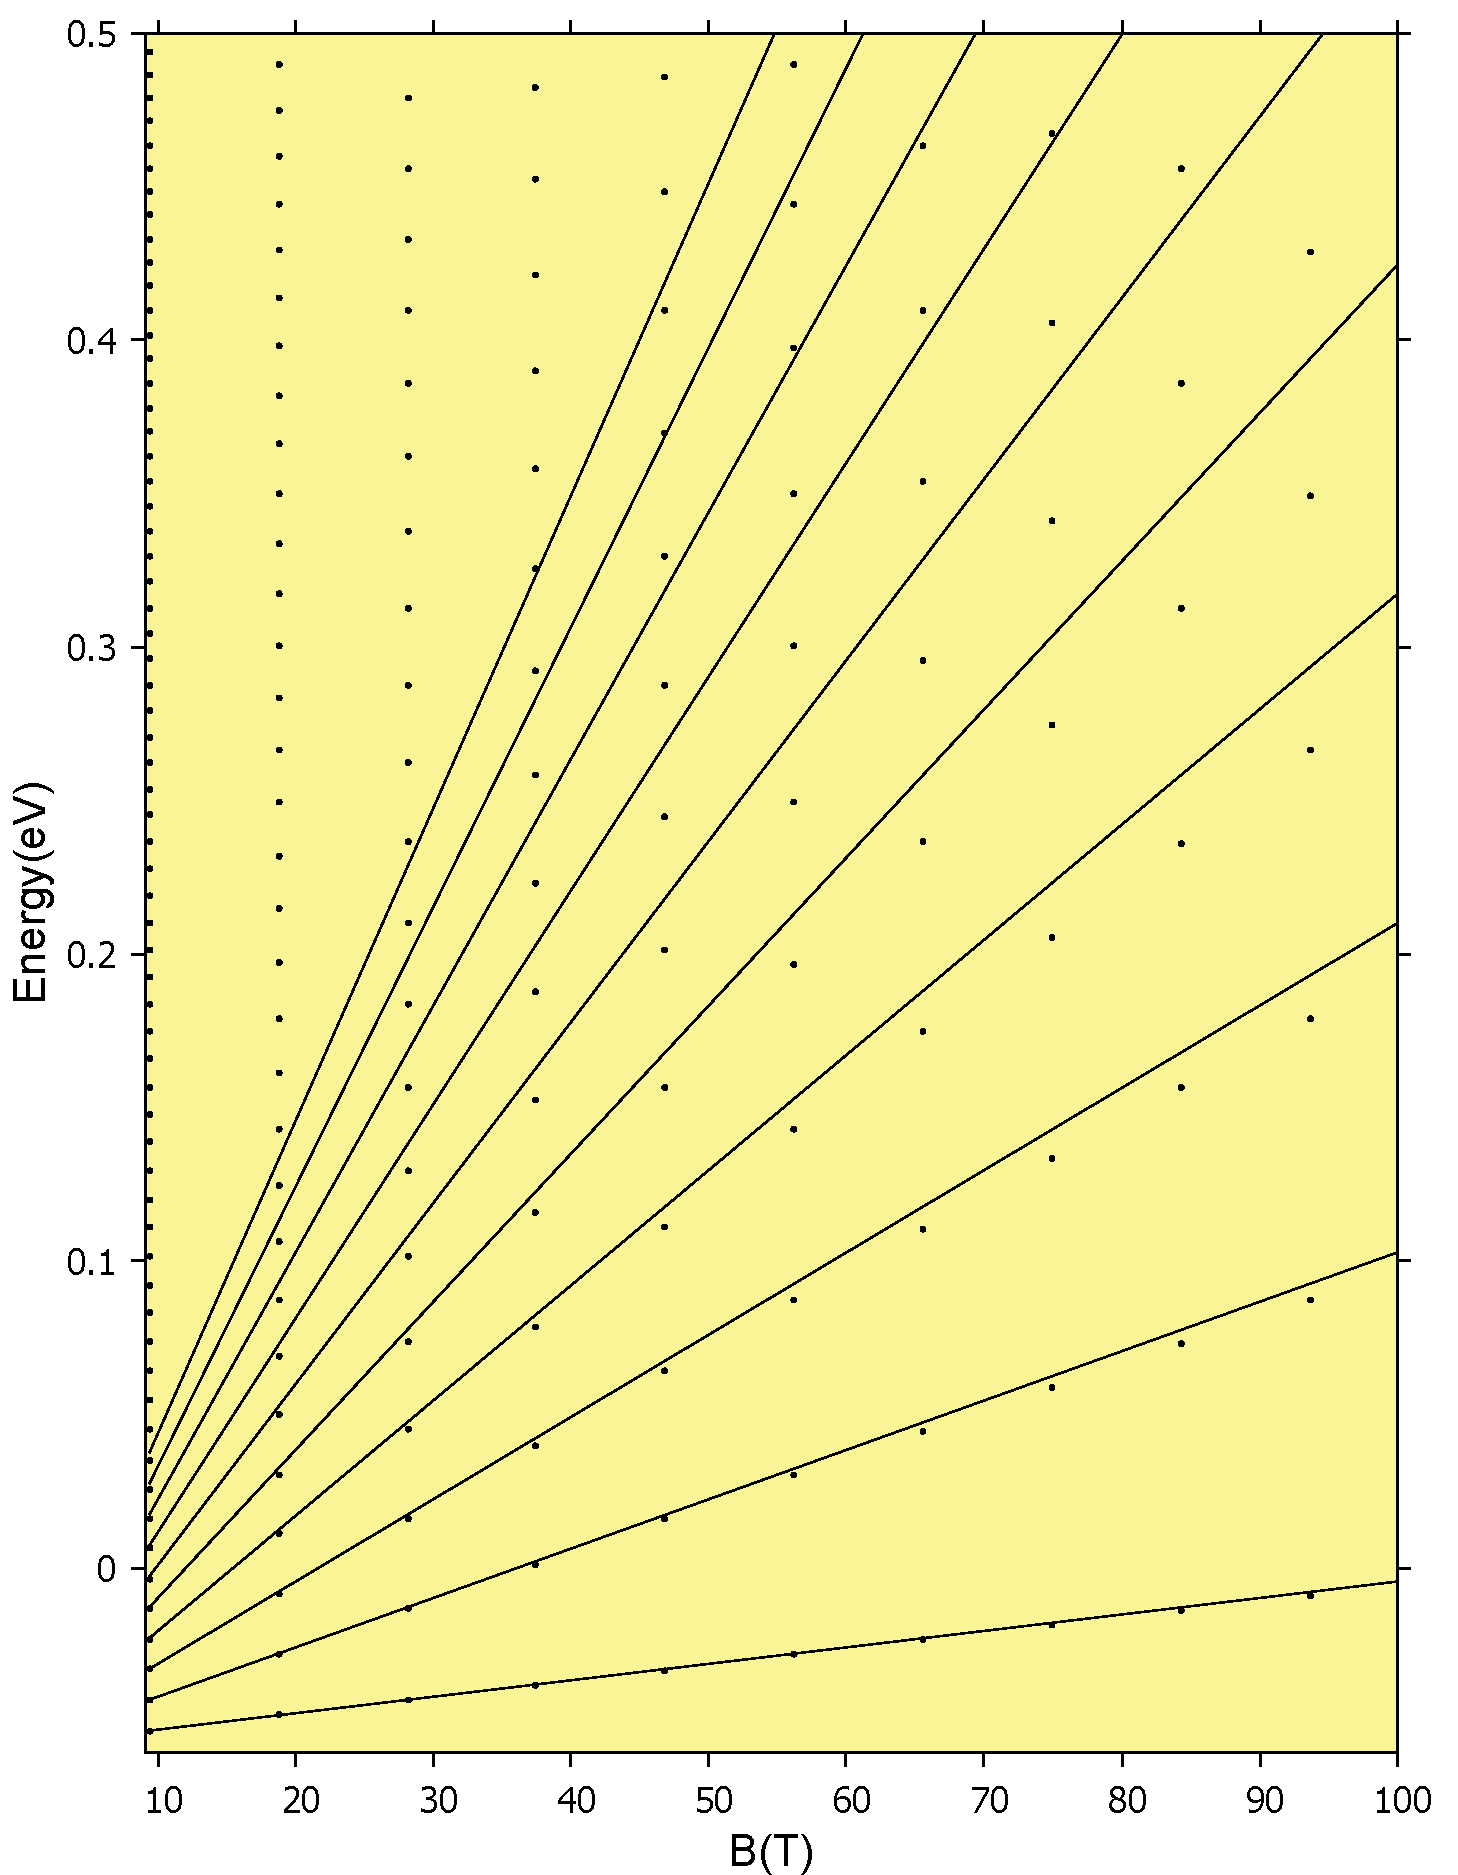
\includegraphics[width=0.85\textwidth,height=1.2\linewidth]{pic/landaulevel_h0_q_797.pdf}
	\end{subfigure}
	\caption[Exploration Landau levels in Hofstadter butterfly.]{
		(a) Same plot as Fig (2.6) but considering a small area and (b) shows superposition of the Landau fan diagram and the Hofstadter butterfly. Display the first $n = 30$ levels near the bottom of the conduction band for a magnetic field up to $B = 500$ T.
	}
\end{figure*}

In Fig 2.9 we compare the spectrum of a small section of single-band with $p / q = 1 / 797$, which is equivalent to small magnetic field, the spectrum of MoS$_{2}$, with the energy of Landau levels given by Eq.(2.50) show standard equally spaced \ac{LLs} \cite{Shoenberg_1984,singleton2001band,blundell2001magnetism,kittel1987quantum} near the bottom of the bands, as plotted in Fig 2.9(b). The fan of \ac{LLs} can be clearly seen emergin from the partern in Fig 2.9(a).

In Fig 2.9(a), there is just single-band in case zero field, with the effective mass $m^{*} = \frac{\hbar}{3 t_{0} a^{2}}$. The numerical result for this portion of the spectrum are shown in Fig 2.9 for $p/q \geq 1/797$. The first few LLs are clearly seen, and the asymtotic slopes $p/q$ at large $q$ given by Eq. (2.50) are shown for comparison for the first five Landau levels at $B \leq 100$ T. At the values of $B$ the fit is not ideal, but it does seem to be improving with the decreasing $p/q$.

Figure 2.9 displays a blowup of the low uniform magnetic region and the \ac{LLs} as a function of $\Phi / \Phi_{0}$ \cite{Li_2011}. The Landau levels are all close to being linear in $B$, resulting from the magnetic quantization of parabolic bands at $B = 0$ T i.e. increasing values of B, these \ac{LLs} are sequentially depleted; for $B=200$ T the levels are completely filled up to the level $n=4$; for $B = 500$ T it happens the same, only this time are filled up to the level $n=1$ and so on.

%More interesting is the top and bottom of conduction and valence band of the zero field spectrum. This results in a non-standard Landau levels when the field is turned on, as discused above.\\
%In the one-band case, knowing the effective mass in zero field and the charge is enough to determine the Landau level spectruc to linear order in the magnetic field. For the three-band case
%
%
% In order to determine the cyclotron frequency for the three-band, through the derivation in Appendix C, we have obtained the Landau levels for the three-band model when the field is turned on
%\begin{figure*}[htb]
%	\centering
%	\begin{subfigure}[b]{0.49\textwidth}
%		\centering
%		{\includegraphics[width=0.85\textwidth,height=1.2\linewidth]{pic/small_area_LL_3band.png}}
%	\end{subfigure}
%	\begin{subfigure}[b]{0.49\textwidth}
%		\centering
%		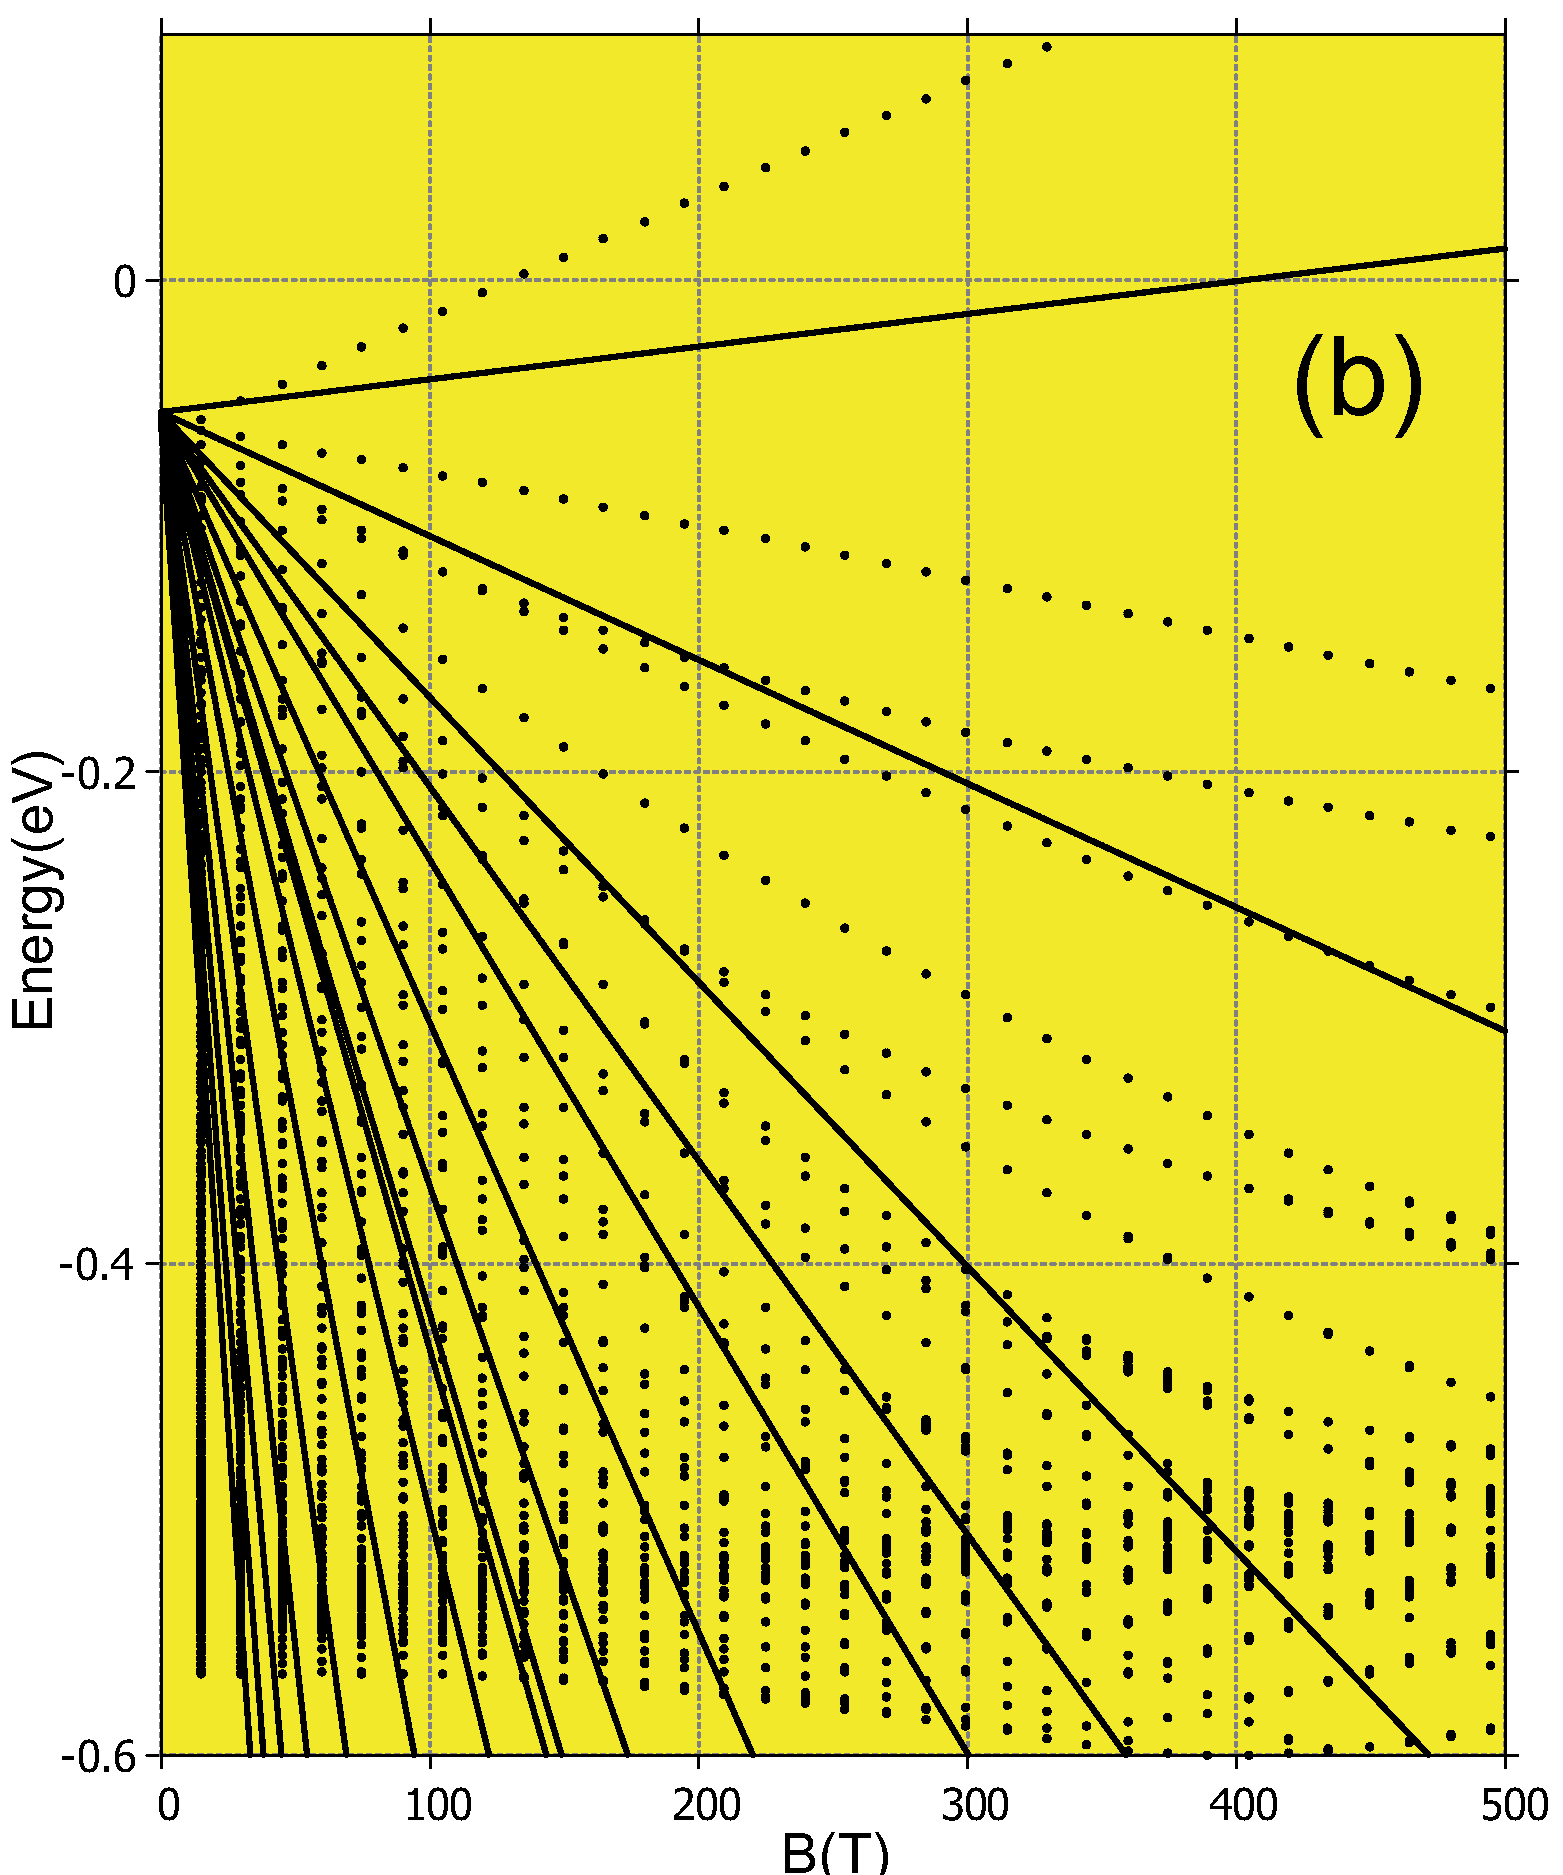
\includegraphics[width=0.85\textwidth,height=1.2\linewidth]{pic/landaulevel_3band_q_797_EF_final.pdf}
%	\end{subfigure}
%	\caption{
%		test
%	}
%\end{figure*}
%Ta có thể thấy một số mức Landau có năng lượng là được tăng tuyến tính theo cường độ từ trường, nhưng lại không cách đều và chính xác như hình của Hofstadter butterfly. Thêm vào đó có nhiều trạng thái mà năng lượng tại đó thì giảm trong khi đó thì từ trường lại tăng. những trạng thái này sẽ được gọi là những trạng thái ``kì cục'' mà ta sẽ bàn luận ở đây.\\
%Trong trường hợp một band, khối lượng hiệu dụng $m^{*}$ và điện tích là đủ để mô tả được phổ Landau theo sự thay đổi tuyến tính của từ trường. Trong trường hợp 2 band và 3 band thì


%It is this fan of Landau levels that responsible for the de Haas-van Alphen and Shubnikov-de Haas effects.

\section{Hall effects}
\subsection{The classical Hall effect}
The Hall effect arises when a conductor carrying an electric current is placed in an external magnetic field $\mathbf{B}$. The Lorentz forece from the magnetic field causes the charges to accumulate on one side of the conductor. Starting with an electric field $\mathbf{E}$ established in the solid results in a current density $\mathbf{J}$ linearly related to the field through Ohm's law
\begin{gather}
	\mathbf{J} = \boldsymbol{\sigma} \mathbf{E}, \\
	\mathbf{E} = \sigma^{-1} \mathbf{J} = \rho \mathbf{J},
\end{gather}
where $\boldsymbol{\sigma}$ is the conductivity tensor and the resistivity $\mathbf{\rho}$ is defined as the inverse of the conductivity. This remains true when both are tensors
\begin{gather}
	\begin{pNiceMatrix}
		J_{x} \\
		J_{y}
	\end{pNiceMatrix}
	=
	\begin{pNiceMatrix}
		\sigma_{xx} & \sigma_{xy} \\
		\sigma_{yx} & \sigma_{yy} \\
	\end{pNiceMatrix}
	\begin{pNiceMatrix}
		E_{x} \\
		E_{y}
	\end{pNiceMatrix}, \\
	\begin{pNiceMatrix}
		E_{x} \\
		E_{y}
	\end{pNiceMatrix}
%	=
	\begin{pNiceMatrix}
		\rho_{xx} & \rho_{xy} \\
		\rho_{yx} & \rho_{yy} \\
	\end{pNiceMatrix}
	\begin{pNiceMatrix}
		J_{x} \\
		J_{y}
	\end{pNiceMatrix}.
\end{gather}
The off-diagonal components of resistivity tensor is $\rho_{xy} = \rho_{yx} = \tfrac{B}{en}$. Usually we measure the resistance $R$, which differs from the resistivity $\rho$ by geometric factors. However, for $\rho_{xy}$, this thing coincide. To see this, consider a sample of material of length $L$ in the $y$-direction. We drop a voltage $V_{y}$ in the $y$-direction and measure the resulting current $I_{x}$ in the $x$-direction. The transverse resistance is
\begin{gather}
	R_{xy} = \frac{V_{y}}{I_{x}} = \frac{L E_{y}}{L J_{x}} = \frac{E_{y}}{J_{x}} = -\rho_{xy}.
\end{gather}
For a current $I_{x}$ flowing in the $x$-direction, and the corresponded electric field $E_{y}$ in the $y$-direction, the Hall coefficent is defined by
\begin{gather}
	R_{H} = \frac{\rho_{xy}}{B} = \frac{1}{en} .
\end{gather}
showing the Hall resistance is a constant in the classical regime. We see that the Hall coefficent depends only on microscopic information about the material: the charge and density of conduction particles. The Hall coefficent does not depend on the scattering time $\tau$; it remains unaffected by the specific frictional mechanism present in the material.
\begin{figure*}[htb]
	\centering
	\begin{subfigure}[b]{0.495\textwidth}
		\centering
		{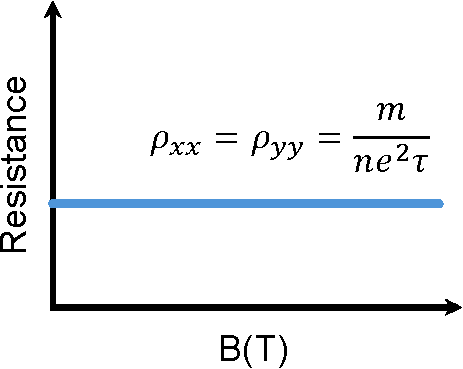
\includegraphics[width=0.75\linewidth]{pic/classRess.pdf}}
	\end{subfigure}
	\begin{subfigure}[b]{0.495\textwidth}
		\centering
		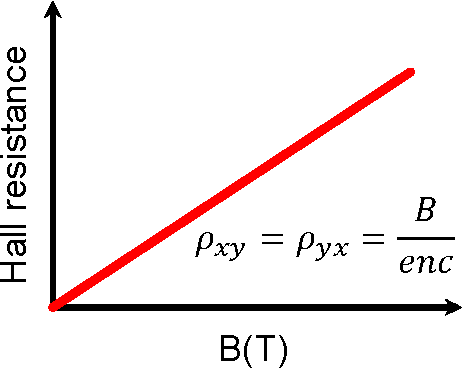
\includegraphics[width=0.75\linewidth]{pic/HallRess.pdf}
	\end{subfigure}
	\caption[Logitudinal resistance and Hall resistance plot.]{
		The longitudinal resistance on the right figure and the Hall resistance in the left figure. The graph shows both the longitudinal resistance and the Hall resistance is linear to the increasing magnetic field.
	}
\end{figure*}
\subsection{The Quantum Hall effect}
In previous section, we arrived at the classical Hall resistance, which remains stable under the classical mechanics framework. However, our world is governed not only by classical physics but also by quantum mechanics. Things changes significantly at extremely low temperatures and strong magnetic fields, revaling new quantum phenomena.

There are two related phenomena which are associated to two different quantum Hall effects. These are called the \ac{IQHE} and \ac{FQHE}. In this study, we mainly focus on the \ac{IQHE} where the flux number and flux quanta are integers. This phenomenon can be understood without taking into account the Coulomb interaction between electrons, which means we will continue using the single electron Hamiltonian that we described in \hyperref[Section 2]{Section 2}. In this section, we first discovered and subsequenly understood theoretically the integer quantum Hall effect in the Hofstadter butterfly.

In two dimensional, there is a crucial relationship between the conductivity tensor $\boldsymbol{\sigma}$ and the resistivity tensor $\boldsymbol{\rho}$ is given by
\begin{equation}
	\begin{aligned}
		\begin{bmatrix}
			\sigma_{xx} & \sigma_{xy} \\
			\sigma_{yx} & \sigma_{yy}
		\end{bmatrix}
		\begin{bmatrix}
			\rho_{xx} & \rho_{xy} \\
			\rho_{yx} & \rho_{yy}
		\end{bmatrix}^{-1}
		=
		\f{1}{\rho_{xx} \rho_{yy} - \rho_{xy} \rho_{yx}}
		\begin{bmatrix}
			\rho_{yy}  & -\rho_{xy} \\
			-\rho_{yx} & \rho_{xx}
		\end{bmatrix}
	\end{aligned}.
\end{equation}
Let's take a look at the experimental data for the quantum Hall effect were perfomed in 1980 by von Klitzing \textit{et at.} \cite{klitzing90}
\begin{figure}[H]
	\centering
	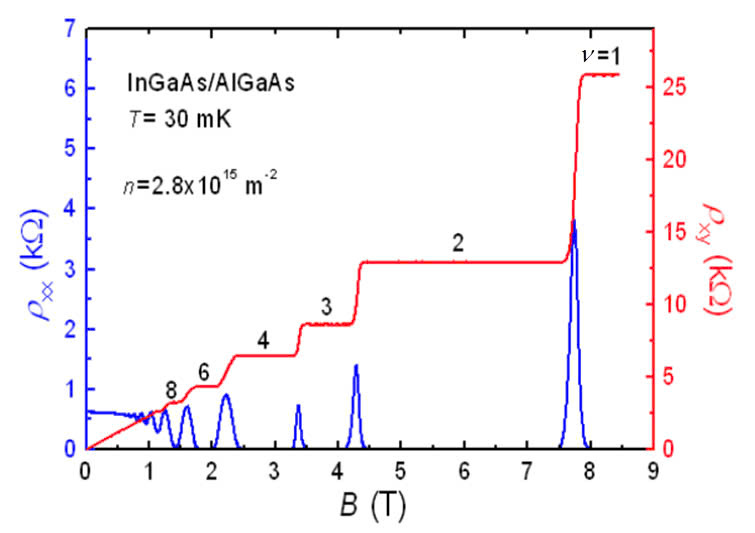
\includegraphics[width=0.7\linewidth]{pic/quantumhall.jpg}
	\caption[Quantum Hall effect by von Klitzing.]{This is the integer quantum Hall effect. For this Klaus von Klitzing was awarded the 1985 Nobel prize.}
\end{figure}
\noindent Both the Hall resistivity $\rho_{xy}$ and the longitudinal resistivity $\rho_{xx}$ depict interesting behaviour. Perhaps the most striking feature in the figure is the fact that the Hall resistivity $\rho_{xy}$ sits on a plateau for a range of magnetic field, before jumping dramatically to the next plateau, while the longitudinal spikes sharply at the transistions between plateuax but vanishes on the plateaux themsleves. \\
The Hall resistivity is now defined
\begin{gather}
	\rho_{xy} = \frac{R_{K}}{\nu}, \quad \nu = 1,2,...
\end{gather}
while $\nu$ is the total filled Landau levels and $R_{K}$ is Klitzing's resistance constant
\begin{gather}
	R_{K} = \frac{h}{e^{2}} = 25812.8074555 \Omega \pm 0.0000059 \Omega.
\end{gather}
Between two plateaux, if $\rho_{xy}  = 0$ then we get the familiar relation between resistivity and conductivity is $\sigma_{xx} = 1/\rho_{xx}$. But on these Hall plateaux
\begin{gather}
	\rho_{xy} = \rho_{yx} = \text{const} ,\; \rho_{xx} = \rho_{yy} = 0 ,
\end{gather}
this leads to
\begin{gather}
	\sigma_{xy} = \sigma_{yx} = 1 / \text{const} , \; \sigma_{xx} = \sigma_{yy} = 0.
\end{gather}
There is an apparent paradox here, we would call a system with $\rho_{xx} = 0$ is a perfect conductor, while one with $\sigma_{xx} = 0$ is a perfect insulator. But what if both $\rho_{xx} = 0$ and $\sigma_{xx} = 0$ occur simultaneously? A new material or a new state of matter?


\subsection{Color the Hofstadter butterfly}
The contribution to the Hall conductivity from a single subband is given by \cite{kohmoto1989,hatsugai1990energy,kohmoto1985topological,thouless1982}
\begin{gather}
	\sigma_{xy} = \f{e^{2}}{h} \sum_{n}^{\text{occ.}} \f{1}{2\pi} \dps\oiint_{\text{{BZ}}} d k_{x} d k_{y} \Omega_{n}^{z} (\mathbf{k}).
\end{gather}
In general, the Berry curvature intergrated over a closed manifold is quantized in the units of $e^{2} / h$ and equals to the net number of monopoles inside. This number is called the Chern number and is responsible for a number of quantization effects. Therefore the Hall conductivity is quantized for a two dimensional band insulator of noninteracting electrons. Since the integral for the whole Brillouin zone respectively Berry curvature, we arrived at the \ac{TKNN}'s formula \cite{thouless1982}
\begin{gather}
	\sigma_{xy} = \f{e^{2}}{h} \nu, \quad \nu = 1,2,...
\end{gather}
$\nu$ is guaranteed to be an integer given by the Chern number.

%With the cyclotron frequency in Section 2.4, the electron energy is quantized to the Landau levels.

We, then, calculate the quantum Hall conductivity by the Streda formula \cite{streda1982}
\begin{gather}
	\sigma_{xy}(B,E_{F}) = e \f{\partial N (E,B)}{\partial B} \at{E=E_{F}}{},
\end{gather}
%As show in Fig. (2.12), the Hall conductivity is quantized at colored points.
where $N(E_{F},B)$ is the number of state at fixed Fermi energy $E_{F}$. Combining Eq. (2.66) and Eq. (2.67), we have
\begin{gather}
	\f{\partial N}{\partial B} = \f{e}{h} \nu.
\end{gather}
Assuming that $B$ vary slightly
\begin{gather}
	N = c + \f{e}{h}B \nu, \quad c \; \text{is any constant}.
\end{gather}
Before this, we have defined $\frac{p}{q} = \frac{eBa^{2}\sqrt{3}}{4h}$, with $S = \frac{\sqrt{3} a^{2}}{4}$ is the area of the original unit cell in \hyperref[Section 2.2]{Section 2.2}. Multiply $S$ with Eq. (2.69), we have
\begin{gather}
	N \times S = c + \f{p}{q} \nu,
\end{gather}
and the density of electron in a single band is given by $\frac{1}{Sq}$, thus when there are $r$ bands below the Fermi energy level, the density of electron for $r^{\text{th}}$ band is
\begin{gather}
	N = \f{r}{Sq}.
\end{gather}
Then, the Eq. (2.70), is written as,
\begin{gather}
	r = c \times q + p \times \nu_{r},
\end{gather}
in this equation $r$, $q$, $p$, $\nu$ are integers, thus, $c\times q$ must be an integer. On the one hand, since $c$ is independent of $q$, and $q$ can change when the magnetic field is varied without making a point of contact, then $c$ itself must be an integer, namely $s_{r}$. Thus we have
\begin{gather}
	r = q \times s_{r} + p \times \nu_{r},
\end{gather}
this equation is usually named as the Diophantine equation. While $\nu$ is the Chern number associated with the quantized Hall conductance, $s$ is another integer that play a role to indentify the gap index.

The Hall conductivity of the lattice model for an electron in a background magnetic field can only be computed when the flux ratio $\frac{\Phi}{\Phi_{0}} = \frac{p}{q}$ is rational. In this case, we can use the TKNN formula, but with the Chern number, which used to be defined by intergrating over the Brillouin zone, now arising by intergrating over the magnetic Brillouin zone. Others derivation is in \cite{di2022linking,dana1985,avron2003}.

The Diophantine equation is crucial in understanding the quantization of Hall conductance in the Hofstadter butterfly. The Chern number $\nu$ determines the topological nature of the bands and their contribution to the Hall conductance, while the integer $s$ identifies specific energy gaps in the spectrum. These gaps are directly linked to incompressible quantum Hall states, which are of significant interest in both theoretical and experimental condensed matter physics.

To further explore the intricate fractal nature of the Hofstadter spectrum, we shall now achieve the colored Hofstadter butterfly. There are many ways to color the butterfly. For instance, a common approach is to color each point of the butterfly based on their Chern number, as illustrated in the Fig 2.12. At these points, the Hall conductivity hightlights exactly quantization. However, a drawback of this method is that the butterfly may contain a dense of points, which can make it difficult to visualise fine details in the colored spectrum. 
\begin{figure*}[htb]
	\centering
	\begin{subfigure}[b]{0.495\textwidth}
		\centering
		{\includegraphics[width=\linewidth]{pic/1band_Chern_q_199_test.png}}
	\end{subfigure}
	\begin{subfigure}[b]{0.495\textwidth}
		\centering
		\includegraphics[width=\linewidth]{pic/3band_Chern_q_199_test.png}
	\end{subfigure}
	\caption{
		q = 199 và q = 797
	}
\end{figure*}
%	\begin{subfigure}[b]{0.495\textwidth}
%	\centering
%	\includegraphics[width=0.85\textwidth,height=1.2\linewidth]{pic/wannier_gnu.pdf}
%\end{subfigure}



\begin{figure*}[htb]
	\centering
	\begin{subfigure}[b]{0.495\textwidth}
		\centering
		\includegraphics[width=\linewidth]{pic/1band_Chern_q_797_colorplane2.png}
	\end{subfigure}
	\begin{subfigure}[b]{0.495\textwidth}
		\centering
		\includegraphics[width=\linewidth]{pic/3band_Chern_q_797_colorplane2.png}
	\end{subfigure}
	\caption[Colorplaned Hofstadter butterfly.]{
		q = 199 và q = 797. This color pallete was famously made by Avron\cite{avron2003}.
	}
\end{figure*}
\begin{figure*}[htb]
	\centering
	\begin{subfigure}[b]{0.495\textwidth}
		\centering
		\includegraphics[width=\linewidth]{pic/1band_Chern_q_797_colorplane.png}
	\end{subfigure}
	\begin{subfigure}[b]{0.495\textwidth}
		\centering
		\includegraphics[width=\linewidth]{pic/3band_Chern_q_797_colorplane.png}
	\end{subfigure}
	\caption[Colorplaned Hofstadter butterfly.]{
		q = 199 và q = 797. This color pallete was famously made by gnuplot.
	}
\end{figure*}


Fig 2.13 displays the Hofstadter butterfly, color-coded according to the Hall conductance. Moreover, the number $p$ increases simultaneously with Chern number, making it challenging to maintain a fixed scale. Therefore, to address this, we limit the Chern number scale within $-10 \leq \nu \leq 10$, any Chern number outside this range is set to zero. Regions with zero Hall conductance and the corresponding spectrum are left blank. Remarkably, the two largest gaps near the center of the figure are associated with small integers where the color coding accurately reflects their values. Unlike the traditional Hofstadter butterfly, which hightlights the spectrum, this version emphasizes the gaps by using a color scheme to characterize different Hall conductance.

\newpage

Both figures display rich physics insights, it totally use two different methods to color the butterfly. While Figure 2.12 uses the sum of the Chern numbers of the occupied bands, Figure 2.13 relies only on the Chern numbers that corresponded to the gap index. However, the colored spectrum not only helps visualize the topological properies of the sysem but also both explain that as the magnitude $B$ increases, the number of occupied bands decreases.


%\subsection{Wannier diagram}
% a simplified replica of Fig, a powerful tool for visualizing the relationship between magnetic flux and electron filling in the system. Wannier's diagram provides a graphical representation of the allowed energy gaps in the Hofstadter spectruc as a function of the magnetic flux per unit cell and the electron filling factor. This diagram is particularly insightful because it captures the topological properties of the system through the distribution and behavior of these energy gaps.
%
%The fundamental of Wannier's diagram lies in the Diophantine gap equation
%\begin{gather}
%	\f{n}{n_{0}} = \nu \f{\Phi}{\Phi_{0}} + s,
%\end{gather}
%where $\frac{n}{n_{0}}$ is the electron filling factor, representing the ratio of the number of electrons per unit cell, $\nu$ is the Chern number associated with the quantized Hall conductance, and $s$ is another interg that corresponds to the gap index, effectively indicating the electron filling within the spectrum.
%
%
%
%The calculated Wannier's diagram, the energy density of state as a function of filling factor $\frac{n}{n_{0}}$ and magnetic flux $\Phi$ as illustrated in Fig, reveal the presence of these energy gaps across the spectrum. Each colored line in the diagram corresponds to an energy gap where the system exhibits an imcompressible quantumm Hall state, characterized by a quantized Hall conductance. The diagram not only provides a clear visualization of the gap structure but also offers insights into the topological phases that arise in monolayer TMD systems under varying magnetic flux conditions.
%\begin{figure}[H]
%	\centering
%	\includegraphics[width=0.8\textwidth,height=0.85\linewidth]{pic/wannier199.png}
%	\caption{Wannier diagram}
%\end{figure}

\chapter{RESULT AND DISCUSSION}
\chapter{CONCLUSION AND FUTURE WORK}
\section{Conclusion}
In our research, we have calculated the Hofstadter butterfly of monolayer MoS$_{2}$ and others transistion metal dichalcogenide types by using a tight-binding three-band model. In addition, we have explored the rich and complex physics of monolayer MoS$_2$, such as Landau levels and integer quantum Hall effect (IQHE), in the presence of external magnetic fields. The research conducted within these pages has demonstated the unique interplay between the superlattice and magnetic fields, which leads to the emergence of fascinating quantum phenomena. 

In section 2.1, we have studied the tight-binding three-band model for monolayers of MX$_{2}$ using only the M$-d_{z^{2}}$, $d_{xy}$ and $d_{x^{2} - y{^2}}$ orbitals. When only NN M-M hoppings are included, we calculated the hopping energies using the symmetry of the $D_{3h}$ point group we derived eights hopping parameters from Ref \cite{PhysRevB.88.085433}.

In section 2.2, we focused on the Hofstadter physics in monolayer TMD, where the lattice gives rise to a rich Hofstadter spectrum when subjected to a magnetic field. The detailed analysis revealed key features of the spectrum, including the SOC and the emergence of topological quantum Hall states. In addition, the study also demonstrated that there are many ways to derivive the Hofstadter spectrum two of those is using the Peierls substitution or Envelope Function Approximation.

In section 2.3 and section 2.4, extended the investigation into the realm of Hall effects, introducing the Landau levels, the integer quantum Hall effect and applying it to monolayer TMD systems. We also shown that how the Hofstadter butterfly can be colored in various ways using the Chern number.

Overall, while this study provides valuable insights, we acknowledge several limitations. Firstly, in section 2.3, our calculation was restrited to the single-band approximation due to the computational complexity of multi-band interactions. Specifically, incorporating three-band model would require significantly more resources, particularly in calculating Chern numbers, which are numerically intensive for larger Hamiltonian matrices, this significantly cause a time consumption. For example, to achived the colored butterfly, it costs us around two days for a better resolution.
\section{Future work}
For further research, we 




\appendix
\renewcommand{\chaptername}{Appendix}
%\chaptermark{Appendix}
%\begin{appendices}
%	\section{1}
%\end{appendices}

\chapter{Details of the Peierls substitution} \label{appendix a}
As we mentioned in Section 2.2, we work in the Landau gauge $\mathbf{A} = (0,Bx,0)$. The Peierls phase is given as $\theta_{i,i'} = \int_{i}^{i'}\mathbf{A} \cdot d\mathbf{r}$. By making an parametrization, for instance
\begin{gather}
	\begin{cases}
		x = x_{m} + (x_{m'} - x_{m}) \tau, \\
		y = y_{n} + (y_{n'} - y_{n}) \tau,
	\end{cases}
\end{gather}
where $\tau \in \left[0,1\right]$ and $i = (m,n)$, thanks to the Landau gauge, the path integral resembles to $\int Bx dy$, the phases can be written as
\begin{equation}
	\begin{aligned}
		\theta_{i,i'} &= \frac{eB}{\hbar} \int_{0}^{1} \left[ x_{m} + (x_{m'} - x_{m}) \tau \right] (y_{n'} - y_{n}) d\tau \\
		&= \frac{eB}{\hbar}(x_{m} + \frac{x_{m'} - x_{m}}{2})(y_{n'} - y_{n}) \\
		&= \frac{eB}{\hbar}\left(\frac{x_{m} + x_{m'}}{2}\right)(y_{n'} - y_{n}).
	\end{aligned}
\end{equation}
From this, the Peierls phase depends on absolute $x$ coordinates but only relative to $y$ coordinates.

\chapter{Harper's equation} \label{appendix b}
%We now consider the Harper equation fo the case where the crystal lattice is a square lattice, given by the Hamiltonian from the example in the text \cite{yalcin_2019}
%\begin{equation}
%	\begin{aligned}
%		H(\mathbf{k})
%		 & = 2 t \left[\cos(k_{x} a) + \cos(k_{y} a)\right]                               \\
%		 & = t \left[ e^{ik_{x} a} + e^{-ik_{x} a} + e^{ik_{y} a} + e^{-ik_{y} a} \right]
%	\end{aligned}
%\end{equation}
%By using Peierls's substitution $\hbar\mathbf{k} \rightarrow (\mathbf{\Pi} - e \mathbf{A})$, ta có
%\begin{equation}
%	\begin{aligned}
%		H & = t \left[ e^{ik_{x} a} + e^{-ik_{x} a} + e^{i (p_{y} - e Bx) a/\hbar} + e^{-i (p_{y} - e Bx) a/\hbar} \right]                                    \\
%		  & = t \left[ e^{ik_{x} a} + e^{-ik_{x} a} + e^{i p_{y} a/\hbar} e^{i 2 \pi Bx / \Phi_{0}} + e^{-i p_{y} a/\hbar} e^{-i 2 \pi Bx / \Phi_{0}} \right]
%	\end{aligned}
%\end{equation}
%Substituting $x = ma$ and $y = na$ given the coordinates of the square lattice, we obtain the Harper equation
%
We now consider the case of hexagonal lattice with one band as a basis under an uniform magnetic field given by the Landau gauge $\mathbf{A} = (0, Bx,0)$. Given

\begin{equation}
	\begin{aligned}
		h_0
		 & = 2 t_0 \left(\cos2\alpha + 2\cos\alpha \cos\beta\right) + \epsilon_1                                                                                                                                     \\
		 & = 2t_{0} \left[ \cos(k_x a) + 2 \cos \left(\f{k_x a}{2}\right) \cos \left(\f{\sqrt{3}k_y a}{2}\right) \right] + \epsilon_1                                                                                \\
		 & = 2t_{0} \left\{ \cos(k_x a) + \cos\left[\left( k_{x} + \sqrt{3} k_{y} \right)\frac{a}{2}\right] + \cos\left[\left( k_{x} - \sqrt{3} k_{y} \right)\frac{a}{2}\right]\right\} + \epsilon_1                 \\
		 & = 2t_{0} \Biggl\{ \cos(\Pi_{x}\f{a}{\hbar}) + \cos \left[\left(\Pi_{x} + \sqrt{3} e B x + \sqrt{3} \Pi_{y}\right)\frac{a}{2\hbar}\right]                                                                  \\
		 & + \cos \left[\left(\Pi_{x} - \sqrt{3} e B x - \sqrt{3} \Pi_{y}\right)\frac{a}{2\hbar}\right] \Biggr\} + \epsilon_1                                                                                        \\
		 & = t_{0} \biggl[e^{i \Pi_{x}\frac{a}{\hbar}} + e^{-i\Pi_{x}\frac{a}{\hbar}} + e^{i(\Pi_{x} + \sqrt{3} eBx + \sqrt{3} \Pi_{y} ) a / 2\hbar} + e^{-i(\Pi_{x} + \sqrt{3} eBx + \sqrt{3} \Pi_{y} ) a / 2\hbar} \\
		 & + e^{i(\Pi_{x} - \sqrt{3} eBx - \sqrt{3} \Pi_{y} ) a / 2\hbar} + e^{-i(\Pi_{x} - \sqrt{3} eBx - \sqrt{3} \Pi_{y} ) a / 2\hbar} \biggr] + \epsilon_1.
	\end{aligned}
\end{equation}
We replaced $\hbar \mathbf{k}$ in the above function by the operators $\mathbf{\Pi} + e \mathbf{A} / c$ in order to create an operator out of $h_{0}$. However, the quantity $\hbar \mathbf{k}$ is represents the crystal momentum, it is more precise interpretation is to regard $\mathbf{k}$ as a quantum number which describes a Bloch state. This method can be achived by using \ac{EFA}. However, we must be very careful regarding how the operators act on the wave functions, since $\left[x,\Pi_{x}\right] \neq 0$. In their article, Gumbs and Fekete \cite{gumps1997}  incorrectly applied the modified translation operators, leading to completely incorrect results. In this work, we treat the operators more correctly by applying the \ac{BCH} formula and taking into account the commutation relation $\left[x,\Pi_{x}\right] = i \hbar$
\begin{equation}
	\begin{aligned}
		e^{\pm i(\Pi_{x} + \sqrt{3} e B x) a / 2\hbar}
		 & = e^{\pm i \Pi_{x} a / 2 \hbar} e^{\pm i\sqrt{3} e B x a / 2 \hbar} e^{-\frac{1}{2} \left[\pm i \Pi_{x}, \pm i \sqrt{3} e B x\right] a^{2} / 2 \hbar^{2}} \\
		 & = e^{\pm i \Pi_{x} a / 2 \hbar} e^{\pm i\sqrt{3} e B x a / 2 \hbar} e^{\mp i \sqrt{3} e B a^{2} / 8 \hbar}.
	\end{aligned}
\end{equation}
Substituting $x = \f{ma}{2}$ into (B.2), this leads to
\begin{gather}
	e^{\pm i(\Pi_{x} + \sqrt{3} e B x) a / 2\hbar}
	= e^{\pm i \Pi_{x} a / 2 \hbar} e^{\pm i\sqrt{3} e B (m + 1 /2) a^{2} / 4 \hbar}.
\end{gather}
And
\begin{equation}
	\begin{aligned}
		e^{\pm i(\Pi_{x} - \sqrt{3} e B x) a / 2\hbar}
		 & = e^{\pm i \Pi_{x} a / 2 \hbar} e^{\mp i\sqrt{3} e B x a / 2 \hbar} e^{-\frac{1}{2} \left[\pm i \Pi_{x}, \mp i \sqrt{3} e B x\right] a^{2} / 2 \hbar^{2}} \\
		 & = e^{\pm i \Pi_{x} a / 2 \hbar} e^{\mp i\sqrt{3} e B x a / 2 \hbar} e^{\mp i \sqrt{3} e B a^{2} / 8 \hbar},
	\end{aligned}
\end{equation}
substituting $x = \f{ma}{2}$ into (B.4), this leads to
\begin{gather}
	e^{\pm i(\Pi_{x} - \sqrt{3} e B x) a / 2\hbar}
	= e^{\pm i \Pi_{x} a / 2 \hbar} e^{\mp i\sqrt{3} e B (m - 1 /2) a^{2} / 4 \hbar}.
\end{gather}
The operators $e^{\pm i \Pi_{x} a / 2 \hbar}, e^{\pm i \Pi_{y} \sqrt{3}a / 2 \hbar}$ can be regconized as translational operators, we can rewrite (B.3) as
%The time-indepentdent Schr\"{o}dinger's equation now becomes
\begin{equation}
	\begin{aligned}
		  & t_{0} \varphi_{0} (x + a,y) + t_{0}\varphi_{0} (x - a,y) + t_{0}\varphi_{0} (x + \frac{a}{2},y + \frac{a\sqrt{3}}{2}) e^{\frac{ie}{\hbar}B(m + 1 /2) \frac{a^{2}\sqrt{3}}{4}}                                                            \\
		+ & t_{0} \varphi_{0} (x + \frac{a}{2},y - \frac{a\sqrt{3}}{2}) e^{-\frac{ie}{\hbar}B(m + 1/2) \frac{a^{2}\sqrt{3}}{4}} + t_{0} \varphi_{0} (x - \frac{a}{2},y + \frac{a\sqrt{3}}{2}) e^{\frac{ie}{\hbar}B(m + 1/2) \frac{a^{2}\sqrt{3}}{4}} \\
		+ & t_{0} \varphi_{0} (x - \frac{a}{2},y - \frac{a\sqrt{3}}{2}) e^{-\frac{ie}{\hbar}B(m - 1/2) \frac{a^{2}\sqrt{3}}{4}} + \epsilon_{1} \varphi_{0}(x,y) = E_{1} \varphi_{0}(x,y),
	\end{aligned}
\end{equation}
for the sake of simplicity we have defined $\varphi_{0} \equiv \ket{d_{z^{2}}}$.\\
%We have established in Section 2.2 that when translated by a lattice vector $\mathbf{R}$, the wavefuntion for an electron in a periodic lattice picks up a phase correspondingly. This lets us define
%\begin{gather}
%	\varphi(x \pm a,y) = e^{\pm i k_{x} a} \varphi(x,y), \\ 
%	\varphi(x \pm \f{a}{2},y \pm \f{a\sqrt{3}}{2}) = e^{\pm i k_{x} \frac{a}{2}} e^{\pm i k_{y} \frac{a\sqrt{3}}{2}} \varphi(x,y).
%\end{gather}
%Substituting $x = m \f{a}{2}$ and $y = n \f{a\sqrt{3}}{2}$ for the given hexagonal lattice, we can express the time-indepentdent Schr\"{o}dinger equation as 
%\begin{equation}
%	\begin{aligned}
%		&t_{0} \varphi_{0}(m + 2, n) + t_{0} \varphi_{0}(m - 2, n) + t_{0} \varphi_{0}(m + 1, n + 1) e^{\frac{ie}{\hbar}Bm \frac{a^{2}\sqrt{3}}{4}} \\
%		+& t_{0} \varphi_{0}(m + 1, n - 1) e^{-\frac{ie}{\hbar}Bm \frac{a^{2}\sqrt{3}}{4}} + t_{0} \varphi_{0}(m - 1, n + 1) e^{\frac{ie}{\hbar}Bm \frac{a^{2}\sqrt{3}}{4}} \\
%		+& t_{0} \varphi_{0}(m - 1, n - 1) e^{-\frac{ie}{\hbar}Bm \frac{a^{2}\sqrt{3}}{4}} + \epsilon_{1} \varphi_{0}(m,n) = E_{1} \varphi_{0}(m,n).
%	\end{aligned}
%\end{equation}
It is reasonable to assume planewave behavior in the $y$ direction, since the coefficents in the above equation only involve $x$. Therefore, we can assume the partial solution for $y$ to be in the form
\begin{gather}
	\varphi(\frac{ma}{2},\frac{na\sqrt{3}}{2}) = e^{i k_{y} n \frac{a\sqrt{3}}{2}} \varphi(m),
\end{gather}
which reduces (B.6) to
\begin{equation}
	\begin{aligned}
		  & t_{0} \varphi_{0}(m + 2) + t_{0} \varphi_{0}(m - 2) + t_{0} \varphi_{0}(m + 1) e^{2 i \pi (m + 1 /2) p/ q} e^{i k_{y} a\sqrt{3} / 2}                              \\
		+ & t_{0} \varphi_{0}(m + 1) e^{-2 i \pi (m + 1 /2) p/ q} e^{-i k_{y} a\sqrt{3} / 2} + t_{0} \varphi_{0}(m - 1) e^{2 i \pi (m - 1 /2) p/ q} e^{i k_{y} a\sqrt{3} / 2} \\
		+ & t_{0} \varphi_{0}(m - 1) e^{-2 i \pi (m - 1 /2) p/ q} e^{-i k_{y} a\sqrt{3} / 2} + \epsilon_{1} \varphi_{0}(m) = E_{1} \varphi_{0}(m),
	\end{aligned}
\end{equation}
this is equivalent to Eq. 2.16 we have mentioned in Section 2.2. Equation B.8 is sometimes called ``Harper's equation''\cite{harper1955general,PhysRevB.14.2239} Since different $m$ values give different equations, one reaches a unique set of equations when $\Phi / \Phi_{0}$ is a rational number $p / q$ and $m$ goes through $q$ different values, essentially resulting in the Hamiltonian matrix written for a magnetic unit cell enlarged in $x$ direction $q$ times.\\

In the case of TMD presented in \cite{PhysRevB.88.085433}, the contribution of the
$X$ atom has been neglected, leading to the transformation of the hexagonal crystal structure of TMD into a regular triangular lattice. From there, we can map the triangular lattice to the case of the square lattice. In the triangular lattice, it has been established that the translation operators must satisfy the Baker-Campbell-Hausdorff formula.
\chapter{Solving the Diophantine equation}
We have defined that the magnetic flux through a unit cell is $\frac{\Phi}{\Phi_{0}} = \frac{p}{q}$. For $p$ and $q$ are mutually prime numbers, we defined the pairs $(\nu_{r},s_{r})=(m,n)$ as the solutions for Diophantine equation
\begin{gather}
	p m + q n  = \gcd(p,q).
\end{gather}
Fortunately, $p$ and $q$ are co-prime, (B.1) is now
\begin{gather}
	pm + qn = 1,
\end{gather}
By deviding $p$ by $q$, we get a quotient $a$ and a remainder $b$. They satisfy
\begin{gather}
	q = p a + b.
\end{gather}
By using the Euclidean Algorithm, we can easily find $(m,n)$. For instance, the rational magnetic flux is $\frac{p}{q} = \frac{30}{47}$, then the diophantine equation now is $30m + 47n = 1$, and
\begin{equation}
	\begin{aligned}
		47 = 30 \times 1 + 17, \\
		30 = 17 \times 1 + 13, \\
		17 = 13 \times 1 + 4,  \\
		13 = 4 \times 3 + 1.   \\
	\end{aligned}
\end{equation}
At this point we stop, because we arrived at the greatest common divisor, so the algorithm is over. The next step is solve for the remainders
\begin{equation}
	\begin{aligned}
		47 = 30 \times 1 + 17 \Rightarrow 17 = 47 \times 1 + 30 \times (-1), \\
		30 = 17 \times 1 + 13 \Rightarrow 13 = 30 \times 1 + 17 \times (-1), \\
		17 = 13 \times 1 + 4 \Rightarrow 4 = 17 \times 1 + 13 \times (-1),   \\
		13 = 4 \times 3 + 1 \Rightarrow 1 = 13 \times 1 + 4 \times (-3).
	\end{aligned}
\end{equation}
We are going to take this last remainder equation, and do backwards substitute until we get the very first remainder
\begin{equation}
	\begin{aligned}
		1 & = 13 \times 1 + 4 \times (-3)                              \\
		& = 13 \times 1 + [17 \times 1 + 13 \times (-1)] \times (-3) \\
		& = 13 \times 4 +17 \times (-3)                              \\
		& = [30 \times 1 + 17 \times (-1)] \times 4 + 17 \times (-3) \\
		& = 30 \times 4 + 17 \times (-7)                             \\
		& = 30 \times 4 + [47 \times 1 + 30 \times (-1)] \times (-7) \\
		& = 30 \times (11) + 47 \times (-7),
	\end{aligned}
\end{equation}
we find the solution for $(m,n)$ is $(11,-7)$.
%\chapter{Cyclotron frequency for all band}
%Given Hamiltonian
%\begin{equation}
%	\begin{aligned}
%		\tilde{H}^{NN}(\mathbf{k})
%		 & = W H^{NN}(\mathbf{k}) W^{\dagger} \\
%		 & =
%		\begin{pNiceMatrix}
%			\frac{1}{2}(h_{11} + h_{22} + 2 \Im[h_{12}])  & \frac{1}{\sqrt{2}}(h_{1}^{*} + i h_{2}^{*}) & \frac{1}{2} (h_{11} - h_{22} + 2 i \Re[h_{12}]) \\
%			\frac{1}{\sqrt{2}}(h_{1} - i h_{2})           & h_{0}                                       & \frac{1}{\sqrt{2}}(h_{1} + i h_{2})             \\
%			\frac{1}{2}(h_{11} - h_{22} - 2i \Re[h_{12}]) & \frac{1}{\sqrt{2}}(h_{1}^{*} - i h_{2}^{*}) & \frac{1}{2}(h_{11} + h_{22} - 2i \Im[h_{12}])
%		\end{pNiceMatrix}
%	\end{aligned}
%\end{equation}
%Hamiltonian matrix element for the valence band now is
%\begin{equation}
%	\begin{aligned}
%		h_{v}
%		= & \f{1}{2} \left(h_{11} + h_{22} + 2 \Im[h_{12}]\right)                                                                            \\
%		= & \left(t_{11} + t_{22}\right) \cos 2\alpha + 2 \left(t_{11} + t_{22}\right) \cos \alpha \cos \beta                                \\
%		  & + 4 t_{12} \sin \alpha (\cos \alpha - \cos \beta) + \epsilon_{2}                                                                 \\
%		= & \left(t_{11} + t_{22}\right) \cos k_{x} a + 2 \left(t_{11} + t_{22}\right) \cos \frac{k_{x}a}{2} \cos \frac{\sqrt{3} k_{y} a}{2} \\
%		  & + 4 t_{12} \sin \frac{k_{x}a}{2} (\cos \frac{k_{x}a}{2} - \cos \frac{\sqrt{3} k_{y} a}{2}) + \epsilon_{2}.
%	\end{aligned}
%\end{equation}
%By using Taylor's expansion to second order of $\mathbf{k}$ on (C.2) we have
%\begin{equation}
%	\begin{aligned}
%		h_{v}
%		\approx & (t_{11} + t_{22}) \left(1 - \f{a^{2} k_{x}^{2}}{2}\right) + 2 (t_{11} + t_{22}) \left(1 - \f{a^{2} k_{x}^{2}}{8}\right) \left(1-\f{3a^{2} k_{y}^{2}}{8}\right) \\
%		        & - 4 t_{12} \f{a k_{x}}{2} \left( \f{a^{2} k_{x}^{2}}{8} - \f{3a^{2} k_{y}^{2}}{8}  \right) + \epsilon_{2}                                                      \\
%		\approx & 3(t_{11} + t_{22}) - \f{3a^{2}(t_{11} + t_{22})}{4} \left(k_{x}^{2} + k_{y}^{2}\right) - \f{a^{3} t_{12} k_{x}\left(k_{x}^{2} - 3 k_{y}^{2}\right)}{4}         \\
%		        & + \f{6a^{4}(t_{11} + t_{22})}{32} k_{x}^{2} k_{y}^{2} + \epsilon_{2} .
%	\end{aligned}
%\end{equation}
%Starting with using Taylor expansion to second order of $\mathbf{k}$ for Hamiltonian elements in Eq()
%\begin{equation}
%	\begin{aligned}
%		h_{0}  & = t_{0} (6 - \frac{3}{2} a^{2} (k_{x}^{2} + k_{y}^{2})) + \epsilon_{1} ,                                                                         \\
%		h_{1}  & = i t_{1} 3a k_{x} - \frac{3}{2} t_{2} a^{2} k_{x}k_{y}    ,                                                                                     \\
%		h_{2}  & = 2 t_{2} (\frac{3}{8} a^{2} k_{x}^{2} + \frac{3}{8} a^{2} k_{y}^{2}) + i 3 t_{1} a k_{y}          ,                                             \\
%		h_{11} & = (t_{11} + 3 t_{22}) (1 - \frac{1}{8}a^{2} k_{x}^{2} - \frac{3}{8}a^{2} k_{y}^{2}) + 2 t_{11}(1 - \frac{1}{2} a^{2} k_{x}^{2}) + \epsilon_{2} , \\
%		h_{22} & = (3 t_{11} + t_{22}) (1 - \frac{1}{8}a^{2} k_{x}^{2} - \frac{3}{8}a^{2} k_{y}^{2}) + 2 t_{22}(1 - \frac{1}{2} a^{2} k_{x}^{2}) + \epsilon_{2} , \\
%		h_{12} & = \sqrt{3} (t_{22} - t_{11}) a^{2} k_{x} k_{y}.
%	\end{aligned}
%\end{equation}
%In this (C.1), we have neglected coefficents of terms $a^{3},a^{4}$ by the small of large limit $a$ this leads to
% this leads to
%\begin{gather}
%	h_{v} \approx 3(t_{11} + t_{22}) - \f{3a^{2}(t_{11} + t_{22})}{4} \left(k_{x}^{2} + k_{y}^{2}\right) - \f{a^{3} t_{12} k_{x} \left(k_{x}^{2} - 3 k_{y}^{2}\right)}{4} + \epsilon_{2},
%\end{gather}
%and using substitution $\hbar\mathbf{k} \rightarrow (\mathbf{\Pi} + e\mathbf{A})$
%\begin{equation}
%	\begin{aligned}
%		h_{0}  & = t_{0} (6 - \frac{3}{2\hbar^{2}} a^{2} (\Pi_{x}^{2} + (\Pi_{y} + e Bx)^{2})) + \epsilon_{1}  ,                                                                                          \\
%		h_{1}  & = i t_{1} \frac{3}{\hbar}a \Pi_{x} - \frac{3}{2\hbar^{2}} t_{2} a^{2} \Pi_{x}(\Pi_{y} + eBx)       ,                                                                                     \\
%		h_{2}  & = 2 t_{2} (\frac{3}{8\hbar^{2}} a^{2} \Pi_{x}^{2} + \frac{3}{8\hbar^{2}} a^{2} (\Pi_{y} + eBx)^{2}) + i \frac{3}{\hbar} t_{1} a (\Pi_{y} + eBx)     ,                                    \\
%		h_{11} & = (t_{11} + 3 t_{22}) (1 - \frac{1}{8\hbar^{2}}a^{2} \Pi_{x}^{2} - \frac{3}{8\hbar^{2}}a^{2} (\Pi_{y} + eBx)^{2}) + 2 t_{11}(1 - \frac{1}{2\hbar^{2}} a^{2} \Pi_{x}^{2}) + \epsilon_{2}, \\
%		h_{22} & = (3 t_{11} + t_{22}) (1 - \frac{1}{8\hbar^{2}}a^{2} \Pi_{x}^{2} - \frac{3}{8\hbar^{2}}a^{2} (\Pi_{y} + eBx)^{2}) + 2 t_{22}(1 - \frac{1}{2\hbar^{2}} a^{2} \Pi_{x}^{2}) + \epsilon_{2}, \\
%		h_{12} & = \frac{\sqrt{3} (t_{22} - t_{11}) a^{2}}{\hbar^{2}} \Pi_{x} (\Pi_{y} + eBx).
%		%+ 4i t_{12} \frac{a k_{x}}{2} ( \frac{3a^{2} k_{y}^{2}}{8} - \frac{a^{2} k_{x}^{2}}{8})
%	\end{aligned}
%\end{equation}
%Eq (C.5) can be written in th the form as
%\begin{gather}
%	h_{v} = 3 (t_{11} + t_{22}) - \left[\f{\Pi_{x}^{2}}{2m^{*}} + \f{1}{2}m^{*} \omega_{c}^{2}(x - x_{0})^{2}\right] + \epsilon_{2}
%\end{gather}
%where $m^{*} = \f{2\hbar^{2}}{3a^{2}(t_{11} + t_{22})}$ is the effective mass  and $x_{0} = -\frac{\hbar k_{y}}{eB}$ for near the top of the valence band.

%Instead of doing as we have done in Section 2, there is an alternative way to determine the energy spectrum. The Hamiltonian can be simplified by a suitably chosen canonical transformation, or ladder (creation and annihilation) operators can be used instead of position and momentum operators, but the description of the motion in the $xy$-plane requires two commuting sets of operators now. Since $x$ and $\Pi_{y}$ appear together in the combination $x + \frac{1}{eB} \Pi_{x},$
%the appropriate choice in this case is  \cite{solyom2008fundamentals,griffiths2018introduction}
%\begin{equation}
%	\begin{aligned}
%		a = \sqrt{\f{eB}{2\hbar}} \left(x + \f{1}{eB} \Pi_{y} + \f{i}{eB} \Pi_{x}\right),           \\
%		a^{\dagger} = \sqrt{\f{eB}{2\hbar}} \left(x + \f{1}{eB} \Pi_{y} - \f{i}{eB} \Pi_{x}\right), \\
%		b = \sqrt{\f{eB}{2\hbar}} \left(y + \f{1}{eB} \Pi_{x} + \f{i}{eB} \Pi_{y}\right),           \\
%		b^{\dagger} = \sqrt{\f{eB}{2\hbar}} \left(y + \f{1}{eB} \Pi_{x} - \f{i}{eB} \Pi_{y}\right).
%	\end{aligned}
%\end{equation}
%The inverse transformation is then
%\begin{equation}
%	\begin{aligned}
%		x + \f{1}{eB} \Pi_{y} & = \sqrt{\f{\hbar}{2eB}} \left(a + a^{\dagger}\right) ,    \\
%		\Pi_{x}               & = i \sqrt{\f{\hbar eB}{2}} \left(a^{\dagger} - a\right) , \\
%		y + \f{1}{eB} \Pi_{y} & = \sqrt{\f{\hbar}{2eB}} \left(b + b^{\dagger}\right) ,    \\
%		\Pi_{y}               & = i \sqrt{\f{\hbar eB}{2}} \left(b^{\dagger} - b\right).
%	\end{aligned}
%\end{equation}
%It follows from the cannonical commutation relations of the position and momentum operators that the ladder operators satisfy bosonic commutation relations
%\begin{gather}
%	[a,a^{\dagger}] = 1, \quad [b,b^{\dagger}] = 1,
%\end{gather}
%and
%\begin{gather}
%	[a,a] = [a^{\dagger},a^{\dagger}] = [b,b] = [b^{\dagger},b^{\dagger}] = 0,
%\end{gather}
%moreover the operators $a (a^{\dagger})$ and $b (b^{\dagger})$ commute with each other, too. As in the usual one-dimensinal harmonic oscillator
%\begin{equation}
%	\begin{aligned}
%		a \ket{n} = \sqrt{n} \ket{n-1} , \quad a^{\dagger} \ket{n} = \sqrt{n+1} \ket{n+1},
%	\end{aligned}
%\end{equation}
%where $\ket{n}$ is an eigenstate of the usual number operators $a^{\dagger} a \ket{n} = n\ket{n}$, with $n \geq 0$ an interger. In terms of them, the Hamiltonian (C.2) can be cast in form
%\begin{equation}
%	\begin{aligned}
%		h_{0}  & = -6t_{0}\tfrac{a^{2}eB}{2\hbar}( a^{\dagger} a^{-} + \tfrac{1}{2}) + 6t_{0} + \epsilon_{1} ,                                                                                                      \\
%		h_{1}  & = 3 t_{1} \sqrt{\tfrac{a^{2}eB}{2\hbar}} ( a^{-} - a^{\dagger}) - \tfrac{3 i t_{2} a^{2}eB}{4\hbar^{2}}(a^{\dagger} a^{\dagger} - a^{-}a^{-} - 1),                                                 \\
%		h_{2}  & = 3 i t_{1} \sqrt{\tfrac{a^{2}eB}{2\hbar}} (a^{\dagger} + a^{-}) + \tfrac{3t_{2} a^{2}eB}{8\hbar^{2}}(a^{\dagger} a^{\dagger} + a^{-} a^{-}),                                                      \\
%		h_{11} & =	3 (t_{11} + t_{22}) + \tfrac{3t_{11}a^{2}eB}{8\hbar^{2}}( a^{\dagger}a^{\dagger} + a^{-} a^{-} ) - 3 (t_{11} + t_{22})\tfrac{a^{2}eB}{2\hbar} (a^{\dagger} a^{-} + \tfrac{1}{2}) + \epsilon_{2}, \\
%		h_{22} & =	3 (t_{11} + t_{22}) + \tfrac{3t_{22}a^{2}eB}{8\hbar^{2}}( a^{\dagger}a^{\dagger} + a^{-} a^{-} ) - 3 (t_{11} + t_{22})\tfrac{a^{2}eB}{2\hbar} (a^{\dagger} a^{-} + \tfrac{1}{2}) + \epsilon_{2}, \\
%		h_{12} & = \sqrt{3}i (t_{22} - t_{11})\tfrac{a^{2}eB}{2\hbar} (a^{\dagger} a^{\dagger} - a^{-} a^{-} - 1) .
%	\end{aligned}
%\end{equation}
%Note that there are still linear-in-$\mathbf{k}$ matrix elements between the $\ket{d_{z}},\ket{d_{xy}},\ket{d_{x^{2} - y^{2}}}$. In the higher order of $\mathbf{k}$, these bands do couple, but for the sake of simplicity, in this work, will be neglected. We can reduce the Hamiltonian in the form
%\begin{equation}
%	\begin{aligned}
%		\begin{pNiceMatrix}
%			h_{0} & 0          & 0      \\
%			0     & h_{11}     & h_{12} \\
%			0     & h^{*}_{12} & h_{22}
%		\end{pNiceMatrix}
%	\end{aligned}
%\end{equation}
%By diagonalizing the Hamiltonian
%
%
%\begin{figure*}[htb]
%	\centering
%	\begin{subfigure}[b]{0.49\textwidth}
%		\centering
%		{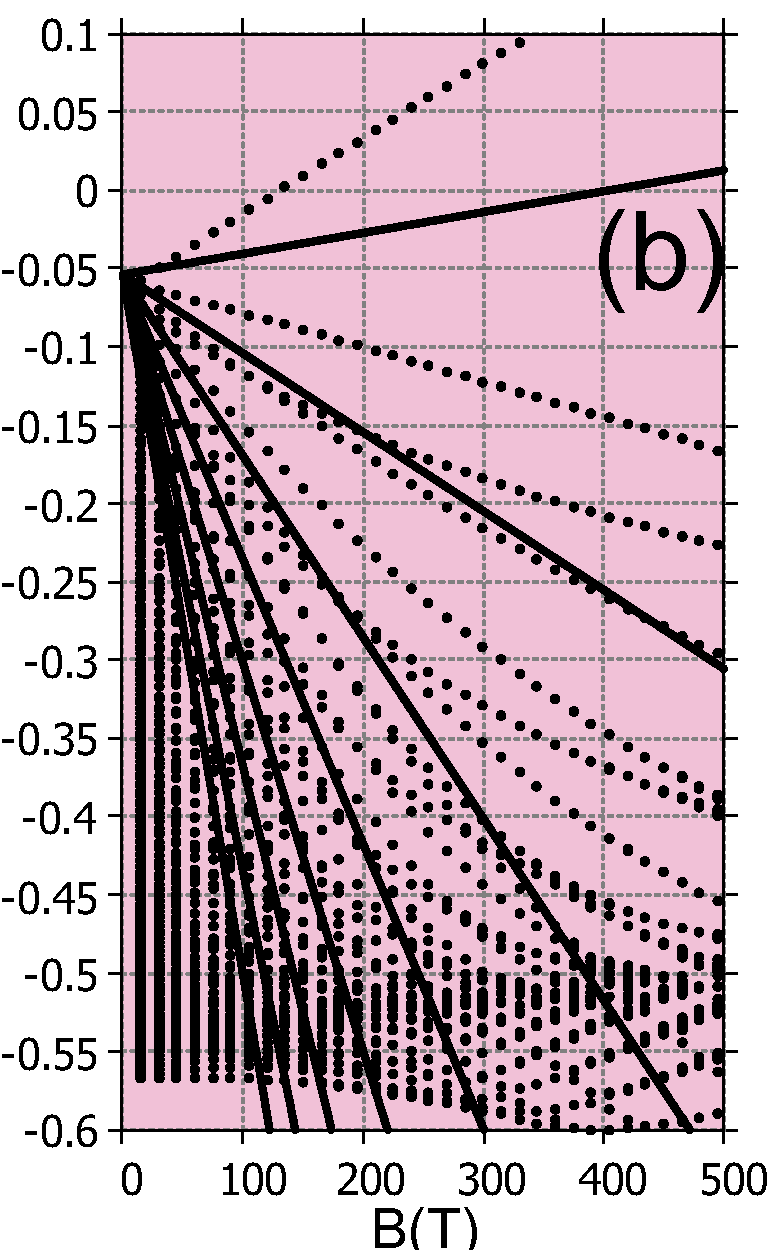
\includegraphics[width=0.85\textwidth,height=1.2\linewidth]{pic/landaulevel_3band_q_797_EF_approx_solution.pdf}}
%	\end{subfigure}
%	\begin{subfigure}[b]{0.49\textwidth}
%		\centering
%		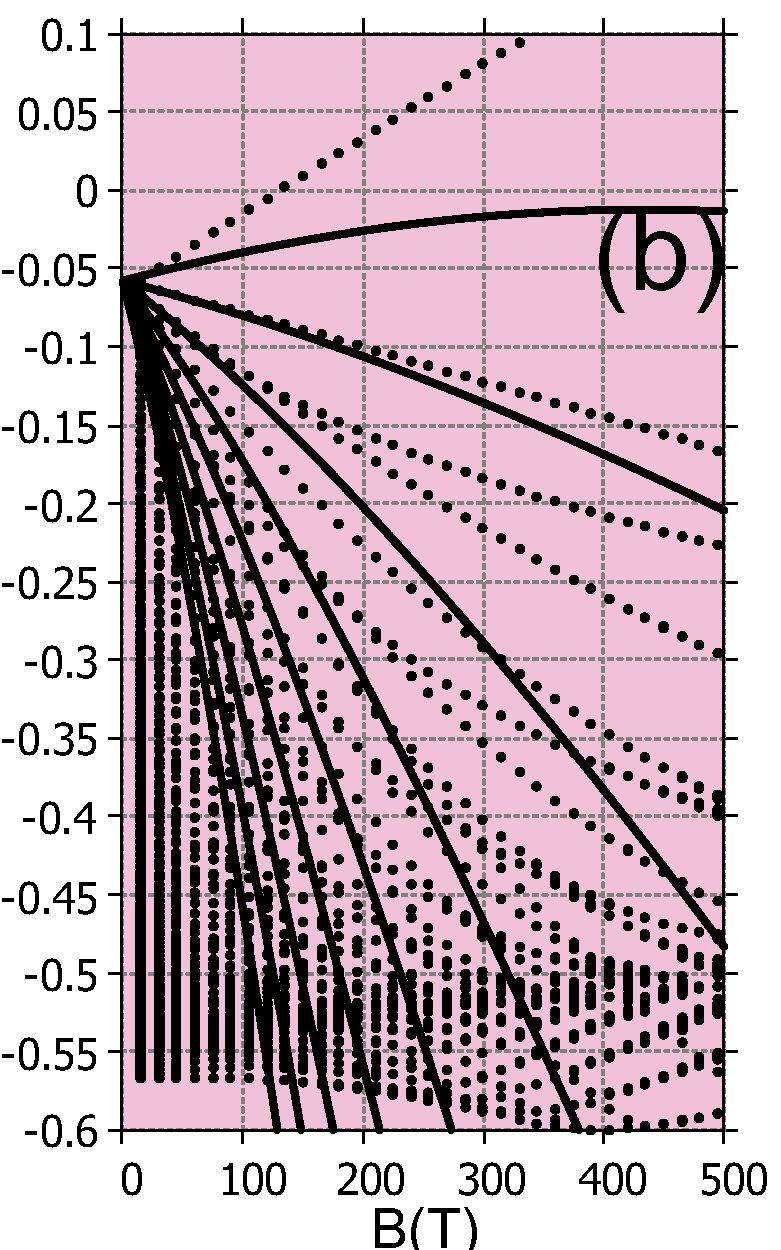
\includegraphics[width=0.85\textwidth,height=1.2\linewidth]{pic/landaulevel_3band_q_797_EF_analytics_solution.pdf}
%	\end{subfigure}
%	\caption{
%		A comparision bewteen two methods, figure on the right take data from maple, both depicts Landau levels.
%	}
%\end{figure*}
%\chapter{Fermi energy}
%Given
%\begin{gather}
%	E_{\lambda} = \frac{\hbar^{2} k^{2}}{2m} + \left(\lambda + \frac{1}{2}\right) \hbar \omega_{c},
%\end{gather}
%and
%\begin{gather}
%	n_{0} = \sum_{\lambda=0}^{\lambda_{\text{max}}} f(E_{F}) = \sum_{\lambda=0}^{\lambda_{\text{max}}} \tfrac{1}{\exp[\frac{E_{\lambda} - E_{F}}{k_{B}T}] + 1},
%\end{gather}
%In this work, we had choose $\lambda_{\text{max}} = 30$, if $\lambda \geq \lambda_{\text{max}}$ then $n_{0} = 0$ due to the property of Fermi level. With the aid of Eq (2.50), we rewrite (D.2) in the form as
%\begin{gather}
%	n_{0} = \sum_{ \lambda = 0}^{\lambda_{\text{max}}} \f{1}{\exp[\tfrac{t_{0} \left(6 - 8\pi\sqrt{3} \frac{p}{q}( \lambda + 1 /2)\right) + \epsilon_{1} - E_{F}}{k_{B} T}] + 1},
%\end{gather}
%with $k_{B}$ is Boltzmann constant, $T= 50$mK, $n_{0} = 2.8\times10^{15}$m$^{-2}$
%\begin{equation}
%	\begin{aligned}
%		E_{F} = - \ln\left[\frac{1-n_{0}}{n_{0}}\right] k_{B}T + E_{n}
%	\end{aligned}
%\end{equation}
%
%Density of states DOS $D(\varepsilon)$ is calculated from
%\begin{gather}
%	\rho(E_{F},T) = \int_{-\infty}^{E_{F}} f\left(\frac{\varepsilon - E_{F}}{k_{B}T}\right) D(\varepsilon) d\varepsilon,
%\end{gather}
%where $f(x) = \frac{1}{e^{x} + 1}$ is the Fermi-Dirac distribution, $T$ is the temperature of the system.

\newpage












%\begin{equation}
%	\begin{aligned}
%		h_{v}
%		\approx & 3(t_{11} + t_{22}) - \f{3a^{2}(t_{11} + t_{22})}{4\hbar^{2}} \f{\hbar e B}{2} ( - a^{\dagger} a^{\dagger} + a^{\dagger}a + a a^{\dagger} - aa ) \\
%		        & - \f{3a^{2}(t_{11} + t_{22})}{4\hbar^{2}} \f{\hbar e B}{2} (aa + a a^{\dagger} + a^{\dagger} a + a^{\dagger} a^{\dagger})                       \\
%		        & - \f{a^{3} t_{12}}{4\hbar^{2}} \f{\hbar e B}{2} ( - a^{\dagger} a^{\dagger} + a^{\dagger}a + a a^{\dagger} - aa ) \Pi_{x}                       \\
%		        & + \f{a^{3} t_{12}}{4\hbar^{2}} \f{3\hbar e B}{2} ( a^{\dagger} a^{\dagger} + a^{\dagger}a + a a^{\dagger} + aa ) \Pi_{x} + \epsilon_{2}         \\
%		\approx & 3(t_{11} + t_{22}) - \f{3a^{2}(t_{11} + t_{22})}{4\hbar^{2}} \f{\hbar e B}{2}
%	\end{aligned}
%\end{equation}

%Tới đây thì không thể tính ra được vì còn số hạng bậc 3 theo kx ky và $i$ có nghĩa là vẫn còn $\Pi_{x}$. \\
%Tần số cyclotron khi sử dụng như section 2( đã loại bỏ số hạng có $a^3$ và $a^4$)
%\begin{gather}
%	w_{c} = \f{eB}{m^{*}} = \f{4 \pi \sqrt{3} (t_{11} + t_{22})}{\hbar} \f{p}{q},
%\end{gather}
%and
%\begin{gather}
%	E \approx (t_{11} + t_{22}) \left(3 - 4\pi \sqrt{3} \f{p}{q}(n + 1/ 2)\right) + \epsilon_{2},
%\end{gather}
%\begin{figure}[H]
%	\centering
%	\includegraphics[width=0.5\linewidth,height=0.5\linewidth]{pic/wrong.png}
%	\caption{\label{}  C.13}
%\end{figure}
%
%
%
%By using Taylor expansion, Hamiltonian Eq()
%\begin{equation}
%	\begin{aligned}
%		h_{0}  & = t_{0} (6 - \frac{3}{2} a^{2} (k_{x}^{2} + k_{y}^{2})) + \epsilon_{1}                                                                         \\
%		h_{1}  & = i t_{1} 3a k_{x} - \frac{3}{2} t_{2} a^{2} k_{x}k_{y}                                                                                        \\
%		h_{2}  & = 2 t_{2} (\frac{3}{8} a^{2} k_{x}^{2} + \frac{3}{8} a^{2} k_{y}^{2}) + i 3 t_{1} a k_{y}                                                      \\
%		h_{11} & = (t_{11} + 3 t_{22}) (1 - \frac{1}{8}a^{2} k_{x}^{2} - \frac{3}{8}a^{2} k_{y}^{2}) + 2 t_{11}(1 - \frac{1}{2} a^{2} k_{x}^{2}) + \epsilon_{2} \\
%		h_{22} & = (3 t_{11} + t_{22}) (1 - \frac{1}{8}a^{2} k_{x}^{2} - \frac{3}{8}a^{2} k_{y}^{2}) + 2 t_{22}(1 - \frac{1}{2} a^{2} k_{x}^{2}) + \epsilon_{2} \\
%		h_{12} & = \sqrt{3} (t_{22} - t_{11}) a^{2} k_{x} k_{y}
%		%+ 4i t_{12} \frac{a k_{x}}{2} ( \frac{3a^{2} k_{y}^{2}}{8} - \frac{a^{2} k_{x}^{2}}{8})
%	\end{aligned}
%\end{equation}
%By using substitution $\hbar \mathbf{k} = \boldsymbol{\Pi} + e \mathbf{A}$
%\begin{equation}
%	\begin{aligned}
%		h_{0}  & = t_{0} (6 - \frac{3}{2\hbar^{2}} a^{2} (\Pi_{x}^{2} + (\Pi_{y} + e Bx)^{2})) + \epsilon_{1}                                                                 \\
%		h_{1}  & = i t_{1} \frac{3}{\hbar}a \Pi_{x} - \frac{3}{2\hbar^{2}} t_{2} a^{2} \Pi_{x}(\Pi_{y} + eBx)                                                                 \\
%		h_{2}  & = 2 t_{2} (\frac{3}{8\hbar^{2}} a^{2} \Pi_{x}^{2} + \frac{3}{8\hbar^{2}} a^{2} (\Pi_{y} + eBx)^{2}) + i \frac{3}{\hbar} t_{1} a (\Pi_{y} + eBx)              \\
%		h_{11} & = (t_{11} + 3 t_{22}) (1 - \frac{1}{8}a^{2} \Pi_{x}^{2} - \frac{3}{8}a^{2} (\Pi_{y} + eBx)^{2}) + 2 t_{11}(1 - \frac{1}{2} a^{2} \Pi_{x}^{2}) + \epsilon_{2} \\
%		h_{22} & = (3 t_{11} + t_{22}) (1 - \frac{1}{8}a^{2} \Pi_{x}^{2} - \frac{3}{8}a^{2} (\Pi_{y} + eBx)^{2}) + 2 t_{22}(1 - \frac{1}{2} a^{2} \Pi_{x}^{2}) + \epsilon_{2} \\
%		h_{12} & = \sqrt{3} (t_{22} - t_{11}) a^{2} \Pi_{x} (\Pi_{y} + eBx)
%		%+ 4i t_{12} \frac{a k_{x}}{2} ( \frac{3a^{2} k_{y}^{2}}{8} - \frac{a^{2} k_{x}^{2}}{8})
%	\end{aligned}
%\end{equation}
%Hamiltonian in term of ladder operators
%\begin{equation}
%	\begin{aligned}
%		h_{0} &= -6t_{0}a^{2}( a^{\dagger} a^{-} + \tfrac{1}{2}) + 6t_{0} + \epsilon_{1} \\
%		h_{1} &= 3 t_{1} a ( a^{-} - a^{\dagger}) - \tfrac{3 i t_{2} a^{2}}{2}(a^{\dagger} a^{\dagger} - a^{-}a^{-} - 1) \\
%		h_{2} &= 3 i t_{1} a (a^{\dagger} + a^{-}) + \tfrac{3t_{2} a^{2}}{2}(a^{\dagger} a^{\dagger} + a^{-} a^{-})\\
%		h_{11} &=	3 (t_{11} + t_{22}) + \tfrac{3t_{11}a^{2}}{4}( a^{\dagger}a^{\dagger} + a^{-} a^{-} ) - 3 (t_{11} + t_{22})a^{2} (a^{\dagger} a^{-} + \tfrac{1}{2}) + \epsilon_{2} \\
%		h_{22} &=	3 (t_{11} + t_{22}) + \tfrac{3t_{22}a^{2}}{4}( a^{\dagger}a^{\dagger} + a^{-} a^{-} ) - 3 (t_{11} + t_{22})a^{2} (a^{\dagger} a^{-} + \tfrac{1}{2}) + \epsilon_{2} \\
%		h_{12} &= \sqrt{3}i (t_{22} - t_{11}) (a^{\dagger} a^{\dagger} - a^{-} a^{-} - 1) 
%	\end{aligned}
%\end{equation}





%\chapter{Phase factor}
%\begin{equation}
%	\begin{aligned}
%		H_{\mu\mu'}^{jj'}(\mathbf{k})
%		& = \sum_{\mathbf{R}} e^{\frac{ie}{\hbar}\int_{0}^{\mathbf{R}}A(\mathbf{r'})d\mathbf{r'}}e^{i\mathbf{k\cdot R}} E_{\mu\mu'}^{jj'}(\mathbf{R})                                                                                                                                                   \\
%		& = E_{\mu\mu'}^{jj'}(\mathbf{0}) + e^{\frac{ie}{\hbar}\int_{0}^{\mathbf{R_1}}\mathbf{A(\mathbf{r'})}\cdot d\mathbf{r'}}e^{i\mathbf{k\cdot R_1}} E_{\mu\mu'}^{jj'}(\mathbf{R_1})                                                                                                                \\
%		& + e^{\frac{ie}{\hbar}\int_{0}^{\mathbf{R_2}}\mathbf{A(\mathbf{r'})}\cdot d\mathbf{r'}}e^{i\mathbf{k\cdot R_2}} E_{\mu\mu'}^{jj'}(\mathbf{R_2}) + e^{\frac{ie}{\hbar}\int_{0}^{\mathbf{R_3}}\mathbf{A(\mathbf{r'})}\cdot d\mathbf{r'}}e^{i\mathbf{k\cdot R_3}} E_{\mu\mu'}^{jj'}(\mathbf{R_3}) \\
%		& + e^{\frac{ie}{\hbar}\int_{0}^{\mathbf{R_4}}\mathbf{A(\mathbf{r'})}\cdot d\mathbf{r'}}e^{i\mathbf{k\cdot R_4}} E_{\mu\mu'}^{jj'}(\mathbf{R_4}) + e^{\frac{ie}{\hbar}\int_{0}^{\mathbf{R_5}}\mathbf{A(\mathbf{r'})}\cdot d\mathbf{r'}}e^{i\mathbf{k\cdot R_5}} E_{\mu\mu'}^{jj'}(\mathbf{R_5}) \\
%		& + e^{\frac{ie}{\hbar}\int_{0}^{\mathbf{R_6}}\mathbf{A(\mathbf{r'})}\cdot d\mathbf{r'}}e^{i\mathbf{k\cdot R_6}} E_{\mu\mu'}^{jj'}(\mathbf{R_6})\\
%		&=  E_{\mu\mu'}^{jj'}(\mathbf{0}) + e^{\frac{ie}{\hbar} Bx \int_{\mathbf{0}}^{\mathbf{R}_{1}}dy} e^{i k_{x} a} E_{\mu\mu'}^{jj'}(\mathbf{R}_{1}) + e^{\frac{ie}{\hbar} Bx \int_{\mathbf{0}}^{\mathbf{R}_{2}}dy} e^{i k_{x}\frac{a}{2}} e^{-i k_{y} \frac{a\sqrt{3}}{2}} E_{\mu\mu'}^{jj'}(\mathbf{R}_{2}) \\
%		&+ e^{\frac{ie}{\hbar} Bx \int_{\mathbf{0}}^{\mathbf{R}_{3}}dy} e^{-i k_{x} \frac{a}{2}} e^{-i k_{y} \frac{a\sqrt{3}}{2}} E_{\mu\mu'}^{jj'}(\mathbf{R}_{3}) + e^{\frac{ie}{\hbar} Bx \int_{\mathbf{0}}^{\mathbf{R}_{4}}dy} e^{-i k_{x} a} E_{\mu\mu'}^{jj'}(\mathbf{R}_{4})\\
%		&+ e^{\frac{ie}{\hbar} Bx \int_{\mathbf{0}}^{\mathbf{R}_{5}}dy} e^{-i k_{x} a} e^{i k_{y} \frac{a\sqrt{3}}{2}} E_{\mu\mu'}^{jj'}(\mathbf{R}_{5}) + e^{\frac{ie}{\hbar} Bx \int_{\mathbf{0}}^{\mathbf{R}_{6}}dy} e^{i k_{x} a} e^{i k_{y} \frac{a\sqrt{3}}{2}} E_{\mu\mu'}^{jj'}(\mathbf{R}_{6})\\
%		&=  E_{\mu\mu'}^{jj'}(\mathbf{0}) + e^{0} e^{i k_{x} a} E_{\mu\mu'}^{jj'}(\mathbf{R}_{1}) + e^{-\frac{ie}{\hbar} B x \frac{a\sqrt{3}}{2}} e^{i k_{x}\frac{a}{2}} e^{-i k_{y} \frac{a\sqrt{3}}{2}} E_{\mu\mu'}^{jj'}(\mathbf{R}_{2}) \\
%		&+ e^{-\frac{ie}{\hbar} B x \frac{a\sqrt{3}}{2}} e^{-i k_{x} \frac{a}{2}} e^{-i k_{y} \frac{a\sqrt{3}}{2}} E_{\mu\mu'}^{jj'}(\mathbf{R}_{3}) + e^{0} e^{-i k_{x} a} E_{\mu\mu'}^{jj'}(\mathbf{R}_{4})\\
%		&+ e^{\frac{ie}{\hbar} B x \frac{a\sqrt{3}}{2}} e^{-i k_{x} a} e^{i k_{y} \frac{a\sqrt{3}}{2}} E_{\mu\mu'}^{jj'}(\mathbf{R}_{5}) + e^{\frac{ie}{\hbar} B x \frac{a\sqrt{3}}{2}} e^{i k_{x} a} e^{i k_{y} \frac{a\sqrt{3}}{2}} E_{\mu\mu'}^{jj'}(\mathbf{R}_{6})
%	\end{aligned}
%\end{equation}
%Applying the BCH formula, and using the commutation relation $\left[x, p_{x}\right] = i \hbar$, we have
%\begin{equation}
%	\begin{aligned}
%		e^{i\left( \frac{\hbar k_{x}}{\hbar} - \frac{e}{\hbar}Bx \sqrt{3}\right) \frac{a}{2}}
%		= e^{i\left( p_{x} - \sqrt{3}eBx\right) \frac{a}{2 \hbar}} = 
%	\end{aligned}
%\end{equation}
%\chapter{Matrix}
%
%\begin{equation}
%	\rotatebox{90}{$
%		\begin{aligned}
%			h_{1}
%			& =
%			\begin{pNiceArray}{c|c|c|c|c|c|c|c}
%				\scriptstyle 0                    & \Block{1-1}{\scriptstyle 2t_{1}\cos\zeta_{1}  \\ \scriptstyle + i \sqrt{3} t_{2} \sin\zeta_{1}}   &\scriptstyle t_{1}               & \scriptstyle 0                   & \cdots & \scriptstyle 0                    & \scriptstyle -t_{1}                & \Block{1-1}{\scriptstyle -2t_{1}\cos\gamma_{1}  \\ \scriptstyle - i \sqrt{3} t_{2} \sin\gamma_{1}} \\
%				\hline
%				\Block{1-1}{\scriptstyle -2t_{1}\cos\gamma_{2}  \\ \scriptstyle - i \sqrt{3} t_{2} \sin\gamma_{2}} & \scriptstyle 0                     & \Block{1-1}{\scriptstyle 2t_{1}\cos\zeta_{2}  \\ \scriptstyle + i \sqrt{3} t_{2} \sin\zeta_{2}} &\scriptstyle t_{1}               & \scriptstyle 0      & \cdots               & \scriptstyle 0                    & \scriptstyle -t_{1}                \\
%				\hline
%				\scriptstyle -t_{1}                & \Block{1-1}{\scriptstyle -2t_{1}\cos\gamma_{3}  \\ \scriptstyle - i \sqrt{3} t_{2} \sin\gamma_{3}} & \scriptstyle 0                   & \Block{1-1}{\scriptstyle 2t_{1}\cos\zeta_{3}  \\ \scriptstyle + i \sqrt{3} t_{2} \sin\zeta_{3}} &\scriptstyle t_{1}  & \scriptstyle 0                    & \cdots                    & \scriptstyle 0                    \\
%				\hline
%				\vdots               & \vdots                & \vdots              & \vdots              & \vdots & \vdots               & \vdots               & \vdots               \\
%				\hline
%				t_{1}                & \scriptstyle 0                     & \cdots              & \scriptstyle 0                   & \scriptstyle -t_{1}  & \Block{1-1}{\scriptstyle -2t_{1}\cos\gamma_{q - 1}  \\ \scriptstyle - i \sqrt{3} t_{2} \sin\gamma_{q - 1}} & \scriptstyle 0                    & \Block{1-1}{\scriptstyle 2t_{1}\cos\zeta_{q - 1}  \\ \scriptstyle + i \sqrt{3} t_{2} \sin\zeta_{q - 1}}  \\
%				\hline
%				\Block{1-1}{\scriptstyle 2t_{1}\cos\zeta_{q}  \\ \scriptstyle + i \sqrt{3} t_{2} \sin\zeta_{q}}  &\scriptstyle t_{1}                 & \cdots              & \scriptstyle 0                   & \scriptstyle 0      & \scriptstyle -t_{1}                & \Block{1-1}{\scriptstyle -2t_{1}\cos\gamma_{q}  \\ \scriptstyle - i \sqrt{3} t_{2} \sin\gamma_{q}} & \scriptstyle 0                    \\
%			\end{pNiceArray}
%		\end{aligned}$}
%\end{equation}


\nocite{*}
\renewcommand{\bibname}{REFERENCES}
\bibliographystyle{unsrt}
\bibliography{refs}








































































































































































































































































































































































































































































































































































































































































\end{document}
